\chapter{Additional Topics}
\section{The de Rham cohomology groups}
\subsection{The de Rham cohomology groups}
We studied the closed $1$-form
\[\omega=\frac{xdy-ydx}{x^2+y^2},\]
and showed that it is not exact on $\R^2-\{0\}$, but it is exact on some smaller domains such as the right half-plane $H=\{(x,y):x>0\}$, where it is equal to $d\theta$.\par
As we will see later, this behavior is typical: closed forms are always \textbf{locally exact}, so whether a given closed form is exact depends on the global shape of the domain. To capture this dependence, we make the following definitions.\par
Let $M$ be a smooth manifold with or without boundary, and let $p$ be a nonnegative integer. Because $d:\Omega^p(M)\to\Omega^{p+1}(M)$ is linear, its kernel and image are
linear subspaces. We define
\[\begin{array}{l}Z^p(M)=\ker d=\{\text{closed $p$-form on $M$}\},\\
B^p(M)=\im d=\{\text{exact $p$-form on $M$}\}.
\end{array}\]
By convention, we consider $\Omega^p(M)$ to be the zero vector space when $p<0$ or $p>n=\dim M$, so that, for example, $B^0(M)=0$ and $Z^n=\Omega^n(M)$.\par
The fact that every exact form is closed implies that $B^p(M)\sub Z^p(M)$. Thus, it makes sense to define the \textbf{de Rham cohomology group} in degree $p$ of $M$ to be the quotient vector space
\[H^p_{dR}(M)=\frac{Z^p(M)}{B^p(M)}.\]
It is clear that $H^p_{dR}(M)=0$ for $p<0$ or $p>\dim M$, because $Z^p(M)=0$ in those cases. For $0\leq p\leq n$, the definition implies that $H^p_{dR}(M)=0$ if and only if every closed $p$-form on $M$ is exact.
\begin{example}
The fact that there is a closed $1$-form on $\R^2-\{0\}$ that is not exact means that $H^1_{dR}(\R^2-\{0\})\neq 0$. On the other hand, the Poincar\'e lemma for $1$-forms 
implies that $H^1_{dR}(U)=0$ for any star-shaped open subset $U\sub\R^n$.
\end{example}
The first order of business is to show that the de Rham groups are diffeomorphism invariants. For any closed $p$-form $\omega$ on $M$, we let $[\omega]$ denote the equivalence class of $\omega$ in $H^p_{dR}(M)$, called the \textbf{cohomology class} of $\omega$. If $[\omega]=[\omega']$, we say that $\omega$ and $\omega'$ are \textbf{cohomologous}.
\begin{proposition}[\textbf{Induced Cohomology Maps}]\label{cohomology induced map}
For any smooth map $F:M\to N$ between smooth manifolds with or without boundary, the pullback $F^*:\Omega^p(N)\to\Omega^p(M)$ carries $Z^p(N)$ into $Z^p(M)$ and $B^p(N)$ into $B^p(M)$. It thus descends to a linear map, still denoted by $F^*$, from $H^p_{dR}(N)$ to $H^p_{dR}(M)$, called the \textbf{induced cohomology map}. It has the following properties:
\begin{itemize}
\item[(a)] If $G:N\to P$ is another smooth map, then $(G\circ F)^*=F^*\circ G^*$.
\item[(b)] If $\mathrm{id}$ denotes the identity map of $M$, then $\mathrm{id}^*$ is the identity map of $H^p_{dR}(M)$.
\end{itemize}
\end{proposition}
\begin{proof}
If $\omega$ is closed, then $d(F^*\omega)=f^*d\omega=0$, so $F^*\omega$ is also closed. If $\omega=d\eta$ is exact, then $F^*\omega=F^*(d\eta)=d(F^*\eta)$, which is also exact. Therefore, $F^*$ maps $Z^p(N)$ into $Z^p(M)$ and $B^p(N)$ into $B^p(M)$. The induced cohomology map is defined in the obvious way: for a closed $p$-form $\omega$, let
\[F^*[\omega]=[F^*\omega].\]
The rest is immediate.
\end{proof}
The next two corollaries are immediate.
\begin{corollary}[\textbf{Functoriality}]
For any integer $p$, the assignment $M\mapsto H^p_{dR}(M),F\mapsto F^*$ is a contravariant functor from the category of smooth manifolds with boundary to the category of real vector spaces.
\end{corollary}
\begin{corollary}[\textbf{Diffeomorphism Invariance of de Rham Cohomology}]
Diffeomorphic smooth manifolds $($with or without boundary$)$ have isomorphic de Rham cohomology groups.
\end{corollary}
\paragraph{Elementary computations}
The direct computation of the de Rham groups is not easy in general. However, there are a number of special cases that can be easily computed by various techniques. 
\begin{proposition}[\textbf{Cohomology of Disjoint Unions}]
Let $\{M_j\}$ be a countable collection of smooth $n$-manifolds with or without boundary, and let $M=\amalg_jM_j$. For each $p$, the inclusion maps $\iota_j:M_j\hookrightarrow M$ induce an isomorphism from $H^p_{dR}(M)$ to the direct product space $\prod_jH^p_{dR}(M_j)$.
\end{proposition}
Because of this proposition, each de Rham group of a disconnected manifold is just the direct product of the corresponding groups of its components. Thus, we can concentrate henceforth on computing the de Rham groups of connected manifolds. Next we give an explicit characterization of de Rham cohomology in degree zero.
\begin{proposition}[\textbf{Cohomology in Degree Zero}]\label{cohomology degree 0}
If $M$ is a connected smooth manifold with or without boundary, then $H^0_{dR}(M)$ is equal to the space of constant functions and is therefore $1$-dimensional.
\end{proposition}
\begin{proof}
Because there are no $(-1)$-forms, $B^0(M)=0$. A closed $0$-form is a smooth real-valued function $f$ such that $df=0$, and since $M$ is connected, this is true if
and only if $f$ is constant. Therefore $H^0_{dR}(M)=Z^0(M)=\{\text{constant}\}$.
\end{proof}
\begin{corollary}[\textbf{Cohomology of Zero-Manifolds}]
Suppose $M$ is a manifold of dimension $0$. Then $H^0_{dR}(M)$ is a direct product of $1$-dimensional vector spaces, one for each point of $M$, and all other de Rham cohomology groups of $M$ are zero.
\end{corollary}
\subsection{Homotopy invariance}
The underlying fact that allows us to prove the homotopy invariance of de Rham cohomology is that homotopic smooth maps induce the same cohomology map. To motivate the proof, suppose $F,G:M\to N$ are smooth maps, and let us think about what it means to prove that $F^*=G^*$. Given a closed $p$-form $\omega$ on $N$, we need somehow to produce a $(p-1)$-form $\eta$ on $M$ such that
\[G^*\omega-F^*\omega=d\eta.\]
from which it follows that $[G^*\omega]-[F^*\omega]=0$. One might hope to construct $\eta$ in a systematic way, resulting in a map $h$ from closed $p$-forms on $N$ to $(p-1)$-forms on $M$ that satisfies 
\[d(h\omega)=G^*\omega-F^*\omega.\]
Instead of defining $h\omega$ only when $\omega$ is closed, it turns out to be far simpler to define a map $h$ from the space of all smooth $p$-forms on $N$ to the space of smooth $(p-1)$-forms on $M$. Such a map cannot satisfy our desired formula, but instead we will find a family of such maps, one for each $p$, satisfying
\begin{align}\label{cochain homotopy def}
d(h\omega)+h(d\omega)=G^*\omega-F^*\omega.
\end{align}
In general, if $F,G:M\to N$ are smooth maps, a collection of linear maps $h:\Omega^p(N)\to\Omega^{p-1}(M)$ such that $(\ref{cochain homotopy def})$ is satisfied for all $\omega$ is called a homotopy operator between $F^*$ and $G^*$. (The term cochain homotopy is used frequently in the algebraic topology literature.) The next proposition follows immediately from the argument in the preceding paragraph.
\begin{proposition}
Suppose $M$ and $N$ are smooth manifolds with or without boundary. If $F:M\to N$ are smooth maps and there exists a homotopy operator between the pullback maps $F^*$ and $G^*$, then the induced cohomology maps $F^*$ and $G^*$ are equal.
\end{proposition}
The key to our proof of homotopy invariance is to construct a homotopy operator
first in the following special case. Let $M$ be a smooth manifold with or without boundary, and for each $t\in I$, let it $i_t:M\to M\times I$ be the map
\[i_t(x)=(x,t).\]
If $M$ has empty boundary, then $M\times I$ is a smooth manifold with boundary, and all of the results above apply to it. But if $\partial M\neq\emp$, then $M\times I$ has to be considered as a smooth manifold with corners. It is straightforward to check that the definitions of the de Rham groups and induced homomorphisms make perfectly good sense on manifolds with corners, and \cref{cohomology induced map} is valid in that context as well.
\begin{lemma}[\textbf{Existence of a Homotopy Operator}]
For any smooth manifold $M$ with or without boundary, there exists a homotopy operator between the two maps $i_0^*,i_1^*:\Omega^*(M\times I)\to\Omega^*(M)$.
\end{lemma}
\begin{proof}
For each $p$, we need to define a linear map $h:\Omega^p(M)\to\Omega^{p-1}(M)$ such that
\begin{align}\label{cochain homotopy-1}
h(d\omega)+d(h\omega)=i_1^*\omega-i_0^*\omega.
\end{align}
Let $s$ denote the standard coordinate on $\R$, and let $S$ be the vector field on $M\times\R$ given by $S_{(q,s)}=(0,\partial/\partial s|_s)$ under the usual identification $T_{(q,s)}(M\times\R)\approx T_qM\oplus T_s\R$. Given a smooth $p$-form $\omega$ on $M\times I$, define
\[h\omega=\int_{0}^{1}i_t^*(S\intprod\omega)dt.\]
More specifically, for any $q\in M$, this means
\[(h\omega)_q=\int_{0}^{1}i_t^*\big((S\intprod\omega)_{(q,t)}\big)dt.\]
where the integrand is interpreted as a function of $t$ with values in the vector space $\bigwedge^{p-1}(T^*_qM)$. We can compute $d(h\omega)$ at any point by differentiating under the integral sign in local coordinates, which yields
\[d(h\omega)=\int_{0}^{1}d\big(i_t^*(S\intprod\omega)\big)dt.\]
Therefore, using Cartan's magic formula, we obtain
\begin{align*}
d(h\omega)+h(d\omega)&=\int_{0}^{1}d\big(i_t^*(S\intprod\omega)\big)dt+\int_{0}^{1}i_t^*(S\intprod d\omega)dt\\
&=\int_{0}^{1}i_t^*\big(d(S\intprod\omega)+S\intprod d\omega\big)dt\\
&=\int_{0}^{1}i_t^*(\mathfrak{L}_S\omega)dt.
\end{align*}
To simplify this last expression, we use the flow of $S$ on $M\times\R$. (If $M$ has
nonempty boundary, note that $S$ is tangent to $\partial(M\times\R)=\partial M\times\R$.) The flow is given explicitly by $\theta_t(q,s)=(q,t+s)$, so $S$ is complete. 
It follows that we can write it $i_t=\theta_t\circ i_0$, and therefore by \cref{Lie der tensor t_0},
\[i_t^*(\mathfrak{L}_S\omega)=i_0^*\circ\theta_t^*(\mathfrak{L}_S\omega)=i_0^*\Big(\frac{d}{dt}(\theta_t^*\omega)\Big)=\frac{d}{dt}i_0^*(\theta_t^*\omega)=\frac{d}{dt}i_t^*\omega.\]
Applying the fundamental theorem of calculus, we obtain $(\ref{cochain homotopy-1})$.
\end{proof}
\begin{proposition}\label{cohomology homotopy map}
Suppose $M$ and $N$ are smooth manifolds with or without boundary, and $F,G:M\to N$ are homotopic smooth maps. For every $p$, the induced cohomology maps $F^*$ and $G^*$ are equal.
\end{proposition}
\begin{proof}
The preceding lemma implies that the two cohomology maps $i_0^*$ and $i_1^*$ are equal. By \cref{homotopy smooth boundary}, there is a smooth homotopy $H:M\times I\to N$ from $F$ to $G$. Because $F=H\circ i_0$ and $G=H\circ i_1$, \cref{cohomology induced map} implies
\[F^*=i_0^*\circ H^*=i_1^*\circ H=G^*.\]
\end{proof}
\begin{theorem}[\textbf{Homotopy Invariance of de Rham Cohomology}]
If $M$ and $N$ are homotopy equivalent smooth manifolds with or without boundary, then $H^p_{dR}(M)\cong H^p_{dR}(N)$ for each $p$. The isomorphisms are induced by any smooth homotopy equivalence $F:M\to N$.
\end{theorem}
\begin{proof}
Suppose $F:M\to N$ is a homotopy equivalence, with homotopy inverse $G:N\to M$. By the Whitney approximation theorem, there are smooth maps $\widetilde{F}:M\to N$ homotopic to $F$ and $\widetilde{G}:N\to M$ homotopic to $G$. Because homotopy is preserved by composition, it follows that 
\[\widetilde{F}\circ\widetilde{G}\simeq F\circ G\simeq\mathrm{id}_M,\quad \widetilde{G}\circ\widetilde{F}\simeq G\circ F\simeq\mathrm{id}_N.\]
so $\widetilde{F}$ and $\widetilde{G}$ are homotopy inverses of each other.\par
\cref{cohomology homotopy map} shows that, on cohomology,
\[\widetilde{F}^*\circ\widetilde{G}^*=\mathrm{id},\quad \widetilde{G}^*\circ\widetilde{F}^*=\mathrm{id}.\]
so $\widetilde{F}^*:H^p_{dR}(M)\to H^p_{dR}(N)$ is an isomorphism.
\end{proof}
Because every homeomorphism is a homotopy equivalence, the next corollary is immediate.
\begin{corollary}[\textbf{Topological Invariance of de Rham Cohomology}]
The de Rham cohomology groups are topological invariants: if $M$ and $N$ are homeomorphic smooth manifolds with or without boundary, then their de Rham cohomology
groups are isomorphic.
\end{corollary}
This result is remarkable, because the definition of the de Rham groups of M
is intimately tied up with its smooth structure, and we had no reason to expect that
different differentiable structures on the same topological manifold should give rise
to the same de Rham groups.
\paragraph{Computations using homotopy invariance}
We can use homotopy invariance to compute a number of de Rham groups. We begin with the simplest case of homotopy equivalence. A topological space $X$ is said to
be \textbf{contractible} if the identity map of $X$ is homotopic to a constant map.
\begin{theorem}[\textbf{Cohomology of Contractible Manifolds}]
If $M$ is a contractible smooth manifold with or without boundary, then $H^p_{dR}(M)=0$ for $p\geq 1$.
\end{theorem}
\begin{theorem}[\textbf{The Poincar\'e Lemma}]
If $U$ is a star-shaped open subset of $\R^n$ or $\H^n$, then $\H^p_{dR}(U)=0$ for $p\geq1$.
\end{theorem}
\begin{proof}
If $U$ is star-shaped with respect to $c$, then it is contractible by the straight-line homotopy $H(x,t)=c+t(x-c)$.
\end{proof}
\begin{corollary}[\textbf{Local Exactness of Closed Forms}]
Let $M$ be a smooth manifold with or without boundary. Each point of $M$ has a neighborhood on which every closed $p$-form is exact for $p\geq 1$.
\end{corollary}
\begin{corollary}[\textbf{Cohomology of Euclidean Spaces and Half-Spaces}]
For any integers $n\geq 0$ and $p\geq1$, we have $H^p_{dR}(\R^n)=H^p_{dR}(\H^n)=0$.
\end{corollary}
Another case in which we can say quite a lot about de Rham cohomology is in degree $1$. Suppose $M$ is a connected smooth manifold and $q$ is any point in $M$. Let $\Hom(\pi_1(M,q),\R)$ denote the set of group homomorphisms from $\pi_1(M,q)$ to the additive group $\R$; it is a vector space under pointwise addition of homomorphisms and multiplication by constants. We define a linear map $\varPhi:H^1_{dR}(M)\to\Hom(\pi_1(M,q),\R)$ as follows: given a cohomology class $[\omega]\in H^1_{dR}(M)$, define $\varPhi[\omega]:\pi_1(M,q)\to\R$ by
\[\varPhi[\omega][\gamma]=\int_{\widetilde{\gamma}}\omega.\]
where $[\gamma]$ is any path homotopy class in $\pi_1(M,q)$, and $\widetilde{\gamma}$ is any piecewise smooth curve representing the same path class.
\begin{theorem}[\textbf{First Cohomology and the Fundamental Group}]\label{cohomology fundamental group}
Suppose $M$ is a connected smooth manifold. For each $q\in M$, the linear map $\varPhi:H^1_{dR}(M)\to\Hom(\pi_1(M,q),\R)$ is an isomorphism.
\end{theorem}
\begin{proof}
Given $[\gamma]\in\pi_1(M,q)$, it follows from the Whitney approximation theorem that there is some smooth closed curve segment $\widetilde{\gamma}$ in the same path class as $\gamma$, and from \cref{int homotopy path} that $\int_{\widetilde{\gamma}}\omega$ gives the same result for every piecewise smooth curve $\widetilde{\gamma}$ in the given class. Moreover, if $\widetilde{\omega}$ is another smooth $1$-form in the same cohomology class as $\omega$, then $\omega-\widetilde{\omega}=df$ for some smooth function $f$, which implies
\[\int_{\widetilde{\gamma}}\omega-\int_{\widetilde{\gamma}}\widetilde{\omega}=\int_{\widetilde{\gamma}}df=f(q)-f(q)=0.\]
Thus $\varPhi$ is well defined. It follows from \cref{line integral prop}(c) that $\varPhi[\omega]$ is a group homomorphism from $\pi_1(M,q)$ to $\R$, and 
from linearity of the line integral that $\varPhi$ itself is a linear map.\par
To see that $\varPhi$ is an isomorphism, we will use the following facts:
\[H_1(M;\R)\cong\mathrm{Ab}(\pi_1(M),q),\quad H^1_{dR}(M)\cong H.\]
The first is the Hurwitz isomorphism, and the second is the de Rham theorem. Now from the observation
\[\Hom(\pi_1(M,q),\R)=\Hom(\mathrm{Ab}(\pi_1(M,q)),\R)\]
and that $\varPhi$ is exactly the isomorphism in the de Rham theorem, the claim follows.
\end{proof}
It follows from \cref{simply con 1 form} that $H^1_{dR}(M)=0$ when $M$ is simply connected. The next corollary generalizes that result.
\begin{proposition}
A group $G$ is called a \textbf{torsion group} if for each $g\in G$ there exists an integer $k$ such that $g^k=1$. If $M$ is a connected smooth manifold whose fundamental group is a torsion group, then $H^1_{dR}(M)=0$.
\end{proposition}
\begin{proof}
There are no nontrivial homomorphisms from a torsion group to $\R$.
\end{proof}
\begin{corollary}\label{cohomology fundamental finite}
If $M$ is connected with finite fundamental group, then $H^1_{dR}(M)=0$.
\end{corollary}
\begin{proof}
Any finite group is torsion.
\end{proof}
\subsection{The Mayer-Vietoris theorem}
Suppose $M$ is a smooth manifold with or without boundary, and $U,V$ are open subsets ofM such that $M=U\cup V$. We have four inclusions,
\[\begin{tikzcd}[row sep=12pt,column sep=12pt]
&U\ar[rd,"j_U"]&\\
U\cap V\ar[ru,"i_U"]\ar[rd,swap,"i_V"]&&M\\
&V\ar[ru,swap,"j_V"]&
\end{tikzcd}\]
which induce pullback maps on differential forms,
\[\begin{tikzcd}[row sep=12pt,column sep=12pt]
&\Omega^p(U)\ar[rd,"i_U^*"]&\\
\Omega^p(M)\ar[ru,"j_U^*"]\ar[rd,swap,"j_V^*"]&&\Omega^p(U\cap V)\\
&\Omega^p(V)\ar[ru,swap,"i_V^*"]&
\end{tikzcd}\]
as well as corresponding induced cohomology maps. Note that these pullback maps are really just restrictions: for example, $j_U^*\omega=\omega|_U$. Consider the 
following sequence of maps:
\begin{equation}\label{Mayer-1}
\begin{tikzcd}
0\ar[r]&\Omega^p(M)\ar[r,"j_U^*\oplus j_V^*"]&\Omega^p(U)\oplus\Omega^p(V)\ar[r,"i_U^*-i_V^*"]&\Omega^p(U\cap V)\ar[r]&0
\end{tikzcd}
\end{equation}
Because pullbacks commute with $d$, these maps descend to linear maps on the corresponding de Rham cohomology groups.
\begin{theorem}[\textbf{Mayer-Vietoris}]
Let $M$ be a smooth manifold with or without boundary, and let $U,V$ be open subsets of $M$ whose union is $M$. For each $p$, there is a linear map 
$\delta:H^p_{dR}(U\cap V)\to H^{p+1}_{dR}(M)$ such that the following sequence, called the \textbf{Mayer-Vietoris sequence} for the open cover $\{U,V\}$, is exact:
\[\begin{tikzcd}[column sep=small]
\cdots\ar[r]&H^p_{dR}(M)\ar[r,"j_U^*\oplus j_V^*"]&H^p_{dR}(U)\oplus H^p_{dR}(V)\ar[r,"i_U^*-i_V^*"]&H^p_{dR}(U\cap V)\ar[r,"\delta"]&H^{p+1}_{dR}(M)\ar[r]&\cdots
\end{tikzcd}\]
\end{theorem}
\begin{proof}
Suppose $M$ is a smooth manifold with or without boundary, and $U,V$ are open subsets of $M$ whose union is $M$. The heart of the proof is to show that the sequence 
$(\ref{Mayer-1})$ is exact for each $p$. Because pullback maps commute with the exterior derivative, $(\ref{Mayer-1})$ therefore defines a short exact sequence of 
cochain maps, and the Mayer-Vietoris theorem follows immediately from the zigzag lemma.\par
We begin by proving exactness at $\Omega^p(M)$, which just means showing that $j_U^*\oplus j_V^*$ is injective. Suppose that $\sigma\in\Omega^p(M)$ satisfies 
$(j_U^*\oplus j_V^*)\sigma=(\sigma|_U,\sigma|_V)=(0,0)$. This means that the restrictions of $\sigma$ to $U$ and $V$ are both zero. Since $\{U,V\}$ is an open cover of 
$M$, this implies that $\sigma$ is zero.\par
To prove exactness at $\Omega^p(U)\oplus\Omega^p(V)$, first observe that
\[(i_U^*-i_V^*)\circ(j_U^*\oplus j_V^*)=0,\]
which shows that $\im(j_U^*\oplus j_V^*)\sub\ker(i_U^*-i_V^*)$. Conversely, suppose we are given $(\eta,\eta')\in\Omega^p(U)\oplus\Omega^p(V)$ such that 
$i^*(\eta)-j^*(\eta')=0$. This means that $\eta|_{U\cap V}=\eta'|_{U\cap V}$, so there is a global smooth $p$-form $\sigma$ on $M$ defined by
\[\sigma=\begin{cases}
\eta&\text{on }U,\\
\eta'&\text{on }V.
\end{cases}\]
so $\ker(i_U^*-i_V^*)\sub\im(j_U^*\oplus j_V^*)$.\par
Exactness at $\Omega^*(U\cap V)$ means that $i_U^*-i_V^*$ is surjective. This is the only nontrivial part of the proof, and the only part that really uses any properties of smooth manifolds and differential forms.\par
Let $\omega\in\Omega^p(U\cap V)$ be arbitrary. We need to show that there exist $\eta\in\Omega^p(U)$ and $\eta'\in\Omega^p(V)$ such that 
\[\omega=(i_U^*-i_V^*)(\eta,\eta')=i_U^*\eta-i_V^*\eta'=\eta|_{U\cap V}-\eta'_{U\cap V}.\]
Let $\{\rho_U,\rho_V\}$ be a smooth partition of unity subordinate to the open cover $\{U,V\}$ of $M$, and define $\eta\in\Omega^p(U)$ by
\[\eta=\begin{cases}
\rho_V\omega&\text{ on }U\cap V,\\
0&\text{ on }U\setminus\supp(\rho_V).
\end{cases}\]
On the set $(U\cap V)\setminus\supp(\rho_V)$ where these definitions overlap, they both give zero, so this defines $\eta$ as a smooth $p$-form on $U$. Similarly, define $\eta'\in\Omega^p(V)$ by
\[\eta'=\begin{cases}
-\rho_U\omega&\text{ on }U\cap V,\\
0&\text{ on }U\setminus\supp(\rho_U).
\end{cases}\]
Then we have
\[\eta|_{U\cap V}-\eta'|_{U\cap V}=\rho_V\omega+\rho_U\omega=\omega.\]
which was to be proved.
\end{proof}
\begin{corollary}\label{Mayer-Vietoris de Rham connect}
The connecting homomorphism $\delta:H^p_{dR}(U\cap V)\to H^{p+1}_{dR}(M)$ in the Mayer-Vietoris sequence is defined as follows. For each $\omega\in Z^p(U\cap V)$, there 
are $p$-forms $\eta\in\Omega^p(U)$ and $\eta'\in\Omega^p(V)$ such that $\omega=\eta|_{U\cap V}-\eta'|_{U\cap V}$; and then $\delta[\omega]=[\sigma]$, where 
\[\sigma=\begin{cases}
d\eta&\text{ on }U,\\
d\eta'&\text{ on }V.
\end{cases}\]
If $\{\rho_U,\rho_V\}$ is a smooth partition of unity subordinate to $\{U,V\}$, we can take $\eta=\rho_V\omega$ and $\eta'=-\rho_U\omega$, both extended by zero outside 
the supports of $\rho_U$ and $\rho_V$.
\end{corollary}
\begin{proof}
The characterization of the connecting homomorphism is given by the following diagram:
\[\begin{tikzcd}
\ar[r,no head,dotted]&\sigma\ar[r]&(j_U^*\sigma,j_V^*\sigma)\ar[r,no head,dotted]&\ar[r,no head,dotted]&{}\\
\ar[r,no head,dotted]&\ar[r,no head,dotted]\ar[u,no head,dotted]&(\eta,\eta')\ar[r,"i_U^*-i_V^*"]\ar[u,"d"]&\omega\ar[r,no head,dotted]\ar[u,no head,dotted]&{}
\end{tikzcd}\]
We find that $\delta[\omega]=\sigma$, provided there exists $(\eta,\eta')\in\Omega^p(U)\oplus\Omega^p(V)$ such that
\[i_U^*\eta-i_V^*\eta'=\omega,\quad (j_U^*\sigma,j_V^*\sigma)=(d\eta,d\eta').\]
It can be easily checked that our definition of $\sigma$ satisfies the conditions.
\end{proof}
\paragraph{Computations using the Mayer-Vietoris sequence}
Using the Mayer-Vietoris theorem, it is a simple matter to compute all of the de Rham cohomology groups of spheres.
\begin{theorem}[\textbf{Cohomology of Spheres}]\label{cohomology S^n}
For $n\geq1$, the de Rham cohomology groups of $S^n$ are
\[H^p_{dR}(S^n)=\begin{cases}
\R&\text{$p=0$ or $p=n$},\\
0&\text{otherwise}.
\end{cases}\]
The cohomology class of any smooth orientation form is a basis for $H^n_{dR}(S^n)$.
\end{theorem}
\begin{proof}
\cref{cohomology degree 0} shows that $H^0_{dR}(S^n)=\R$, so we need only prove for $p\geq1$. We do so by induction on $n$. For $n=1$, note first that any orientation form on $S^1$ has nonzero integral, so it is not exact by \cref{int exact form} thus $\dim H^1_{dR}(S^1)\geq 1$. On the other hand, \cref{cohomology fundamental group} implies that there is an injective linear map from $H^1_{dR}(S^1)$ into $\Hom(\pi_1(S^1,1),\R)$, which is $1$-dimensional. Thus, $H^1_{dR}(S^1)$ has dimension exactly $1$, and is spanned by the cohomology class of any orientation form.\par
Next, suppose $n\geq 2$ and assume by induction that the theorem is true for $S^{n-1}$. Because $S^n$ is simply connected, $H^1_{dR}(S^n)=0$ by \cref{simply con 1 form}. For $p>1$, we use the Mayer-Vietoris theorem as follows. Let $N$ and $S$ be the north and south poles in $S^n$, respectively, and let $U=S^n-\{S\},V=S^n-\{V\}$. By stereographic projection, both $U$ and $V$ are diffeomorphic to $\R^n$, and thus $U\cap V$ is diffeomorphic to $\R^n-\{0\}$.\par
Part of the Mayer-Vietoris sequence for $\{U,V\}$ read
\[\begin{tikzcd}
H^{p-1}_{dR}(U)\oplus H^{p-1}_{dR}(V)\ar[r]&H^{p-1}_{dR}(U\cap V)\ar[r]&H^{p}_{dR}(S^n)\ar[r]&H^p_{dR}(U)\oplus H^p_{dR}(V)
\end{tikzcd}\]
Because $U$ and $V$ are diffeomorphic to $\R^n$, the groups on both ends are trivial
when $p>1$, which implies that $H^{p-1}_{dR}(U\cap V)\cong H^p_{dR}(S^n)$. Moreover, $U\cap V$ is diffeomorphic to $\R^n-\{0\}$ and therefore homotopy equivalent to $S^{n-1}$, so in the end we conclude that $H^p_{dR}(S^n)\cong H^{p-1}_{dR}(S^{n-1})$ for $p>1$. As in the $n=1$ case, any smooth orientation form on $S^n$ determines a nonzero cohomology class, which therefore spans $H^n_{dR}(S^n)$.
\end{proof}
\begin{corollary}\label{closed n-form S^n exact iff}
Let $\omega$ be a closed $n$-form on $S^n$, then $\omega$ is exact if and only if $\int_{S^n}\omega=0$.
\end{corollary}
\begin{proof}
Let $\omega_{S^n}$ be an orientation form of $S^n$, then by \cref{cohomology S^n} $\omega=a\omega_{S^n}+d\eta$ for some $a\in\R$ and $\eta\in\Omega^{n-1}(S^n)$. Since $\int_{S^n}d\eta=0$, we get the claim.
\end{proof}
\begin{corollary}[\textbf{Cohomology of Punctured Euclidean Space}]\label{cohomology punctured R^n}
Suppose $n\geq2$ and $x\in\R^n$, and let $M=\R^n-\{x\}$. The only nontrivial de Rham groups of $M$ are $H^0_{dR}(M)$ and $H^{n-1}_{dR}(M)$, both of which are $1$-dimensional. A closed $(n-1)$-form $\omega$ on $M$ is exact if and only if $\int_S\omega=0$ for some $($and hence every$)$ $(n-1)$-dimensional sphere $S\sub M$ centered at $x$.\par 
The same statement remains true if $\R^n-\{x\}$ is replaced by $\R^n-\widebar{B}$ for some closed ball $\widebar{B}\sub\R^n$.
\end{corollary}
\begin{proof}
Let $S\sub M$ be any $(n-1)$-dimensional sphere centered at $x$. Because inclusion $\iota:S\hookrightarrow M$ is a homotopy equivalence, $H^p_{dR}(M)\to H^p_{dR}(S)$ is an isomorphism for each $p$, so the assertion about the dimension of $H^p_{dR}(M)$ follows from \cref{cohomology S^n}. If $\omega$ is a closed $(n-1)$-form on $M$, it follows that $\omega$ is exact if and only if $\iota^*\omega$ is exact on $S$, which in turn is true if and only $\int_S\iota^*\omega=0$ by \cref{closed n-form S^n exact iff}.
\end{proof}
\begin{corollary}\label{cohomology U-x}
Suppose $n\geq 2$, $U\sub\R^n$ is any open subset, and $x\in U$. Then $H^{n-1}_{dR}(U-\{x\})\neq 0$.
\end{corollary}
\begin{proof}
Because $U$ is open, there is an $(n-1)$-dimensional sphere $S$ centered at $x$ such that $S\sub U-\{x\}$. Let $\iota:S\hookrightarrow U-\{x\}$ be inclusion and $r:U-\{x\}\to S$ be the radial projection onto $S$. Then $r$ and $\iota$ are smooth with $r\circ\iota=\mathrm{id}_S$. This implies $\iota^*\circ r^*=\mathrm{id}$, and therefore $r^*:H^{n-1}_{dR}(U-\{x\})\to H^{n-1}_{dR}(S)$ is injective. Since $H^{n-1}_{dR}(S)\neq 0$ by \cref{cohomology S^n}, the result follows.
\end{proof}
Here is an important application of the topological invariance of the de Rham cohomology groups. Recall the theorem on invariance of dimension; it is a surprising fact that this purely topological theorem can be proved using de Rham cohomology. Before proving the theorem, we restate it here for convenience.
\begin{proposition}[\textbf{Topological Invariance of Dimension}]
A nonempty $n$-dimensional topological manifold cannot be homeomorphic to an $m$-dimensional manifold unless $m=n$.
\end{proposition}
\begin{proof}
If $M$ is a topological $n$-manifold that is homeomorphic to an $m$-manifold, then $M$ is itself both an $n$-manifold and an $m$-manifold. The case in which $m$ or $n$ is zero is easily proved, so assume that $m>n\geq 1$. Because $M$ is an $m$-manifold, there is an open subset $V\sub M$ that is homeomorphic to $\R^m$. Because an open subset of an $n$-manifold is itself an $n$-manifold, any point $x\in V$ has a neighborhood $U\sub V$ that is homeomorphic to $\R^n$. On the one hand, because $U$ is homeomorphic to $\R^n$, we can use the homeomorphism to define a smooth structure
on $U$, and then $H^{m-1}_{dR}(U-\{x\})$ by \cref{cohomology punctured R^n}. On the other hand, because $U$ is homeomorphic to an open subset of $\R^m$, we can use that homeomorphism to define another smooth structure on $U$, and then \cref{cohomology U-x} implies that $H^{m-1}_{dR}(U-\{x\})\neq 0$. This contradicts the topological invariance of de Rham cohomology.
\end{proof}
\subsection{The de Rham cohomology with compact supports}
For some purposes it is useful to define a generalization of the de Rham cohomology groups using only compactly supported forms. Let $M$ be a smooth manifold with or 
without boundary and let $\Omega^p_c(M)$ denote the vector space of compactly supported smooth $p$-forms on $M$. The $p$-th \textbf{compactly supported de Rham cohomology group} 
of $M$ is the quotient space
\[H^p_c(M)=\frac{\ker\big(d:\Omega^p_c(M)\to\Omega^{p+1}_c(M)\big)}{\im\big(d:\Omega^{p-1}_c(M)\to\Omega^{p}_c(M)\big)}.\]
Of course, when $M$ is compact, this just reduces to ordinary de Rham cohomology. But for noncompact manifolds the two groups can be different.\par
As another application of \cref{cohomology punctured R^n}, we prove a generalization of the Poincar\'e lemma for compactly supported forms. We will use it below to compute top-degree cohomology groups.
\begin{lemma}[\textbf{Poincar\'e Lemma with Compact Support}]\label{Poincare lem compact suup}
Let $n\geq p\geq1$, and suppose $\omega$ is a compactly supported closed $p$-form on $\R^n$. If $p=n$, suppose in addition that $\int_{\R^n}\omega=0$. Then there exists a compactly supported smooth $(p-1)$-form $\omega$ on $\R^n$ such that $d\eta=\omega$.
\end{lemma}
\begin{proof}
When $n=p=1$, we can write $\omega=f\,dx$ for some smooth, compactly supported function $f\in C^\infty(\R^n)$. Define $F:\R\to\R$ by
\[F(x)=\int_{-\infty}^{x}f(t)\,dt.\]
By the fundamental theorem of calculus, $dF=F'dx=\omega$. Choose $R>0$ such that $(f)\sub[-R,R]$. When $x<-R$, $F(x)=0$ by our choice of $R$. When $x>R$, the fact that $\int_{\R}\omega=0$ translates to
\[F(x)=\int_{-\infty}^{x}f(t)\,dt=\int_{-\infty}^{+\infty}f(t)\,dt=0.\]
so, in fact, $\supp(F)\sub[-R,R]$. This completes the proof for the case $n=p=1$.\par
Now assume $n\geq2$, and let $B,B'\sub\R^n$ be open balls centered at the origin such that $\supp(\omega)\sub B\sub\widebar{B}\sub B'$. By the ordinary Poincar\'e lemma, there exists a smooth (but not necessarily compactly supported) $(p-1)$-form $\eta_0$ on $\R^n$ such that $d\eta_0=\omega$. This implies, in particular, that $d\eta_0=0$ on $\R^n-\widebar{B}$. To complete the proof, we consider three cases.\par
Consider $p=1$. In this case $\eta_0$ is a smooth function. Because $\R^n-\widebar{B}$ is connected when $n\geq 2$, it follows that $\eta_0$ is equal to a constant $c$ there. Letting $\eta=\eta_0-c$, we find that $\eta$ is compactly supported and satisfies $d\eta=\omega$ as claimed.\par
Let $1<p<n$. Now the restriction of $\eta_0$ to $\R^n-\widebar{B}$ is a closed $(p-1)$-form. Because $H^{p-1}_{dR}(\R^n-\widebar{B})=0$ by \cref{cohomology punctured R^n}, there is a smooth $(p-2)$-form $\gamma$ on $\R^n-\widebar{B}$ such that $d\gamma=\eta_0$ there. If we let $\psi$ be a smooth bump function that is supported in $\R^n-\widebar{B}$ and equal to $1$ on $\R^n-B'$, then $\eta=\eta_0-d(\psi\gamma)$ is smooth on all of $\R^n$ and satisfies $d\eta=d\eta_0=\omega$. Because $d(\psi\gamma)=d\gamma=\eta_0$ on $\R^n-B'$, $\eta$ is compactly supported.
Finally, let $p=n$. In this case, we cannot use the same argument because $H^{n-1}_{dR}(\R^n-\widebar{B})\neq0$. However, it follows from \cref{cohomology punctured R^n} that the restriction of $\eta_0$ to $\R^n-\widebar{B}$ is exact provided its integral is zero over some sphere centered at the origin and contained in $\R^n-\widebar{B}$. Stokes's theorem implies that
\[0=\int_{\R^n}\omega=\int_{\widebar{B}'}\omega=\int_{\widebar{B}'}d\eta_0=\int_{\partial\widebar{B}'}\eta_0.\]
Thus $\eta_0$ is exact on $\R^n-\widebar{B}$, and the proof proceeds exactly as above.
\end{proof}
\begin{theorem}[\textbf{Compactly Supported Cohomology of $\bm{\R^n}$}]
For $n\geq1$, the compactly supported de Rham cohomology groups of $\R^n$ are
\[H^p_c(M)=\begin{cases}
0&0\leq p<n,\\
\R&p=n.
\end{cases}\]
\end{theorem}
\begin{proof}
It follows from \cref{Poincare lem compact suup} and \cref{cohomology degree 0} that $H^p_c(\R^n)=0$ for $0\leq p<n$.\par 
For $H^n_c(\R^n)$, define a $\R$-linear map $\varPhi:H^n_c(\R^n)\to\R$ by $\varPhi[\omega]=\int_{\R^n}\omega$. Then $\varPhi$ is injective by \cref{Poincare lem compact suup}, and since there exist a form $\omega\in\Omega^n_c(\R^n)$ satisfying $\int_{\R^n}\omega\neq 0$, $\varPhi$ is also surjective.
\end{proof}
There is also a Mayer-Vietoris sequence for compactly supported cohomology. But before taking it up we need to discuss the functorial properties of $\Omega_c^*(M)$, the 
algebra of forms with compact support on the manifold $M$. In general the pullback by a smooth map of a form with compact support need not have compact support; for 
example, consider the pullback of functions under the projection $M\times\R\to M$. So $\Omega_c^*$ is not a functor on the category of manifolds and smooth maps. However 
if we consider not all smooth maps, but only an appropriate subset of smooth maps, then $\Omega_c^*$ can be made into a functor. There are two ways in which this can be 
done.
\begin{itemize}
\item[(a)] $\Omega_c^*$ is a \textbf{contravariant functor} under proper maps.
\item[(b)] $\Omega_c^*$ is a \textbf{covariant functor} under inclusions of open sets.
\end{itemize}
If $i:U\hookrightarrow M$ is the inclusion of the open subset $U$ in the manifold $M$, then $i_*:\Omega_c^*(U)\to\Omega_c^*(M)$ is the map which extends a form on $U$ by 
zero to a form on $M$.\par
Here we assume that $\Omega_c^*$ refers to the covariant functor in (b). There is also a Mayer-Vietoris sequence for this functor. As before, let $M$ be covered by two 
open sets $U$ and $V$. The sequence of inclusions
\[\begin{tikzcd}[row sep=12pt,column sep=12pt]
&U\ar[rd,"j_U"]&\\
U\cap V\ar[ru,"i_U"]\ar[rd,swap,"i_V"]&&M\\
&V\ar[ru,swap,"j_V"]&
\end{tikzcd}\]
gives rise to
\[\begin{tikzcd}[row sep=12pt,column sep=12pt]
&\Omega^p_c(U)\ar[rd,"j_*"]&\\
\Omega^p_c(U\cap V)\ar[ru,"i_*"]\ar[rd,swap,"i_*"]&&\Omega^p_c(M)\\
&\Omega^p_c(V)\ar[ru,swap,"j_*"]&
\end{tikzcd}\]
Consider the following sequence of maps:
\[
\begin{tikzcd}
0\ar[r]&\Omega^p_c(U\cap V)\ar[r,"i_*\oplus(-i_*)"]&\Omega^p_c(U)\oplus\Omega^p_c(V)\ar[r,"\text{sum}"]&\Omega^p_c(M)\ar[r]&0
\end{tikzcd}\]
Since these maps are just extension by zero, they descend to linear maps on the cohomological groups.
\begin{proposition}
The Mayer-Vietoris sequence offorms with compact support
\[\begin{tikzcd}
0\ar[r]&\Omega^p_c(U\cap V)\ar[r]&\Omega^p_c(U)\oplus\Omega^p_c(V)\ar[r]&\Omega^p_c(M)\ar[r]&0
\end{tikzcd}\]
is exact. Therefore we have a long exact sequence on the cohomological groups with compact supports:
\[\begin{tikzcd}[column sep=small]
\cdots\ar[r]&H_c^p(U\cap V)\ar[r]&H^p_{c}(U)\oplus H^p_c(V)\ar[r]&H^p_c(M)\ar[r,"\delta"]&H^{p+1}_c(U\cap V)\ar[r]&\cdots
\end{tikzcd}\]
\end{proposition}
\begin{proof}
This time exactness is easy to check at every step. Let $(\omega,\omega')\in\Omega^p_c(U)\oplus\Omega^p_c(V)$ be such that $\omega+\omega'\equiv 0$. Then since 
$\omega\equiv 0$ outside $U$ and $\omega'\equiv 0$ outside $V$, we find that $\omega$ and $\omega'$ are both zero outside $U\cap V$, and $\omega=-\omega'$ on $U\cap V$. 
Therefore $(\omega,\omega')=(i_*\omega,-i_*\omega)$. This gives the exactness at $\Omega^p_c(U)\oplus\Omega^p_c(V)$.\par
Let $\omega$ be a form in $\Omega_c^p(M)$. Then $\omega$ is the image of $(\rho_U\omega,\rho_V\omega)$ in $\Omega^p_c(U)\oplus\Omega^p_c(V)$. The form $\rho_U\omega$ 
has compact support because $\supp(\rho_U\omega)\sub\supp(\rho_U)\cap\supp(\omega)$ and $\supp(\rho_U\omega)$ is closed. This shows the surjectivity of the map 
$\Omega^p_c(U)\oplus\Omega^p_c(V)\to\Omega^p_c(M)$. Note that whereas in the previous Mayer-Vietoris sequence we multiply by $\rho_V$ to get a form on $U$, here 
$\rho_U\omega$ is a form on $U$.
\end{proof}
Similarly, we can write explicitly the connection morphism $\delta:H^p_c(M)\to H^p_c(U\cap V)$. It turns out that it has the same construction as the previous case.
\begin{corollary}\label{Mayer-Vietoris de Rham compact connect}
The connection morphism $\delta:H^p_c(M)\to H^p_c(U\cap V)$ is defined as follows. For $\omega\in Z^p_c(M)$, there are $p$-forms $\eta\in\Omega^p_c(U)$ and 
$\eta'\in\Omega^p_c(V)$ such that $\omega=\eta+\eta'$; and then $\delta[\omega]=[\sigma]$ where $\sigma=d\eta=-d\eta'$ on $U\cap V$.\par
If $\{\rho_U,\rho_V\}$ is a smooth partition of unity subordinate to $\{U,V\}$, we can take $\eta=\rho_U\omega$ and $\eta'=\rho_V\omega$, both extended by zero outside 
the supports of $\rho_U$ and $\rho_V$.
\end{corollary}
\subsection{The Poincar\'e duality}
Now we provide a far-reaching generalization of the Poincar\'e lemma, which asserts that on an orientable manifold $M$ we have a nondegenerate map
\[I:H^p_{dR}(M)\otimes H^{n-p}_c(M)\to\R\]
which induces an isomorphism $H^p_{dR}(M)\cong H^{n-p}_c(M)^*$.
\paragraph{Poincar\'e duality on an orientable manifold}
Let $M$ be a smooth manifold with or without boundary, and let $\omega\in\Omega^p(M),\eta\in\Omega^p(M)$ be closed forms. If $\omega=d\sigma$, then
\[\omega\wedge\eta= d\sigma\wedge\eta=d(\sigma\wedge\eta)-(-1)^{p-1}\sigma\wedge d\eta=d(\sigma\wedge\eta).\]
so $[\omega\wedge\eta]=0$. Thus we conclude that $[\omega\wedge\eta]$ only depends on $[\omega]$ and $[\eta]$, and thus there is a well-defined bilinear map 
$\cup:H^p_{dR}(M)\times H^q_{dR}(M)\to H_{dR}^{p+q}(M)$, called the \textbf{cup product}, given by $[\omega]\cup[\eta]=[\omega\wedge\eta]$.\par
If in addition the manifold $M$ is orientable, then we can consider the following map:
\[\int:H^p_{dR}(M)\otimes H^{n-p}_c(M)\to\R,\quad \omega\otimes\eta\mapsto\int_M\omega\wedge\eta.\]
(The compactly supportedness is assumed in order to take the integral.) Our first version of Poincar\'e duality asserts that this pairing is nondegenerate whenever $M$ 
is orientable; equivalently,
\[H^p_{dR}(M)\cong(H_c^{n-p}(M))^*.\]

First, let's state a general principle that will use later. Consider a statement $\mathcal{P}(M)$ that meke sense for all manifolds and whose validity does not depend 
on the diffeomorphism type of $M$. It is often convenient to only consider the statement for the class of manifolds of a fixed dimension and/or with an orientation. We 
let $\mathscr{M}^n$ denote that class of all $n$-manifolds and $\mathscr{M}^n_+$ the class of oriented 
$n$-manifolds.
\begin{theorem}[\textbf{The induction principle}]
The statement $\mathcal{P}(M)$ is true for all manifolds in $\mathscr{M}^n$, respectively $\mathscr{M}^n_+$, provided the following conditions hold:
\begin{itemize}
\item[(a)] $\mathcal{P}(\R^n)$ is true.
\item[(b)] If $U,V\sub M\in\mathscr{M}^n$ are open and $\mathcal{P}(U)$, $\mathcal{P}(V)$, $\mathcal{P}(U\cap V)$ are true, then $\mathcal{P}(U\cup V)$ is true.
\item[(c)] If $U_i\sub M\in\mathscr{M}^n$ form a countable collection of pairwise disjoint open sets such that and $\mathcal{P}(U_i)$ are true, then $\mathcal{P}(\bigcup_iU_i)$ 
is true.
\end{itemize}
\end{theorem}
\begin{proof}
If $M$ is any smooth manifold, let us call an open cover $\{U_i\}$ of $M$ a \textbf{$\mathcal{P}$-cover} if $\mathcal{P}$ holds for each subset $U_i$ and every finite 
intersection $U_{i_1}\cap\cdots\cap U_{i_k}$. A $\mathcal{P}$-cover that is also a basis for the topology of $M$ is called a \textbf{$\mathcal{P}$-basis} for $M$.\par
\textbf{Step $\bm{1}$}: If $M$ has a finite $\mathcal{P}$-cover, then $M$ satisfies $\mathcal{P}$. Suppose $M=U_1\cup\cdots\cup U_k$, where the open subsets $U_i$ and 
their finite intersections satisfy $\mathcal{P}$. We prove the result by induction on $k$. Assume the claim is true for smooth manifolds admitting a $\mathcal{P}$-cover 
with $k\geq 2$ sets, and suppose $\{U_1,\dots,U_{k+1}\}$ is a $\mathcal{P}$-cover of $M$. Define $U=U_1\cup\cdots\cup U_k$ and $V=U_{k+1}$. The hypothesis implies that 
$U$ and $V$ satisfy $\mathcal{P}$, and $U\cap V$ also satisfy $\mathcal{P}$ because it has a $k$-fold $\mathcal{P}$-cover given by $\{U_1\cap U_{k+1},\dots,U_k\cap U_{k+1}\}$. 
Therefore, $M=U\cup V$ also satisfies $\mathcal{P}$ by condition (b).\par
\textbf{Step $\bm{2}$}: If $M$ has a $\mathcal{P}$-basis, then $M$ satisfies $\mathcal{P}$. Suppose $\{U_\alpha\}$ is a $\mathcal{P}$-basis for $M$. Let $f:M\to\R$ be 
an exhaustion function. For each integer $i$, define subsets $A_i$ and $A'_i$ of $M$ by
\[A_i=f^{-1}([i,i+1]),\quad A'_i=f^{-1}((i-\frac{1}{2},i+\frac{3}{2})).\]
For each point $p\in A_i$, there is a basis open subset in $\{U_\alpha\}$ containing $p$ and contained in $A'_i$. The collection of all such basis sets is an open cover 
of $A_i$. Since $f$ is an exhaustion function, $A_i$ is compact, and therefore it is covered by finitely many of these basis sets. Let $B_i$ be the union of this finite 
collection of sets. By the condition of $\{U_\alpha\}$, this is a finite $\mathcal{P}$-cover of $B_i$, so by Step $1$, $B_i$ satisfies $\mathcal{P}$.
\begin{figure}[htbp]
\centering
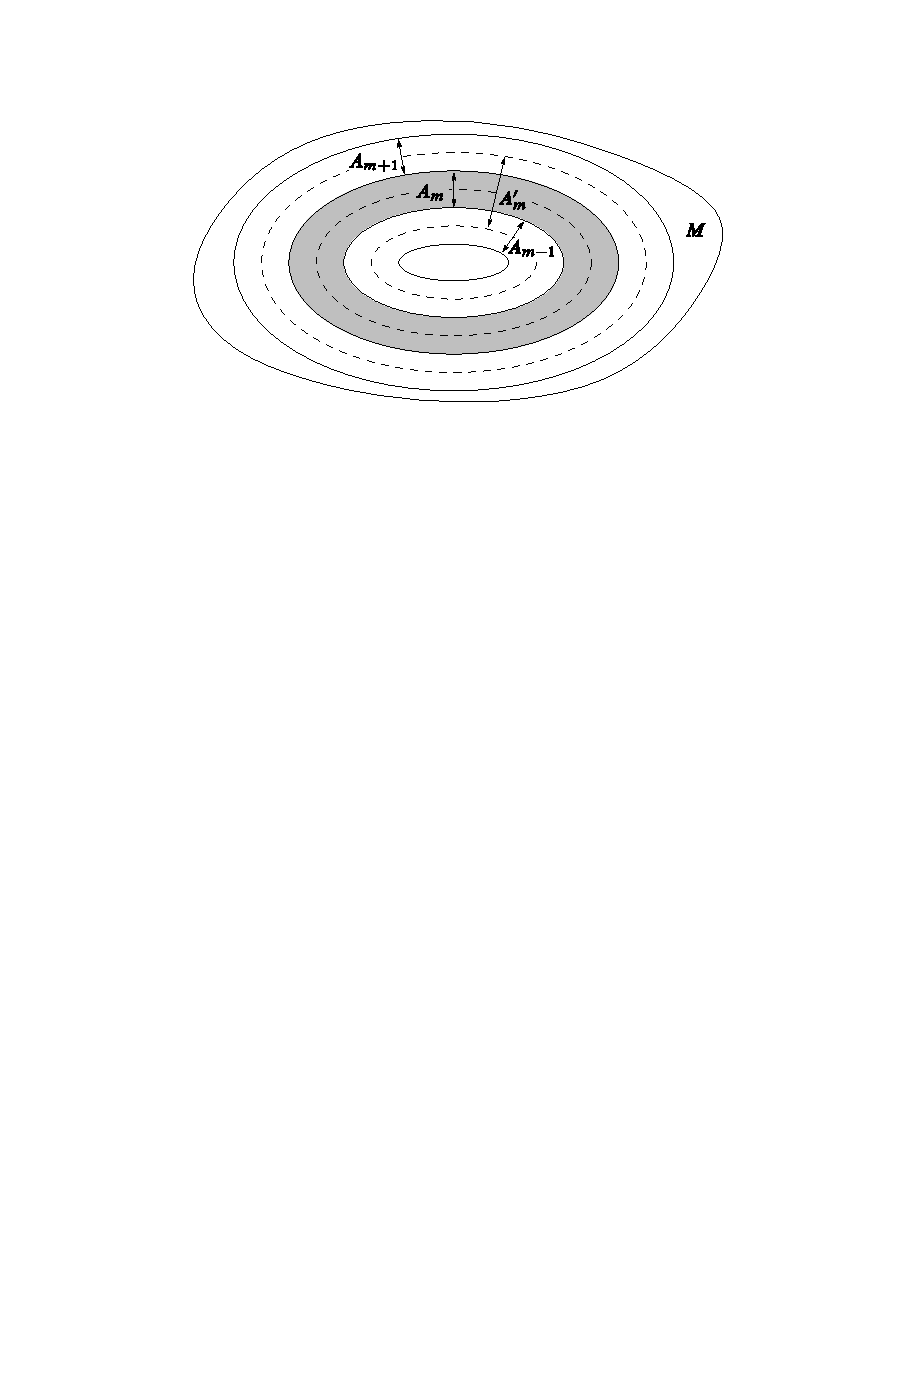
\includegraphics{pictures/induction-principle}
\caption{Proof of the induction principle, Step $2$.}
\end{figure}

Observe that $B_i\sub A'_i$, so $B_i$ can have nonempty intersection with $B_j$ only when $|i-j|\leq 1$. Therefore, if we define
\[U=\bigcup_{\text{$i$ odd}}B_i,\quad V=\bigcup_{\text{$i$ even}}B_i,\]
then $U$ and $V$ are disjoint unions of manifolds satisfying $\mathcal{P}$, and so they both satisfy $\mathcal{P}$ by condition (c). Finally, $\mathcal{P}$ holds on 
$U\cap V$ because it is the disjoint union of the sets $B_u\cap B_{i+1}$ for $i\in\Z$, each of which has a finite $\mathcal{P}$-cover consisting of sets of the form $U_\alpha\cap U_\beta$, 
where $U_\alpha$ and $U_\beta$ are basis sets used to define $B_i$ and $B_{i+1}$, respectively. Thus $M=U\cup V$ satisfies $\mathcal{P}$.\par
\textbf{Step $\bm{3}$}: Every open subset of $\R^n$ satisfies $\mathcal{P}$. If $U\sub\R^n$ is such a subset, then $U$ has a basis consisting of Euclidean cubes. 
Because each cube is diffeomorphic to $\R^n$, and because any finite intersection of cubes is again a cube, finite intersections also satisfies $\mathcal{P}$. Thus, 
$U$ has a $\mathcal{P}$-basis, so it satisfies $\mathcal{P}$ by Step $2$.\par
\textbf{Step $\bm{4}$}: Every smooth manifold satisfies $\mathcal{P}$. Any smooth manifold has a basis of smooth coordinate domains. Since every smooth coordinate 
domain is diffeomorphic to an open subset of $\R^n$, as are their finite intersections, this is a $\mathcal{P}$-basis. The claim therefore follows from Step $2$.
\end{proof}
The following lemma is needed in the proof of the Poincar\'e duality.
\begin{lemma}
The two Mayer-Vietoris sequences of the cover $\{U,V\}$ may be paired together to form a sign-commutative diagram
\[\begin{tikzcd}[row sep=14pt,column sep=14pt]
{}\ar[r]&H^p_{dR}(U\cup V)\ar[draw=none]{d}[name=X, anchor=center,scale=1.5]{\otimes}\ar[r,"\text{restriction}"]&H^p_{dR}(U)\oplus H^p_{dR}(V)\ar[draw=none]{d}[name=X, anchor=center,scale=1.5]{\otimes}
{}\ar[r,"\text{difference}"]&H^p_{dR}(U\cap V)\ar[draw=none]{d}[name=X, anchor=center,scale=1.5]{\otimes}\ar[r,"\delta^*"]&H^{p+1}(U\cup V)\ar[draw=none]{d}[name=X, anchor=center,scale=1.5]{\otimes}
\ar[r]&{}\\
{}&H_c^{n-p}(U\cup V)\ar[d,"\int_{U\cup V}"]\ar[l]&H_c^{n-p}(U)\oplus H^{n-p}_c(V)\ar[l,swap,"\text{sum}"]\ar[d,"\int_U+\int_V"]
&H^{n-p}_c(U\cap V)\ar[l]\ar[d,"\int_{U\cap V}"]&H_c^{n-p-1}(U\cup V)\ar[d,"\int_{U\cup V}"]\ar[l,swap,"\delta_*"]
&{}\ar[l]\\
&\R&\R&\R&\R&
\end{tikzcd}\]
\end{lemma}
Here sign-commutativity means, for instance, that
\[\int_{U\cap V}\omega\wedge\delta_*\eta=\pm\int_{U\cup V}\delta^*\omega\wedge\eta.\]
for $\omega\in H^p_{dR}(U\cap V)$, $\eta\in H^{n-p-1}_c(U\cup V)$.
\begin{proof}
The first two squares are in fact commutative: for $\omega\in H^p_{dR}(U\cup V)$ and $(\eta,\eta')\in H^{n-p}_c(U)\oplus H^{n-p}_c(V)$ we have
\[\int_{U\cup V}\omega\wedge\eta=\int_U\omega\wedge\eta,\quad \int_{U\cup V}\omega\wedge\eta=\int_V\omega\wedge\eta'\]
for $\eta$ is zero outside $U$ and $\eta'$ is zero outside $V$. Therefore
\[\int_{U\cup V}\omega\wedge(\eta+\eta')=\int_U\omega\wedge\eta+\int_V\omega\wedge\eta'.\]
which is the commutativity of the first squre. Similarly, for $(\omega,\omega')\in H^p_{dR}(U)\oplus H^p_{dR}(V)$ and $\eta\in H^{n-p}_c(U\cap V)$ we have
\[\int_{U}\omega\wedge\eta=\int_{U\cap V}\omega\wedge\eta,\quad \int_{U}\omega'\wedge\eta=\int_{U\cap V}\omega'\wedge\eta,\]
and therefore
\[\int_{U}\omega\wedge(-\eta)+\int_V\omega'\wedge\eta=\int_{U\cap V}(\omega-\omega')\wedge\eta,\]
which is the commutativity of the second squre.\par
The sign problem emerges on the third squre. Let $\omega\in H^p_{dR}(U\cap V)$ and $\eta\in H^{n-p-1}_c(U\cup V)$. Recall that $\delta^*\omega$ is a form in 
$H^{p+1}(U\cup V)$ such that
\[\delta^*\omega=\begin{cases}
d(\rho_V\omega)&\text{ on }U,\\
d(-\rho_U\omega)&\text{ on }V.
\end{cases}\]
Similaly, $\delta_*\eta$ is a form in $H^{n-p}_c(U\cap V)$ such that $\delta_*\eta=d(\rho_U\eta)$. Note that $d(\rho_U\eta)=(d\rho_U)\wedge\eta$ and 
$d(\rho_V\omega)=(d\rho_V)\wedge\omega$ because $\omega$ and $\eta$ are closed. Therefore
\[\int_{U\cap V}\omega\wedge\delta_*\eta=\int_{U\cap V}\omega\wedge(d\rho_U)\wedge\eta=(-1)^{\deg\omega}\int_{U\cap V}(d\rho_U)\wedge\omega\wedge\eta.\]
Since $\rho_U$ and $\rho_V$ are both constant outside $U\cap V$, we find that $\delta^*\omega$ has support in $U\cap V$, and therefore
\[\int_{U\cup V}\delta^*\omega\wedge\eta=\int_{U\cap V}d(\rho_V)\omega\wedge\eta=\int_{U\cap V}(d\rho_V)\wedge\omega\wedge\eta=-\int_{U\cap V}(d\rho_U)\wedge\omega\wedge\eta.\]
Thus finally we get
\[\int_{U\cap V}\omega\wedge\delta_*\eta=(-1)^{\det\omega+1}\int_{U\cup V}\delta^*\omega\wedge\eta.\]
This finishes the proof.
\end{proof}
\begin{proposition}[\textbf{Poincar\'e Duality}]
Let $M$ be an oriented manifold, then the pairing
\[\int:H^p_{dR}(M)\otimes H^{n-p}_c(M)\to\R\]
is nondegenerate. In particular, the two cohomology groups $H^p_{dR}(M)$ and $H^{n-p}_c(M)$ are dual to each other and therefore have the same dimension provided they are 
finite-dimensional vector spaces.
\end{proposition}
\begin{proof}
It is easy to see that the pairing is well-defined. Next note that it defines a
linear map
\[H^p_{dR}(M)\to H^{n-p}_c(M)^*=\Hom(H^{n-p}_c(M),\R).\]
We claim that this map is an isomorphism for all orientable but not necessarily connected
manifolds.\par
By the Five Lemma if Poincar\'e duality holds for $U$, $V$, and $U\cap V$, then it holds for $U\cup V$. We now proceed by checking the conditions in the induction principle. 
For $M$ diffeomorphic to $\R^n$, Poincar\'e duality follows from the two Poincar\'e lemmas. Next consider an arbitrary union of pairwise disjoint open sets. In this case we have
\[H^p_{dR}(\coprod_iU_i)=\prod_iH^p_{dR}(U_i)\quad H^{n-p}_c(\coprod_iU_i)=\bigoplus_iH^{n-p}_c(U_i).\]
so the claim also follows in this case. Then by Theorem the claim is valid for any oriented manifold.
\end{proof}
\begin{corollary}
Let $M$ be a compact oriented manifold. Then $H^p_{dR}(M)$ and $H^{n-p}_{dR}(M)$ are isomorphic.
\end{corollary}
\begin{proof}
This requires that we know that $H^p_{dR}(M)$ is finite dimensional for all $p$. First note that if $O\sub\R^n$ is a finite union of open boxes, then the de Rham cohomology 
groups are finite dimensional by the Mayer-Vietoris sequence.\par
This will give the result for $M\sub\R^k$ as we can find a tubular neighborhood $M\sub U\sub\R^k$ and a retract $r:U\to M$. Now cover $M$ by open boxes that lie in $U$ 
and use compactness of $M$ to find $M\sub O\sub U$ with $O$ being a union of finitely many open boxes. Since $r|_M=\id_M$ the retract $r^*:H^p_{dR}(M)\to H^p_{dR}(O)$ is 
an injection so it follows that $H^p_{dR}(M)$ is finite dimensional.
\end{proof}
\subsection{Cohomology computation on the top degree}
The Poincar\'e duality gives an easy way to compute the top cohomology for an manifolds. In this part we state the main results.
\begin{theorem}[\textbf{Top Cohomology, Orientable Compact Support Case}]\label{cohomology n orientable compact supp}
If $M$ is a connected orientable smooth $n$-manifold, then the integration map $\int:H^n_c(M)\to\R$ is an isomorphism, so $H^n_c(M)$ is $1$-dimensional.
\end{theorem}
\begin{proof}
This follows from the Poincar\'e duality, since $H^0_{dR}(M)$ consists of constant functions in this case.
\end{proof}
\begin{theorem}[\textbf{Top Cohomology, Orientable Compact Case}]\label{cohomology n orientable compact}
If $M$ is a compact connected orientable smooth $n$-manifold, then $H^n_{dR}(M)$ is $1$-dimensional, and is spanned by the cohomology class of any smooth orientation form.
\end{theorem}
\begin{proof}
This follows from the preceding theorem, because $H^p_{dR}(M)=H^p_c(M)$ in that case, and the integral of any orientation form is nonzero.
\end{proof}
\begin{theorem}[\textbf{Top Cohomology, Orientable Noncompact Case}]\label{cohomology n orientable noncompact}
If $M$ is a noncompact connected orientable smooth $n$-manifold, then $H^n_{dR}(M)=0$.
\end{theorem}
\begin{proof}
This also comes from the Poincar\'e duality: if $M$ is connected and noncompact, then $H^0_c(M)=0$.
\end{proof}
Next we consider the nonorientable case. If $M$ is a nonorientable smooth manifold, the key to analyzing its cohomology groups is the orientation covering $\widehat{\pi}:\widehat{M}\to M$. Because a finite-sheeted covering map is a proper map by Exercise~\ref{covering map proper iff}, $\widehat{\pi}$ induces cohomology maps on both compactly supported and ordinary de Rham cohomology. The next lemma shows that these maps are all injective.
\begin{lemma}
Suppose $M$ is a connected nonorientable smooth manifold and $\widehat{\pi}:\widehat{M}\to M$ is its orientation covering. For each $p$, the induced cohomology maps $\widehat{\pi}^*:H^p_{dR}(M)\to H^p_{dR}(\widehat{M})$ and $\widehat{\pi}^*:H^p_{c}(M)\to H^p_{c}(\widehat{M})$ are injective.
\end{lemma}
\begin{proof}
First, we prove the lemma for compactly supported cohomology. Suppose $\omega$ is a closed, compactly supported $p$-form on $M$ such that $\widehat{\pi}^*[\omega]=0\in H^p_c(\widehat{M})$. Then there exists $\eta\in\Omega^{p-1}_c(\widehat{M})$ such that $d\eta=\widehat{\pi}^*\omega$. Let $\alpha:\widehat{M}\to\widehat{M}$ be the unique nontrivial covering automorphism of $\widehat{M}$, and let $\widetilde{\eta}=\frac{1}{2}(\eta+\alpha^*\eta)$, which is also compactly supported. Using the fact that $\alpha\circ\alpha=\mathrm{id}_{\widehat{M}}$, we compute
\[\alpha^*\widetilde{\eta}=\frac{1}{2}(\alpha^*\eta+\alpha^*\circ\alpha^*\eta)=\widetilde{\eta}.\]
Because $\widehat{\pi}\circ\alpha=\widehat{\pi}$, this implies
\[d\widetilde{\eta}=\frac{1}{2}(d\eta+\alpha^*d\eta)=\frac{1}{2}(\widehat{\pi}^*\omega+\alpha^*\widehat{\pi}^*\omega)=\widehat{\pi}^*\omega.\]
Let $U\sub M$ be any evenly covered open subset. There are exactly two smooth local sections $\sigma_1,\sigma_2:U\to \widehat{M}$ over $U$, which are related by $\sigma_2=\alpha\circ\sigma_1$. Observe that
\[\sigma_2^*\widetilde{\eta}=\sigma_1^*\alpha^*\omega=\sigma_1^*\omega.\]
Therefore, we can define a smooth global $(p-1)$-form $\beta$ on $M$ by setting $\beta|_U:=\sigma^*\widetilde{\eta}$ for any smooth local section $\sigma:U\to\widehat{M}$; the argument above guarantees that the various definitions agree where they overlap. Because $\supp(\beta)=\widehat{\pi}(\supp(\widetilde{\eta}))$, it follows that $\beta$ is compactly supported. To determine the exterior derivative of $\beta$, given $p\in M$; choose a smooth local section $\sigma$ defined on a neighborhood $U$ of $p$, and compute
\[d\beta=d(\sigma^*\widetilde{\eta})=\sigma^*d\widetilde{\eta}=\sigma^*\widehat{\pi}^*\omega=\omega.\]
because $\widehat{\pi}\circ\sigma=\mathrm{id}_U$.\par
The argument for ordinary de Rham cohomology is the same, but with all references
to compact support deleted.
\end{proof}
\begin{theorem}[\textbf{Top Cohomology, Nonorientable Case}]\label{cohomology n nonorientable}
If $M$ is a connected nonorientable smooth $n$-manifold, then $H^n_c(M)=0$ and $H^n_{dR}(M)=0$.
\end{theorem}
\begin{proof}
First consider the case of compactly supported cohomology. By the preceding lemma, it suffices to show that $\widehat{\pi}^*:H^p_{c}(M)\to H^p_{c}(\widehat{M})$ is the zero map, where $\widehat{\pi}:\widehat{M}\to M$ is the orientation covering of $M$. Let $\alpha:\widehat{M}\to\widehat{M}$ be the nontrivial covering automorphism as in the preceding proof. Now, $\alpha$ cannot be orientation-preserving: if it were, the entire covering automorphism group $\{\mathrm{id},\alpha\}$ would be orientation-preserving, and then $M$ would be orientable by \cref{orientation covering thm}. By connectedness of $\widehat{M}$ and the fact that $\alpha$ is a diffeomorphism, it follows that $\alpha$ is orientation-reversing.\par
Suppose $\omega$ is any compactly supported smooth $n$-form on $M$, and let $\widehat{\omega}=\widehat{\pi}^*\omega$. Because $\widehat{\pi}$ is proper, $\widehat{\omega}$ is compactly supported, and $\widehat{\pi}\circ\alpha=\widehat{\pi}$ implies $\alpha^*\widehat{\omega}=\widehat{\omega}$. Because $\alpha$ is orientation-reversing, we conclude from \cref{int form prop} that
\[\int_{\widehat{M}}\widehat{\omega}=-\int_{\widehat{M}}\alpha^*\widehat{\omega}=-\int_{\widehat{M}}\widehat{\omega}.\]
This implies that $\int_{\widehat{M}}\widehat{\omega}=0$, so $[\widehat{\omega}]=0\in H^p_c(\widehat{M})$ by \cref{cohomology n orientable compact supp}. This completes the proof that $H^n_c(M)=0$.\par
It remains only to handle ordinary cohomology. If $M$ is compact, it follows from the argument above that $H^n_{dR}(M)=H^n_c(M)=0$. On the other hand, if $M$ is noncompact, then so is $\widehat{M}$, and \cref{cohomology n orientable noncompact} shows that $H^n_{dR}(\widehat{M})=0$. It follows from the previous lemma that $H^n_{dR}(M)=0$ as well.
\end{proof}
\subsection{Degree theory}
Now that we know the top-degree cohomology groups of all compact smooth manifolds, we can use them to draw a number of significant conclusions about smooth maps between certain compact manifolds of the same dimension. They all follow from the fact that we can associate an integer to each such map, called its degree, in
such a way that homotopic maps have the same degree.
\begin{theorem}[\textbf{Degree of a Smooth Map}]\label{degree def}
Suppose $M$ and $N$ are compact, connected, oriented, smooth manifolds of dimension $n$, and $F:M\to N$ is a smooth map. There exists a unique integer $k$, called the \textbf{degree of $\bm{F}$}, that satisfies both of the following conditions.
\begin{itemize}
\item[(a)] For every smooth $n$-form $\omega$ on $N$,
\[\int_MF^*\omega=k\int_N\omega.\]
\item[(b)] If $q\in N$ is a regular value of $F$, then
\[k=\sum_{x\in F^{-1}(q)}\sgn(x),\]
where $\sgn(x)=1$ if $dF_x$ is orientation-preserving, and $-1$ if it is orientation-reversing.
\end{itemize}
\end{theorem}
\begin{proof}
By \cref{cohomology n orientable compact}, two smooth $n$-forms on either $M$ or $N$ are cohomologous if and only if they have the same integral. Let $\theta$ be any smooth $n$-form on $N$ such that $\int_N\theta=1$, and let $k=\int_MF^*\theta$. If $\omega\in\Omega^n(N)$ is arbitrary, then $\omega$ is cohomologous to $a\theta$, where $a=\int_N\omega$, and therefore $F^*\omega$ is cohomologous to $aF^*\theta$. It follows that
\[\int_MF^*\omega=a\int_MF^*\theta=ak=k\int_N\omega.\]
Thus $k$ satisfies (a), and is clearly the only number that does so.\par
Next we show that $k$ also has the characterization given in part (b), from which it follows that it is an integer. Let $q\in N$ be an arbitrary regular value of $F$. Because $F^{-1}(q)$ is a properly embedded $0$-dimensional submanifold of $M$, it is finite. Suppose first that $F^{-1}(q)$ is not empty---say, $F^{-1}(q)=\{x_1,\dots,x_r\}$. By the inverse function theorem, for each $i$ there is a neighborhood $U_i$ of $x_i$ such that $F$ is a diffeomorphism from $U_i$ to a neighborhood $W_i$ of $q$, and by shrinking the $U_i$'s if necessary, we may assume that they are pairwise disjoint. Then $K:=M-\bigcup_{i=1}^{r}U_i$ is closed in $M$ and thus compact, so $F(K)$ is closed in $N$ and disjoint from $q$. Let $W$ be the connected component of $\bigcap_{i=1}^{r}W_i\cap(N-F(K))$ containing $q$, and let $V_i=F^{-1}(W)\cap U_i$. It follows that $W$ is a connected neighborhood of $q$ whose preimage under $F$ is the disjoint union $V_1\cup\cdots\cup V_r$, and $F$ restricts to a diffeomorphism from each $V_i$ to $W$. Since each $V_i$ is connected, the restriction of $F$ to $V_i$ must be either orientation-preserving or orientation-reversing.\par
Let $\omega$ be a smooth $n$-form on $N$ that is compactly supported in $W$ and satisfies $\int_N\omega=\int_W\omega=1$. It follows from part (a) that $\int_MF^*\omega=k$. Since $F^*\omega$ is compactly supported in $F^{-1}(W)$, we have $\int_MF^*\omega=\sum_{i=1}^{r}\int_{V_i}F^*\omega=k$. From \cref{int form prop}(d), since $F$ restricts to a diffeomorphism on each $V_i$, we conclude that $\int_{V_i}\omega=\pm 1$, with the positive sign if $F$ is orientation-preserving on $V_i$ and the negative sign otherwise. This proves (b) when $F^{-1}(q)\neq\emp$.\par
On the other hand, suppose $F^{-1}(q)=\emp$. Then $q$ has a neighborhood $W$ contained in $N-F(M)$ (because $F(M)$ is compact and thus closed). If $\omega$ is any smooth $n$-form on $N$ that is compactly supported in $W$, then $\int_MF^*\omega=0$, so $k=0$. This proves (b).
\end{proof}
\begin{corollary}
With the assumptions above, if $F$ is not surjective then $\deg F=0$.
\end{corollary}
Much of the power of degree theory arises from the fact that the two different characterizations of the degree can be played off against each other. For example, it is often easy to compute the degree of a particular map simply by counting the points in the preimage of a regular value, with appropriate signs. On the other hand, the characterization in terms of differential forms makes it easy to prove many important properties, such as the ones given in the next proposition.
\begin{proposition}[\textbf{Properties of the Degree}]\label{degree prop}
Suppose $M,N$, and $P$ are compact, connected, oriented, smooth $n$-manifolds.
\begin{itemize}
\item[(a)] If $F:M\to N$ and $G:N\to P$ are both smooth maps, then $\deg(G\circ F)=(\deg G)(\deg F)$.
\item[(b)] If $F:M\to N$ is a diffeomorphism, then $\deg F=+1$ if $F$ is orientation-preserving and $-1$ if it is orientation-reversing.
\item[(c)] If two smooth maps $F_0,F_1:M\to N$ are homotopic, then they have the same degree.
\end{itemize}
\end{proposition}
\begin{proof}
Part (b) and (c) follows directly from definition. For (a), we just note that
\[\int_P(G\circ F)^*\omega=\int_PF^*G^*\omega=(\deg F)\int_NG^*\omega=(\deg F)(\deg G)\int_M\omega,\]
which proves $\deg(G\circ F)=(\deg F)(\deg G)$.
\end{proof}
This proposition allows us to define the degree of a continuous map $F:M\to N$ between compact, connected, oriented, smooth $n$-manifolds, by letting $\deg F$ be the degree of any smooth map that is homotopic to $F$. The Whitney approximation theorem guarantees that there is such a map, and the preceding proposition guarantees that the degree is the same for every map homotopic to $F$. Here are some applications of degree theory.
\begin{proposition}
Let $F:M\to N$ be a proper local diffeomorphism of degree $\pm1$ between oriented connected manifolds, then $F$ is a diffeomorphism.
\end{proposition}
\begin{proof}
The fact that $\deg F\neq 0$ means $F$ is surjective, and thus a covering map. Now $\deg F=\pm 1$ means $F$ is injective, so it must be a diffeomorphism.
\end{proof}
\begin{proposition}
Even dimensional spheres do not admit non-vanishing smooth vector fields.
\end{proposition}
\begin{proof}
Let $X$ be a vector field on $S^n$, we can scale it so that it is a unit vector field. If we consider it as a function $X:S^n\to S^n\sub\R^{n+1}$ then it is always 
perpendicular to its foot point. We can then create a homotopy
\[H(p,t)=p\cos(\pi t)+X_p\sin(\pi t).\]
Since $p\bot X_p$ and both are unit vectors the Pythagorean theorem shows that $H(p,t)\in S^n$ as well. When $t=0$ the homotopy is the identity, and when $t=1$ it is the 
antipodal map. Since the antipodal map reverses orientations on even dimensional spheres it is not possible for the identity map to be homotopic to the antipodal map.
\end{proof}
\begin{theorem}
Suppose $N$ is a compact, connected, oriented, smooth $n$-manifold, and $X$ is a compact, oriented, smooth $(n+1)$-manifold with connected boundary. If $f:\partial X\to N$ is a continuous map that has a continuous extension to $X$, then $\deg f=0$.
\end{theorem}
\begin{proof}
Suppose $f$ has an extension to a continuous map $F:X\to N$. By the Whitney approximation theorem, there is a smooth map $\widetilde{F}:X\to N$ that is homotopic
to $F$. Replacing $F$ by $\widetilde{F}$ and $f$ by $\widetilde{F}|_{\partial X}$ we may assume that both $f$ and $F$ are smooth.\par
Let $\omega$ be any smooth $n$-form on $N$. Then $d\omega=0$ because it is an $(n+1)$-form on an $n$-manifold. From Stokes's theorem, we obtain
\[\int_{\partial X}f^*\omega=\int_{\partial X}F^*\omega=\int_Xd(F^*\omega)=\int_XF^*(f\omega)=0.\]
It follows from \cref{degree def} that $f$ has degree zero.
\end{proof}
\begin{theorem}[\textbf{Brouwer Fixed-Point Theorem}]
Every continuous map from $\widebar{B}^n$ to itself has a fixed point.
\end{theorem}
\begin{proof}
Suppose for the sake of contradiction that $F:\widebar{B}^n\to\widebar{B}^n$ is continuous and has no fixed points. We can define a continuous map
\[G(x)=\frac{x-F(x)}{|x-F(x)|},\]
and let $g=G|_{S^{n-1}}:S^{n-1}\to S^{n-1}$. On the one hand, the previous theorem implies that $g$ has degree zero. On the other hand, consider the map 
$H:S^{n-1}\times I\to S^{n-1}$ defined by
\[H(x,t)=\frac{x-tF(x)}{|x-tF(x)|}\]
The denominator never vanishes when $t=1$ because $F$ has no fixed points, and when $t<1$ it cannot vanish because $|x|=1$ while $|tF(x)|=t<1$. Thus $H$ is continuous, 
so it is a homotopy from the identity to $g$. It follows from \cref{degree prop} that $g$ has degree $1$, which is a contradiction.
\end{proof}
\subsection{The de Rham theorem}
The topological invariance of the de Rham groups suggests that there should be some purely topological way of computing them. There is indeed, and the connection 
between the de Rham groups and the singular cohomology groups was first proved by Georges de Rham himself in the 1930s. The theorem that bears his name is a major 
landmark in the development of smooth manifold theory. The purpose of this part is to give a proof of this theorem.
\paragraph{Smooth singular homology}
The connection between the singular and de Rham cohomology groups will be established by integrating differential forms over singular chains. More precisely, given a 
singular $p$-simplex $\sigma$ in a manifold $M$ and a $p$-form $\omega$ on $M$, we would like to pull $\omega$ back by $\sigma$ and integrate the resulting form over 
$\Delta_p$. However, there is an immediate problem with this approach, because forms can be pulled back only by smooth maps, while singular simplices are in general 
only continuous. In this part we overcome this problem by showing that singular homology can be computed equally well with smooth simplices.\par
If $M$ is a smooth manifold, a smooth $p$-simplex in $M$ is a map $\sigma:\Delta_p\to M$ that is smooth in the sense that it has a smooth extension to a neighborhood 
of each point. The subgroup of $C_p(M)$ generated by smooth simplices is denoted by $C^\infty_p(M)$ and called the \textbf{smooth chain group in degree $\bm{p}$}. 
Elements of this group, which are finite formal linear combinations of smooth simplices, are called smooth chains. Because the boundary of a smooth simplex is a smooth 
chain, we can define the \textbf{$\bm{p}$-th smooth singular homology group} of $M$ to be the quotient group
\[H_p^{\infty}(M)=\frac{\ker(\partial:C_p^{\infty}(M)\to C_{p-1}^{\infty}(M))}{\im(\partial:C_{p+1}^{\infty}(M)\to C_{p}^{\infty}(M))}.\]
The inclusion map $\iota:C^\infty_p(M)\hookrightarrow C_p(M)$ commutes with the boundary operator, and so induces a map on homology: $\iota_*:H_p^{\infty}(M)\to H_p(M)$ 
by $\iota_*[c]=[\iota(c)]$.
\begin{theorem}[\textbf{Smooth Singular vs. Singular Homology}]
For any smooth manifold $M$, the map $\iota_*:H_p^{\infty}(M)\to H_p(M)$ induced by inclusion is an isomorphism.
\end{theorem}
The basic idea of the proof is to construct, with the help of the Whitney approximation theorem, two operators: first, a smoothing operator $s:C_p(M)\to C_p^{\infty}(M)$ 
such that $s\circ\partial=\partial\circ s$ and $s\circ\iota$ is the identity on $C_p^{\infty}(M)$; and second, a homotopy operator that shows that $\iota\circ s$ induces 
the identity map on $H^p(M)$. Since the details are highly technical, we do not present them here.
\paragraph{The de Rham theorem}
Suppose $M$ is a smooth manifold, $\omega$ is a closed $p$-form on $M$; and $\sigma$ is a smooth $p$-simplex in $M$. We define the integral of $\omega$ over $\sigma$ to 
be
\[\int_{\sigma}\omega=\int_{\Delta_p}\sigma^*\omega.\]
This makes sense because $\Delta_p$ is a smooth $p$-submanifold with corners embedded in $\R^p$, and it inherits the orientation of $\R^p$. (Or we could just consider $\Delta_p$ 
as a domain of integration in $\R^p$.) Observe that when $p=1$, this is the same as the line integral of $\omega$ over the smooth curve segment $\sigma:[0,1]\to M$. If 
$c=\sum_{i=1}^{k}c_i\sigma_i$ is a smooth $p$-chain, the integral of $\omega$ over $c$ is defined as
\[\int_{c}\omega=\sum_{i=1}^{k}c_i\int_{\sigma_i}\omega.\]
\begin{theorem}[\textbf{Stokes's Theorem for Chains}]\label{Stokes's theorem for chains}
If $c$ is a smooth $p$-chain in a smooth manifold $M$, and $\omega$ is a smooth $(p-1)$-form on $M$, then
\[\int_cd\omega=\int_{\partial c}\omega.\]
\end{theorem}
\begin{proof}
It suffices to prove the theorem when $c$ is just a smooth simplex $\sigma$. Since $\Delta_p$ is a manifold with corners, Stokes's theorem says that
\[\int_{\sigma}d\omega=\int_{\Delta_p}\sigma^*d\omega=\int_{\Delta_p}d\sigma^*\omega=\int_{\partial\Delta_p}\sigma^*\omega.\]
The face maps $F_{i,p}:\Delta_{p-1}\to\Delta_p$ are parametrizations of the boundary faces of $\Delta_p$ satisfying the conditions of \cref{int mani para}, 
except possibly that they might not be orientation-preserving. To check the orientations, note that $F_{i,p}$ is the restriction to $\Delta_p\cap\partial\H^p$ of the 
affine diffeomorphism sending the simplex $[e_0,\dots,e_p]$ to $[e_0,\dots,\widehat{e}_i,\dots,e_p,e_i]$. This is easily seen to be orientation-preserving if and only 
if $(e_0,\dots,\widehat{e}_i,\dots,e_p,e_i)$ is an even permutation of $(e_0,\dots,e_p)$, which is the case if and only if $p-i$ is even. Since the standard coordinates 
on $\partial\H^p$ are positively oriented if and only if $p$ is even, the upshot is that $F_{i,p}$ is orientation-preserving for $\partial\Delta_p$ if and only if $i$ is 
even. Thus, by \cref{int mani para},
\begin{align*}
\int_{\partial\Delta_p}\sigma^*\omega&=\sum_{i=0}^{p}(-1)^i\int_{\Delta_{p-1}}F_{i,p}^*\sigma^*\omega=\sum_{i=0}^{p}(-1)^i\int_{\Delta_{p-1}}(\sigma\circ F_{i,p})^*\omega=\sum_{i=0}^{p}(-1)^i\int_{\sigma\circ F_{i,p}}\omega.
\end{align*}
By definition of the singular boundary operator, this is equal $\int_{\partial\sigma}\omega$.
\end{proof}
Using this theorem, we define a natural linear map $\mathscr{I}:H_{dR}^p(M)\to H^p(M;\R)$, called the \textbf{de Rham homomorphism}, as follows. For any $[\omega]\in H^p_{dR}(M)$ 
and $[c]\in H_p(M)\cong H_p^{\infty}(M)$, we define
\[\mathscr{I}[\omega][c]=\int_{\widetilde{c}}\omega.\]
where $\widetilde{c}$ is any smooth $p$-cycle representing the homology class $[c]$. This is well defined by \cref{Stokes's theorem for chains}.
\begin{proposition}[\textbf{Naturality of the de Rham Homomorphism}]\label{de Rham homomorphism naturality}
For a smooth manifold $M$ and nonnegative integer $p$, let $\mathscr{I}:H^p_{dR}(M)\to H^p(M;\R)$ denote the de Rham homomorphism.
\begin{itemize}
\item[(a)] If $F:M\to N$ is a smooth map, then the following diagram commutes:
\[\begin{tikzcd}[row sep=12pt,column sep=12pt]
H_{dR}^p(N)\ar[r,"F^*"]\ar[d,"\mathscr{I}"]&H_{dR}^p(M)\ar[d,"\mathscr{I}"]\\
H^p(N;\R)\ar[r,"F^*"]&H^p(M;\R)
\end{tikzcd}\] 
\item[(b)] If $M$ is a smooth manifold and $U,V$ are open subsets of $M$ whose union is $M$, then the following diagram commutes:
\[
\begin{tikzcd}[row sep=12pt,column sep=12pt]
H_{dR}^{p-1}(U\cap V)\ar[r,"\delta"]\ar[d,"\mathscr{I}"]&H_{dR}^p(M)\ar[d,"\mathscr{I}"]\\
H^{p-1}(U\cap V;\R)\ar[r,"\partial^*"]&H^{ppp}(M;\R)
\end{tikzcd}
\]
where $\delta$ and $\partial^*$ are the connecting homomorphisms of the Mayer-Vietoris sequences for de Rham and singular cohomology, respectively.
\end{itemize}
\end{proposition}
\begin{proof}
Directly from the definitions, if $\sigma$ is a smooth $p$-simplex in $M$ and $\omega$ is a smooth $p$-form on $N$,
\[\int_{\sigma}F^*\omega=\int_{\Delta_p}\sigma^*F^*\omega=\int_{\Delta_p}(F\circ\sigma)^*\omega=\int_{F\circ\sigma}\omega.\]
This implies
\[\mathscr{I}[F^*\omega][\sigma]=\mathscr{I}[\omega][F\circ\sigma]=F^*(\mathscr{I}[\omega])[\sigma].\]
which proves (a).\par
Now consider (b). Commutativity of this diagram means
\[\mathscr{I}(\delta[\omega])[e]=(\partial^*\mathscr{I}[\omega])[e]\]
for any $[\omega]\in H^{p-1}_{dR}(U\cap V)$ and any $[e]\in H^p_{dR}(M)$. Using our identification of $H^p(M;\R)$ with $\Hom(H^p(M),\R)$, we can rewrite this as
\[\mathscr{I}(\delta[\omega])[e]=\mathscr{I}[\omega](\partial_*[e]).\]
If $\sigma$ is a smooth $p$-form representing $\delta[\omega]$ and $c$ is a smooth $(p-1)$-chain representing $\partial_*[e]$, this is the same as 
\[\int_e\sigma=\int_c\omega.\]
By the characterization of $\partial_*$, we can let $c=\partial f$, where $f,f'$ are smooth $p$-chains in $U$ and $V$, respectively, such that $f+f'$ represents the 
same homology class as $e$. Similarly, by \cref{Mayer-Vietoris de Rham connect}, we can choose $\eta\in\Omega^{p-1}(U)$ and $\eta'\in\Omega^{p-1}(V)$ such that $\omega=\eta|_{U\cap V}-\eta'|_{U\cap V}$, 
and then let $\sigma$ be the $p$-form that is equal to $d\eta$ on $U$ and to $d\eta'$ on $V$. Then, because $\partial f+\partial f'=\partial e=0$ and $d\eta|_{U\cap V}-d\eta'|_{U\cap V}=d\omega=0$, 
we have
\begin{align*}
\int_{c}\omega&=\int_{\partial f}\omega=\int_{\partial f}\eta-\int_{\partial f}\eta'=\int_{\partial f}\eta+\int_{\partial f'}\eta'\\
&=\int_{f}d\eta+\int_{f'}d\eta'=\int_f\sigma+\int_{f'}\sigma=\int_{e}\sigma.
\end{align*}
Thus the diagram commutes.
\end{proof}
\begin{theorem}[\textbf{de Rham}]
For every smooth manifold $M$ and nonnegative integer $p$, the de Rham homomorphism $\mathscr{I}:H^p_{dR}(M)\to H^p(M;\R)$ is an isomorphism.
\end{theorem}
\begin{proof}
We will use the induction principle as in the proof of Poincar\'e duality. Thus we need to check the three conditions.\par
Consider $\R^n$. The homopoty invariant of $H^p$ implies that the singular cohomology groups of $\R^n$ are also trivial for $p\neq 0$. In the $p=0$ case, $H^0_{dR}(\R^n)$ 
is the $1$-dimensional space consisting of the constant functions, and $H^0(\R^n;\R)=\Hom(H_0(\R^n),\R)$ is also $1$-dimensional because $H_0(\R^n)$ is generated by any 
singular $0$-simplex. If $\sigma:\Delta_0\to M$ is a singular $0$-simplex (which is smooth because any map from a $0$-manifold is smooth), and $f$ is the constant function 
equal to $1$, then
\[\mathscr{I}[f][\sigma]=\int_{\Delta_0}\sigma^*f=(f\circ\sigma)(0)=1.\]
Thus $\mathscr{I}:H^0_{dR}(\R^n)\to H^0(\R^n;\R)$ is not the zero map, so it is an isomorphism.\par
If $U,V$ are open subsets of $M$ such that the de Rham theorem is true on $U$, $V$ and $U\cap V$, then putting together the Mayer-Vietoris sequences for de Rham and 
singular cohomology, we obtain the following commutative diagram, in which the horizontal rows are exact and the vertical maps are all de Rham homomorphisms:
\[\begin{tikzcd}[scale=0.85]
H_{dR}^{p-1}(U)\oplus H_{dR}^{p-1}(V)\ar[r]\ar[d]&H^{p-1}_{dR}(U\cup V)\ar[r]\ar[d]&H^p_{dR}(U\cup V)\ar[r]\ar[d]&H^p_{dR}(U)\oplus H^p_{dR}(V)\ar[d]\\
H^{p-1}(U;\R)\oplus H^{p-1}(V;\R)\ar[r]&H^{p-1}(U\cup V;\R)\ar[r]&H^p(U\cup V;\R)\ar[r]&H^p(U;\R)\oplus H^p(V;\R)
\end{tikzcd}\]
The commutativity of the diagram is an immediate consequence of \cref{de Rham homomorphism naturality}. Then by the five lemma the de Rham theorem is true on 
$U\cup V$.\par
Finally, consider a disjoint union $\amalg_iU_i$. For both de Rham and singular cohomology the inclusions $\iota_i:U_i\hookrightarrow\amalg_iU_i$ induce isomorphisms 
between the cohomology groups of the disjoint union and the direct product of the cohomology groups of the manifolds $U_i$. By \cref{de Rham homomorphism naturality}, 
$\mathscr{I}$ commutes with these isomorphisms. Now use the induction principal we get the claim.
\end{proof}
Recall that by \cref{homotopy equiv Int M to M} the inclusion $\iota:\Int M\hookrightarrow M$ is a homotopy equivalence, so for manifolds with boundary the de Rham theorem also holds.
\begin{proposition}
For every smooth manifold with boundary $M$ and nonnegative integer $p$, the de Rham homomorphism $\mathscr{I}:H^p_{dR}(M)\to H^p(M;\R)$ is an isomorphism.
\end{proposition}
\subsection{The Thom isomorphism}
\paragraph{Compact vertical cohomology and integration along the fiber}
For vector bundles there is a third kind of cohomology. Instead of $\Omega^p_c(E)$, the complex of forms with compact support, we consider $\Omega_{cv}^p(E)$, the 
complex of forms with compact support in the vertical direction, defined as follows: a smooth $n$-form $\omega$ on $E$ is in $\Omega^p_{cv}(E)$ if and only if for 
every compact set $K$ in $M$, $\supp(\omega)\cap\pi^{-1}(K)$ is compact. If $\omega\in\Omega^p_{cv}(E)$, then since $\supp(\omega|_{\pi^{-1}(p)})\sub\supp(\omega)\cap\pi^{-1}(p)$ 
is a  closed subset of a compact set, $\supp(\omega|_{\pi^{-1}(p)})$ is compact. Thus, although a form in $\Omega^p_{cv}(E)$ need not have compact support in $E$, its 
restriction to each fiber has compact support. The cohomology of this complex, denoted $\Omega^p_{cv}(E)$, is called the \textbf{cohomology of $\bm{E}$ with compact 
support in the vertical direction}, or \textbf{compact vertical cohomology}.\par
Let $E$ be oriented as a rank $k$ vector bundle. We define the \textbf{integration along the fiber}, $\Omega^p_{cv}(E)\to\Omega^{p-k}(M)$, as follows. First consider 
the case of a trivial bundle $E=M\times\R^n$. Let $(t^1,\dots,t^k)$ be the coordinates on the fiber $\R^k$. A form on $E$ is a real linear combination of two types of 
forms: the type (\rmnum{1}) forms are those which do not contain as a factor the $k$-form $dt_1\wedge\cdots\wedge dt_k$ and the type (\rmnum{2}) forms are those which 
do. The map $\pi_*$ is defined by
\begin{itemize}
\item[(\rmnum{1})] $(\pi^*\phi)\wedge f(x,t)\,dt^{i_1}\wedge\cdots\wedge dt^{i_r}\mapsto 0$, $r<k$.
\item[(\rmnum{2})] $(\pi^*\phi)\wedge f(x,t)\,dt^{1}\wedge\cdots\wedge dt^{k}\mapsto \phi\int_{\R^k}f(x,t)\,dt^1\wedge\cdots\wedge dt^k$.
\end{itemize}
where $f$ has compact support for each fixed $x$ in $M$ and $\phi$ is a form on $M$.\par
Next suppose $E$ is an oriented vector bundle, with oriented trivialization $\{(U_\alpha,\varPhi_\alpha)\}$. Let $(x^1,\dots,x^n)$ and $(\widetilde{x}^1,\dots,\widetilde{x}^n)$ 
be the coordinate functions on $U_\alpha$ and $U_\beta$ and $(t^1,\dots,t^k)$, $(\widetilde{t}^1,\dots,\widetilde{t}^k)$ the fiber coordinates on $E|_{U_\alpha}$ and 
$E|_{U_\beta}$, given by $\varPhi_\alpha$, $\varPhi_{\beta}$ respectively. Because $\{(U_\alpha,\varPhi_\alpha)\}$ is an oriented trivialization for $E$, the two sets 
of fiber coordinates $(t^1,\dots,t^k)$ and $(\widetilde{t}^1,\dots,\widetilde{t}^k)$ are related by an element of $\GL_n^+(\R)$ at each point of $U_\alpha\cap U_\beta$. 
Again a form $\omega$ in $\Omega_{cv}^p(E)$ is locally of type (\rmnum{1}) or (\rmnum{2}). The map $\pi_*$ is defined to be zero on type (\rmnum{1}) forms. To define $\pi_*$ on type (\rmnum{2}) forms, write $\omega_\alpha$ for $\omega|_{U_\alpha}$. Then
\[\omega_\alpha=(\pi^*\phi)\wedge f(x,t)\,dt^1\wedge\cdots\wedge dt^k,\quad \omega_\beta=(\pi^*\tau)\wedge g(\widetilde{x},\widetilde{t})\,d\widetilde{t}^1\wedge\cdots\wedge d\widetilde{t}_k.\]
Define
\[\pi_*\omega_\alpha=\phi\int_{\R^k}f(x,t)\, dt^1\wedge\cdots\wedge dt^k.\]
By the invariance of the integral under orientation-preserving diffeomorphism, these definitions coincide on their overlap. Hence $\{\omega_\alpha\}$ piece together to give a global form $\pi_*\omega$ on $M$. Furthermore, this definition is independent of the choice of the oriented trivialization for $E$.
\begin{proposition}
Integration along the fiber commutes with exterior differentiation.
\end{proposition}
\begin{proof}
By a partition of unity, we may assume $E$ to be the product bundle $M\times\R^k$. If $\omega=(\pi^*\phi)\wedge f(x,t)\,dt^1\wedge\cdots\wedge dt^k$, then we have
\begin{equation*}
\scalemath{0.9}{
\begin{aligned}
d(\pi_*\omega)&=d(\phi\int_{\R^k}f(x,t)\,dt_1\wedge\cdots\wedge dt_k)\\
&=(d\phi)\int_{\R^k}f(x,t)\,dt^1\wedge\cdots\wedge dt^k+(-1)^{\deg\phi}\phi\wedge \Big(d\int_{\R^k}f(x,t)\,dt^1\wedge\cdots\wedge dt^k\Big)\\
&=(d\phi)\int_{\R^k}f(x,t)\,dt^1\wedge\cdots\wedge dt^k+(-1)^{\deg\phi}\phi\wedge \Big(\int_{\R^k}\sum_{i=1}^{n}\frac{\partial f}{\partial x^i}(x,t)dx^i\wedge dt^1\wedge\cdots\wedge dt^k\\
&\quad +\int_{\R^k}\sum_{j=1}^{k}\frac{\partial f}{\partial t^i}(x,t)dt^j\wedge dt^1\wedge\cdots\wedge dt^k\Big)\\
&=(d\phi)\int_{\R^k}f(x,t)\,dt^1\wedge\cdots\wedge dt^k+(-1)^{\deg\phi}\phi\wedge dx^i\int_{\R^k}\sum_{i=1}^{n}\frac{\partial f}{\partial x^i}(x,t)\,dt^1\wedge\cdots\wedge dt^k.
\end{aligned}}
\end{equation*}
And
\begin{equation*}
\scalemath{0.9}{
\begin{aligned}
\pi_*(d\omega)&=\pi_*\Big((\pi^*d\phi)\wedge f(x,t)\,dt^1\wedge\cdots\wedge dt^k+\sum_i(-1)^{\deg\phi}(\pi^*\phi)\wedge\frac{\partial f}{\partial x^i}dx^i\wedge dt^1\wedge\cdots\wedge dt^k\Big)\\
&=\pi_*\Big((\pi^*d\phi)\wedge f(x,t)\,dt^1\wedge\cdots\wedge dt^k+\pi^*\Big(\sum_i(-1)^{\deg\phi}\phi\wedge dx^i\Big)\wedge\frac{\partial f}{\partial x^i}dx^i\wedge dt^1\wedge\cdots\wedge dt^k\Big)\\
&=(d\phi)\int_{\R^k}f(x,t)\,dt^1\wedge\cdots\wedge dt^k+(-1)^{\deg\phi}\phi\wedge dx^i\int_{\R^k}\sum_{i=1}^{n}\frac{\partial f}{\partial x^i}(x,t)\,dt^1\wedge\cdots\wedge dt^k.
\end{aligned}}
\end{equation*}
So $d\pi_*=\pi_*d$ for a type (\rmnum{2}) form. Next let $\omega=(\pi^*\phi)\wedge f(x,t)\,dt^{i_1}\wedge\cdots\wedge dt^{i_r}$, $r<k$, be a type (\rmnum{1}) form. Then $d\pi_*\omega=0$, and 
\begin{align*}
d\omega&=(\pi^*d\phi)\wedge f(x,t)\,dt^{i_1}\wedge\cdots\wedge dt^{i_r}+\pi^*\Big(\sum_{i=1}^{k}(-1)^{\deg\phi}\phi\wedge dx^i\Big)\wedge\frac{\partial f}{\partial x^i}(x,t)\,dt^{i_1}\wedge\cdots\wedge dt^{i_r}\\
&\quad+(\pi^*\phi)\wedge\Big(\sum_{j=1}^{k}(-1)^{\deg\phi}\frac{\partial f}{\partial t^j}(x,t)\,dt^j\wedge dt^{i_1}\wedge\cdots\wedge dt^{i_r}\Big)
\end{align*}
and so 
\begin{align*}
\pi_*(d\omega)&=\sum_{j=1}^{k}(-1)^{\deg\phi}\phi\int_{\R^k}\frac{\partial f}{\partial t^j}(x,t)\,dt^j\wedge dt^{i_1}\wedge\cdots\wedge dt^{i_r}\\
&=0\text{ if $dt^j\wedge dt^{i_1}\wedge\cdots dt^{i_r}\neq\pm dt^1\wedge\cdots\wedge dt^k$.}
\end{align*}
If $dt^j\wedge dt^{i_1}\wedge\cdots dt^{i_r}=\pm dt^1\wedge\cdots\wedge dt^k$, then $\int_{\R^k}\partial f/\partial t^j(x,t)\,dt^j\wedge dt^{i_1}\wedge\cdots\wedge dt^{i_r}$ is again 0: 
because $f$ has compact support,
\[\int_{\R}\frac{\partial f}{\partial t^j}(x,t)dt^j=0.\]
This completes the proof.
\end{proof}
Note that integration along the fiber lowers the degree of a form by the fiber dimension.
\begin{lemma}
An orientable vector bundle $E$ over an orientable manifold $M$ is an orientable manifold.
\end{lemma}
\begin{proof}
This follows from the fact that if $\{(U_\alpha,\varphi_\alpha)\}$ is an oriented atlas for $M$ with transition functions $\rho_{\alpha\beta}=\varphi_\alpha\circ\varphi_\beta^{-1}$ 
and $\varPhi_\alpha:\pi^{-1}(U_\alpha)\to U_\alpha\times\R^k$ is a local trivialization for $E$ with transition functions $\{\tau_{\alpha\beta}\}$ then the composition
\[\begin{tikzcd}
\pi^{-1}(U_\alpha)\ar[r,"\varPhi_\alpha"]&U_\alpha\times\R^k\ar[r,"\varphi_\alpha\times\id_{\R^k}"]&\R^{n}\times\R^k
\end{tikzcd}\]
gives an atlas for $E$. The typical transition function of this atlas,
\[(\varphi_\alpha\times\id_{\R^k})\circ\varPhi_\alpha\circ\varPhi_\beta^{-1}\circ(\varphi_\beta\times\id_{\R^k})^{-1}:\R^n\times\R^k\to\R^n\times\R^k\]
sends $(x,y)$ to $(\rho_{\alpha\beta}(x),\tau_{\alpha\beta}(\varphi_{\beta}^{-1}(x))y)$ and has Jacobian matrix
\[\begin{pmatrix}
\partial(\rho_{\alpha\beta})&0\\
*&\tau_{\alpha\beta}(\varphi_{\beta}^{-1}(x))
\end{pmatrix}\]
The determinant of this matrix is clearly positive.
\end{proof}
\begin{remark}
The orientation on $E$ described above is called the \textbf{local product orientation} on $E$.
\end{remark}

\begin{proposition}[\textbf{Projection Formula}]
Let $\pi:E\to M$ be an oriented rank $k$ vector bundle, $\pi_*:\Omega^p_{cv}(E)\to\Omega^{p-k}(M)$ be the integration along the fiber defined above.
\begin{itemize}
\item[(a)] Let $\tau$ be a form on $M$ and $\omega$ a form on $E$ with compact support along the fiber. Then
\[\pi_*((\pi^*\tau)\wedge\omega)=\tau\wedge\pi_*\omega.\] 
\item[(b)] Suppose in addition that $M$ is oriented of dimension $n$, $\omega\in\Omega^p_{cv}(E)$, and $\tau\in\Omega^{n+k-p}_c(M)$. Then with the local product 
orientation on $E$,
\begin{align}\label{de Rham int on fiber projection formula-1}
\int_E(\pi^*\tau)\wedge\omega=\int_M\tau\wedge\pi_*\omega.
\end{align}
\end{itemize}
\end{proposition}
\begin{proof}
By a partition of unity we may assume that $E$ is the product bundle $M\times\R^n$. If $\omega$ is a form of type (\rmnum{1}), say $\omega=(\pi^*\phi)\wedge f(x,t)\,dt^{i_1}\wedge\cdots\wedge dt^{i_r}$, 
where $r<k$, then
\begin{align*}
\pi_*((\pi^*\tau)\wedge\omega)&=\pi_*((\pi^*\tau)\wedge(\pi^*\phi)\wedge f(x,t)\,dt^{i_1}\wedge\cdots\wedge dt^{i_r})\\
&=\pi_*(\pi^*(\tau\wedge\phi)\wedge f(x,t)\,dt^{i_1}\wedge\cdots\wedge dt^{i_r})=0\\
&=\tau\wedge\pi_*\omega.
\end{align*}
If $\omega$ is a form of type (\rmnum{2}), say $\omega=(\pi^*\phi)\wedge f(x,t)\,dt^{1}\wedge\cdots\wedge dt^{n}$, then
\begin{align*}
\pi_*((\pi^*\tau)\wedge\omega)&=\pi_*((\pi^*\tau)\wedge(\pi^*\phi)\wedge f(x,t)\,dt^{1}\wedge\cdots\wedge dt^{n})\\
&=\tau\wedge\phi\int_{\R^k}f(x,t)\,dt^{1}\wedge\cdots\wedge dt^{n}\\
&=\tau\wedge\pi_*\omega.
\end{align*}
This proves (a).\par
For (b), if $\omega=(\pi^*\phi)\wedge f(x,t)\,dt^{i_1}\wedge\cdots\wedge dt^{i_r}$ with $r<k$, then by dimension consideration we have $(\pi^*\tau)\wedge(\pi^*\phi)=0$, 
so both sides of $(\ref{de Rham int on fiber projection formula-1})$ are zero. On the other hand, if $\omega=(\pi^*\phi)\wedge f(x,t)\,dt^{1}\wedge\cdots\wedge dt^{k}$, then
\begin{align*}
\int_E(\pi^*\tau)\wedge\omega&=\int_{M\times\R^k}\pi^*(\tau\wedge\phi)\wedge f(x,t)\,dt^1\wedge\cdots\wedge dt^k\\
&=\int_M\tau\wedge\phi\wedge\int_{\R^k}f(x,t)\,dt^1\wedge\cdots\wedge dt^k\\
&=\int_M\tau\wedge\pi_*\omega.
\end{align*}
This gives (b).
\end{proof}
Now we will show that integration along the fiber induces an isomorphism on cohomology groups. To use the induction principle, we first deal with the case $M=\R^n$. But 
in fact we have the following stronger result.
\begin{proposition}[\textbf{Poincar\'e Lemma for Compact Vertical Supports}]
Integration along the fiber defines an isomorphism
\[\pi_*:H^*_{cv}(M\times\R^k)\to H^{*-k}(M).\]
\end{proposition}
\begin{theorem}[\textbf{Thom Isomorhism}]\label{Thom iso}
If the vector bundle $\pi:E\to M$ over a manifold $M$ is orientable, then
\[H^*_{cv}(E)\cong H^{*-k}(M)\]
where $k$ is the rank of $E$.
\end{theorem}
\begin{proof}
Let $U$ and $V$ be open subsets of $M$. Using a partition of unity from the base $M$ we see that
\[\begin{tikzcd}
0\ar[r]&\Omega^*_{cv}(E|_{U\cup V})\ar[r]&\Omega^*_{cv}(E|_{U})\oplus\Omega^*_{cv}(E|_{V})\ar[r]&\Omega^*_{cv}(E|_{U\cap V})\ar[r]&0
\end{tikzcd}\]
is exact. So we have the diagram of Mayer-Vietoris sequences
\[\begin{tikzcd}[scale=0.75]
\cdots\ar[r]&H^p_{cv}(E|_{U\cup V})\ar[r]\ar[d,"\pi_*"]&H^p_{cv}(E|_{U})\oplus H^p_{cv}(E|_{V})\ar[r]\ar[d,"\pi_*"]&H^p_{cv}(E|_{U\cap V})\ar[r,"\delta^*"]\ar[d,"\pi_*"]&H^{p+1}_{cv}(E|_{U\cup V})\ar[r]\ar[d,"\pi_*"]&\cdots\\
\cdots\ar[r]&H^{p-k}(U\cup V)\ar[r]&H^{p-k}(U)\oplus H^{p-k}(V)\ar[r]&H^{p-k}(U\cap V)\ar[r,"\delta^*"]&H^{p+1-k}(U\cup V)\ar[r]&\cdots
\end{tikzcd}\]
The commutativity of this diagram is trivial for the first two squares; we will check that of the third. Recalling from \cref{Mayer-Vietoris de Rham connect} 
the explicit formula for the coboundary operator $\delta^*$, we have by the projection formula
\[\pi_*\delta^*\omega=\pi_*(d\pi^*\rho_U)\wedge\omega=\pi_*(\pi^*(d\rho_U)\wedge\omega)=(d\rho_U)\wedge\pi_*\omega=\delta^*\pi_*\omega.\]
So the diagram in question is commutative. The theorem now follows from the induction principle.
\end{proof}
Under the Thom isomorphism $\mathscr{T}:H^*(M)\to H^{*+k}_{cv}(E)$, the image of $1$ in $H^0(M)$ determines a cohomology class $\Phi$ in $H^k_{cv}(E)$, called the 
\textbf{Thom class} of the oriented vector bundle $E$. Because $\pi_*\Phi=1$, by the projection formula
\[\pi_*(\pi^*\omega\wedge\Phi)=\omega\wedge\pi_*\Phi=\omega.\]
So the Thom isomorphism, which is inverse to $\pi_*$, is given by $\mathscr{T}(\omega)=\pi^*\omega\wedge\Phi$.
\begin{proposition}\label{Thom class iff generator on fiber}
The Thom class $\Phi$ on a rank $k$ oriented vector bundle $E$ can be uniquely characterized as the cohomology class in $H^k_{cv}(E)$ which restricts to the generator 
of $H^k_c(F)$ on each fiber $F$.
\end{proposition}
\begin{proof}
Since $\pi_*\Phi=1$, $\Phi|_{\text{fiber}}$ is a bump form on the fiber with total integral $1$. Conversely if $\Phi'$ in $H^k_{cv}(E)$ restricts to a generator on each 
fiber, then
\[\pi_*((\pi^*\omega)\wedge\Phi')=\omega\wedge\pi_*\Phi'=\omega.\]
Hence $\pi^*\omega\wedge\Phi'=\mathscr{T}(\omega)$ and $\Phi'=\mathscr{T}(1)$ is the Thom class.
\end{proof}
\begin{proposition}\label{Thom class disrect sum}
If $E$ and $F$ are two oriented vector bundles over a manifold $M$, and $\pi_1$ and $\pi_2$ are the projections
\[\begin{tikzcd}
&E\oplus F\ar[ld,swap,"\pi_1"]\ar[rd,"\pi_2"]&\\
E&&F
\end{tikzcd}\]
then the Thom class of $E\oplus F$ is $\pi_1^*\Phi(E)\wedge\pi_2^*\Phi(F)$.
\end{proposition}
\begin{proof}
Let $k_1$ and $k_2$ be the rank of $E$, $F$. Then $\pi_1^*\Phi(E)\wedge\pi_2^*\Phi(F)$ is a class in $H^{k_1+k_2}(E\oplus F)$ whose restriction to each fiber is a 
generator of the compact cohomology of the fiber, since the isomorphism
\[H_c^{k_1+k_2}(\R^{k_1}\times\R^{k_2})\cong H_c^{k_1}(\R^{k_1})\oplus H_c^{k_2}(H^{k_2})\]
is given by the wedge product of the generators.
\end{proof}
Using the same technique and the Poincar\'e lemma for compact supports, we can also prove the following result.
\begin{proposition}
If the vector bundle $\pi:E\to M$ over a manifold $M$ is orientable, then
\[H^*_{c}(E)\cong H^{*-k}_c(M)\]
where $k$ is the rank of $E$.
\end{proposition}
\begin{remark}
The result above is not ture if $E\to M$ is not orientable. For example, the M\"obious bundle has trivial compact cohomology, but the compact cohomology of 
$S^1$ is nontrivial.
\end{remark}
\paragraph{Poincar\'e duality and the Thom class}
Let $S$ be a properly embedded oriented submanifold of dimension $k$ in an oriented manifold $M$ of dimension $n$. The \textbf{Poincar\'e dual of $\bm{S}$} is the 
cohomology class of the closed $(n-k)$-form $\eta_S$ characterized by the property
\[\int_S\omega=\int_M\omega\wedge\eta_S\]
for any closed $k$-form with compact support on $M$. Now we will explain how the Poincar\'e dual of a submanifold relates to the Thom class of a bundle. To this end we 
first recall the notion of a tubular neighborhood of $S$ in $M$; this is by definition an open neighborhood of $S$ in $M$ diffeomorphic to a vector bundle of rank $n-k$ 
over $S$ such that $S$ is diffeomorphic to the zero section. The tubular neighborhood theorem (\cref{Riemann tubular neighborhood}) states that every submanifold 
$S$ in $M$ has a tubular neighborhood $T$, and that in fact $T$ is diffeomorphic to the normal bundle of $S$ in $M$. Let $j:T\hookrightarrow M$ be the inclusion of a 
tubular neighborhood $T$ of $S$ in $M$. Since $S$ and $M$ are orientable, the normal bundle $NS$, being the quotient of $TM|_S$ by $TS$, is also orientable. By 
convention it is oriented in such a way that
\[NS\oplus TS=TM|_S\]
has the direct sum orientation. So the Thom isomorphism theorem applies to the normal bundle $T=NS$ over $S$. Note that the integral $\int_S\omega$ only depends on the 
values of $\omega$ in a neighborhood of $S$, thus we can find duals supported in any neighborhood $T$ of $S$. With this observation, we have the following result.
\begin{proposition}\label{Thom class Poincare dual}
Let $S$ be a properly embedded oriented submanifold of an oriented manifold $M$. Then the Poincar\'e dual of $S$ is the Thom class of the tube $T$. More precisely, if 
$\eta_S$ is the Poincar\'e dual of $S$ with support in $T$, then $j^*\eta_S$ is the Thom class of $T$.
\end{proposition}
\begin{proof}
We merely have to show that $j^*\eta_S$ satisfies the defining property of the Thom class of $T$. Let $i:S\hookrightarrow T$ be the inclusion, so that $j\circ i$ is the 
inclusion of $S$ into $M$. Since $\pi$ is a deformation retraction of $T$ onto $S$, $\pi^*$ and $i^*$ are inverse isomorphisms in cohomology. Now by the definition of 
the dual, for any $\omega\in\Omega^p_c(M)$ we have
\begin{align*}
\int_S(j\circ i)^*\omega&=\int_M\omega\wedge\eta_S=\int_Tj^*\omega\wedge j^*\eta_S=\int_T\pi^*i^*j^*\omega\wedge j^*\eta_S\\
&=\int_Si^*j^*\omega\wedge\pi_*(j^*\eta_S)=\int_S(j\circ i)^*\omega\wedge\pi_*(j^*\eta_S).
\end{align*}
Since $\omega$ can be chosen to have support on any open subset of $M$, this then implies $\pi_*(j^*\eta_S)=1$, so $j^*\eta_S$ represents the Thom class of $T$.
\end{proof}
\begin{corollary}
The Poincare dual of $S$ is characterized as a closed form that integrates to $1$ along fibers $\pi^{-1}(p)$ for all $p\in S$.
\end{corollary}
Now suppose $E$ is an oriented vector bundle over an oriented manifold $M$. Then $M$ is diffeomorphically embedded as the zero section in $E$ and there is an exact sequence
\[\begin{tikzcd}
0\ar[r]&TM\ar[r]&TE|_M\ar[r]&E\ar[r]&0
\end{tikzcd}\]
i.e., the normal bundle of $M$ in $E$ is $E$ itself. By \cref{Thom class Poincare dual}, we have the following.
\begin{corollary}
The Thom class of an oriented vector bundle $\pi:E\to M$ over an oriented manifold $M$ and the Poincar\'e dual of the zero section of $E$ can be represented by the same 
form.
\end{corollary}
Also, because the normal bundle of the submanifold $S$ in $M$ is diffeomorphic to any tubular neighborhood of $S$, we have the following proposition.
\begin{proposition}[\textbf{Localization Principle}]
The support of the Poincar\'e dual of a submanifold $S$ can be shrunk into any given tubular neighborhood of $S$.
\end{proposition}
\begin{example}
\mbox{}
\begin{itemize}
\item[(a)] \textbf{The Poincar\'e dual of a point $\bm{p}$ in $\bm{M}$}. A tubular neighborhood $T$ of $p$ is simply an open ball around $p$. A generator of $H^n_{cv}(T)$ 
is a bump $n$-form with total integral $1$. So the Poincar\'e dual of a point is a bump $n$-form on $M$. The form need not have support at $p$ since all bump $n$-forms on 
a connected manifold are cohomologous. Here the dual of $p$ is taken in $H^n_{c}(M)$, and not in $H^n(M)$.
\item[(b)] \textbf{The Poincar\'e dual of $\bm{M}$}. Here the tubular neighborhood $T$ is $M$ itself, and $H^*_{cv}(T)=H^*(M)$. So the Poincar\'e dual of $M$ is the 
constant function $1$.
\item[(c)] \textbf{The Poincar\'e dual of a circle on a torus}. The Poincar\'e dual is a bump $1$-form with support in a tubular neighborhood of the circle and with 
total integral $1$ on each fiber of the tubular neighborhood. In the usual representation of the torus as a square, if the circle is a vertical segment, then its 
Poincar\'e dual is $\rho(x)dx$ where $\rho$ is a bump function with total integral $1$.
\end{itemize}
\end{example}
Using the explicit construction of the Poincare dual as the Thom class of the normal bundle, we now prove two basic properties of Poincar\'e duality. recall that two 
submanifolds $R$ and $S$ in $M$ are said to intersect transversally if
\[T_pR+T_pS=T_pM\]
at all points $p$ in the intersection $R\cap S$. For such a transversal intersection the codimension in $M$ is additive: (\cref{transverse int subm})
\[\codim R\cap S=\codim R+\codim S.\]
This implies that the normal bundle of $R\cap S$ in $M$ is $N(R\cap S)=NR\oplus NS$. Assume $M$ to be an oriented manifold, and $R$ and $S$ to be closed oriented 
submanifolds. Denoting the Thom class of an oriented vector bundle $E$ by $\Phi(E)$, we have by \cref{Thom class disrect sum}
\[\Phi(N(R\cap S))=\Phi(NR\oplus NS)=\Phi(NR)\wedge\Phi(NR).\]
Therefore $\eta_{R\cap S}=\eta_R\wedge\eta_S$; i.e., under Poincar\'e duality the transversal intersection of closed oriented submanifolds corresponds to the wedge 
product of forms.\par
More generally, a smooth map $F:N\to M$ is said to be transversal to a submanifold $S\sub M$ if for every $p\in F^{-1}(S)$, $dF_p(T_pN)+T_{F(p)}S=T_{F(p)}M$. If 
$F:N\to M$ is an orientation-preserving map of oriented manifolds, $T$ is a sufficiently small tubular neighborhood of the closed oriented submanifold $S$ in $M$, and 
$F$ is transversal to $S$ and $T$, then $F^{-1}(T)$ is a tubular neighborhood of $F^{-1}(S)$ in $N$. From the commutative diagram
\[\begin{tikzcd}
H^*(S)\ar[r]\ar[d,"F^*"]&H^{*+n-k}_{cv}(T)\ar[d,"F^*"]\\
H^*(F^{-1}(S))\ar[r]&H^{*+n-k}_{cv}(F^{-1}(T))
\end{tikzcd}\]
we see that $\Phi(F^{-1}(T))=F^*\Phi(T)$. This then implies $\eta_{F^{-1}(S)}=F^*\eta_S$; i.e., under Poincar\'e duality the induced map on cohomology corresponds to 
the pre-image in geometry. By the Transversality Homotopy Theorem, the transversality hypothesis on $F$ is in fact not necessary.
\paragraph{Relative de Rham theory}
Let $f:N\to M$ be a smooth map between two manifolds. We know that the pullback $f^*:\Omega^*(M)\to\Omega^*(N)$ is a cochain map. Now consider the mapping cone of $f^*$:
\[\Omega^p(f)=\Omega^{p}(M)\oplus\Omega^{p-1}(N),\quad d(\omega,\eta)=(d\omega,-d\eta+f^*\omega).\]
Note that a cohomology class in $\Omega^*(f)$ is represented by a closed form on $M$ which becomes exact when pulled back to $N$. By definition we have an exact 
sequence
\[\begin{tikzcd}
0\ar[r]&\Omega^{p-1}(N)\ar[r]&\Omega^p(f)\ar[r]&\Omega^{p}(M)\ar[r]&0
\end{tikzcd}\]
where $\Omega^{p-1}(N)$ is the shifted complex $\Omega[-1]^*(N)$. Then we have a long exact sequence
\[\begin{tikzcd}
\cdots\ar[r]&H^{p-1}(N)\ar[r]&H^p(f)\ar[r]&H^{p}(M)\ar[r,"\delta"]&H^{p}(N)\ar[r]&\cdots
\end{tikzcd}\]
where the connection homomorphism is given by $f^*$. Moreover, if $f$ and $g$ are homotopic maps between $N$ and $M$, then their mapping cone are isomorphic, so we have 
$H^*(f)=H^*(g)$. With these observations, we make the following definition.
\begin{definition}
Let $f:N\to M$ be a smooth map between two manifolds. Then the \textbf{relative de Rham cohomology} $H^*(M,N)$ is defined to be the cohomology of the mapping cone of 
$f^*$. If $S$ is a submanifold of $M$, then $H^*(M,S)$ is defiend to be $H^*(i)$, where $i:S\hookrightarrow M$ is the inclusion.
\end{definition}
Now that we have a fairly general relative cohomology theory we can establish the well-known excision property.
\begin{proposition}
Let $M$ be a smooth manifold and $\{U,V\}$ be an open cover of $M$. Then the restriction map
\[H^p(M,U)\to H^p(V,U\cap V)\]
is an isomorphism.
\end{proposition}
\begin{proof}
First select a partition of unity $\rho_U,\rho_V$ subordinate to $\{U,V\}$. We start with injectivity. Take a class $[(\omega,\psi)]\in H^p(M,U)$; i.e.,
\[d\omega=0,\quad \omega|_U=d\psi.\]
If the restriction of $(\omega,\psi)$ to $(V,U\cap V)$ is exact, then we can find $(\widebar{\omega},\widebar{\psi})\in\Omega^{p-1}(U)\oplus\Omega^{p-2}(U\cap V)$ such that
\[\omega|_V=d\widebar{\omega},\quad \psi|_{U\cap V}=\widebar{\omega}|_{U\cap V}-d\widebar{\psi}.\]
This then implies
\[(\psi+d(\rho_V\widebar{\psi}))|_{U\cap V}=(\widebar{\omega}-d(\rho_U\widebar{\psi}))|_{U\cap V}.\]
Now we defien a form $\widetilde{\omega}$ on $M$ by gluing $\psi$ and $\widebar{\omega}$:
\[\widetilde{\omega}=\begin{cases}
\psi+d(\rho_V\widebar{\psi})&\text{ on }U,\\
\widebar{\omega}-d(\rho_U\widebar{\psi})&\text{ on }V.
\end{cases}\]
Then we have $\omega=d\widetilde{\omega}$ and $\psi=\widetilde{\omega}|_U-d(\rho_V\widebar{\psi})$, therefore $(\omega,\psi)$ is exact.\par
For surjectivity select $(\widebar{\omega},\widebar{\psi})\in\Omega^p(U)\oplus\Omega^{p-1}(U\cap V)$ that is closed:
\[d\widebar{\omega}=0,\quad\widebar{\omega}|_{U\cap V}=d\widebar{\psi}.\]
We can define a form $\omega$ on $M$ by extending $\widebar{\omega}$:
\[\omega=\begin{cases}
d(\rho_V\widebar{\psi})&\text{ on }U,\\
\widebar{\omega}-d(\rho_U\widebar{\psi})&\text{ on }V.
\end{cases}\]
Clearly $\omega$ is closed and $\omega|_{U}=d(\rho_V\widebar{\psi})$, so $(\omega,\rho_V\widebar{\psi})$ is closed in $\Omega^p(M)\oplus\Omega^{p-1}(U)$. The restriction of 
this pair to $\Omega^p(V)\oplus\Omega^{p-1}(U\cap V)$ is $(\widebar{\omega}-d(\rho_U\widebar{\psi}),\rho_V\widebar{\psi})$, which is not $(\widebar{\omega},\widebar{\psi})$. 
But their difference is exact:
\[(\widebar{\omega},\widebar{\psi})-(\widebar{\omega}-d(\rho_U\widebar{\psi}),\rho_V\widebar{\psi})=(d(\rho_U\widebar{\psi}),\rho_U\widebar{\psi})=d(\rho_U\widebar{\psi},0).\]
Therefore $[(\omega,\rho_V\widebar{\psi})]$ is mapped to $[(\widebar{\omega},\widebar{\psi})]$.
\end{proof}
\subsection{Exercise}
\begin{exercise}
For each $n\geq1$, compute the de Rham cohomology groups of $\R^n-\{e_1,-e_1\}$, and for each nonzero cohomology group, give specific differential forms whose cohomology classes form a basis.
\end{exercise}
\begin{proof}
When $n=1$, $\R-\{e_1,-e_1\}$ is not connected and noncompact, hence 
\[H^0_{dR}(\R-\{e_1,-e_1\})=\R^3,\quad H^1_{dR}(\R-\{e_1,-e_1\})=0.\]

When $n\geq 2$, set $M=\R^n-\{e_1,-e_1\}$. We may assume $e_1=(0,\dots,0,1)$, and define
\[U=\R^{n-1}\times(-\eps,+\infty),\quad V=\R^{n-1}\times(-\infty,\eps).\]
so that $U\cap V=\R^{n-1}\times(-\eps,\eps)\simeq\R^{n-1}$, $U\simeq V\simeq\R^n-\{0\}$. Then by Mayer-Vietoris sequence we get
\[H^p_{dR}(M)=\begin{cases}
\R^2&p=n-1,\\
\R&p=0,\\
0&\text{otherwise}.
\end{cases}\]
\end{proof}
\begin{exercise}
Let $M$ be a connected smooth manifold of dimension $n\geq3$. For any $x\in M$ and $0\leq p\leq n-2$, prove that the map $H^p_{dR}(M)\to H^p_{dR}(M-\{x\})$ induced by inclusion $M-\{x\}\hookrightarrow M$ is an isomorphism. Prove that the same is true for $p=n-1$ if $M$ is compact and orientable.
\end{exercise}
\begin{proof}
Let $U$ be a regular coordinate ball around $x$, note that
\[U\cup(M-\{x\})=M,\quad U\cap(M-\{x\})=U-\{x\}\simeq S^{n-1}.\]
Thus by Mayer-Vietoris, for $2\leq p\leq n-2$ we have an exact sequence
\[\begin{tikzcd}
H^{p-1}_{dR}(U-\{x\})\ar[r]&H^p_{dR}(M)\ar[r]&H^p_{dR}(U)\oplus H^p_{dR}(M-\{x\})\ar[r]&H^p_{dR}(U-\{x\})
\end{tikzcd}\]
Thus $H^p_{dR}(M)=H^p_{dR}(M-\{x\})$ for $2\leq p\leq n-2$.\par
The case $p=0$ is immediate. When $p=1$, since $H^0_{dR}(U)=H^0_{dR}(M)=H^0_{dR}(M-\{x\})=\R$, the sequence becomes
\[\begin{tikzcd}
\R^2\ar[r]&\R\ar[r]&H^1_{dR}(M)\ar[r]&H^1_{dR}(M-\{x\})\ar[r]&0
\end{tikzcd}\]
hence $H^1_{dR}(M)\to H^1_{dR}(M-\{x\})$ is surjective. To prove injectivity, we need $H^0_{dR}(S^{n-1})\to H^1_{dR}(M)$ to be trivial. For this, it's enough to show $H^0_{dR}(U)\oplus H^0_{dR}(M-\{x\})\to H^0_{dR}(S^{n-1})$ is surjective, which is obvious since all these $0$-degree cohomology groups are generated by constant functions.\par
For $p=n-1$, if $M$ is compact and orientable, then $H^n_{dR}(M)=\R$ and $H^n_{dR}(M-\{x\})=0$, by \cref{cohomology n orientable compact} and \ref{cohomology n orientable noncompact}. The sequence becomes
\[\begin{tikzcd}
0\ar[r]&H^{n-1}_{dR}(M)\ar[r]&H^{n-1}_{dR}(M-\{x\})\ar[r]&H^{n-1}_{dR}(S^{n-1})\ar[r]&H^n_{dR}(M)\ar[r]&0
\end{tikzcd}\]
Since $H^{n-1}_{dR}(S^{n-1})\cong H^n_{dR}(M)=\R$, the right-side map is infact an isomorphism, and it follows that $H^{n-1}_{dR}(M)\cong H^{n-1}_{dR}(M-\{x\})$.
\end{proof}
\begin{exercise}
Let $M_1,M_2$ be connected smooth manifolds of dimension $n\geq 3$, and let $M_1\#M_2$ denote their smooth connected sum. Prove that 
\[H^p_{dR}(M_1\#M_2)\cong H^p_{dR}(M_1)\oplus H^p_{dR}(M_2).\] 
Prove that the same is true for $p=n-1$ if $M_1$ and $M_2$ are both compact and orientable.
\end{exercise}
\begin{proof}
There are open subsets $U,V\sub M_1\#M_2$ that are diffeomorphic to $M_1-\{p_1\}$ and $M_2-\{p_2\}$, respectively, such that $U\cup V=M_1\#M_2$ and $U\cap V$ is diffeomorphic to $(-1,1)\times S^{n-1}$. By Mayer-Vietoris, for $0\leq p\leq n-2$ we can prove
\[H^p_{dR}(M_1\#M_2)\cong H^p_{dR}(M_1)\oplus H^p_{dR}(M_2).\]
For $p=n-1$, if $M_1$ and $M_2$ are both compact and orientable, then 
\[\left\{\begin{array}{l}
H^{n-1}_{dR}(U)\cong H^{n-1}_{dR}(M_1),H^{n-1}_{dR}(V)\cong H^{n-1}_{dR}(M_2),\\
H^n_{dR}(U)=H^n_{dR}(V)=0,\\
H^n_{dR}(M_1\#M_2)\cong\R.
\end{array}\right. \]
The sequence becomes
\[\begin{tikzcd}[column sep=small]
0\ar[r]&H^{n-1}(M_1\#M_2)\ar[r]&H^{n-1}(U)\oplus H^{n-1}(V)\ar[r]&H^{n-1}(S^{n-1})\ar[r]&H^n_{dR}(M_1\#M_2)\ar[r]&0
\end{tikzcd}\]
Since $H^{n-1}(S^{n-1})\cong H^n_{dR}(M_1\#M_2)\cong\R$, we get 
\[H^{n-1}(M_1\#M_2)\cong H^{n-1}(U)\oplus H^{n-1}(V)\cong H^{n-1}(M_1)\oplus H^{n-1}(M_2).\]
\end{proof}
\newpage
\section{Spectral sequences and applications}
\subsection{\v{C}ech-de Rham complex}
Let $M$ be a smooth manifold and $\mathcal{U}=(U_i)_{i\in I}$ be an open cover of $M$. Since $M$ is second countable, we may assume the index set $I$ to be countable and 
totally ordered. Now $\Omega^*$ is a sheaf on $M$, so we can formulate the \v{C}ech complex:
\[C^p=\prod_{i_0<\cdots<i_p}\Omega^*(U_{i_0\dots i_p}).\]
In what follows,we will use $d$ and $\delta$ tp denote the morphisms of $C^*(\mathcal{U},\Omega^*)$. So $d$ is adjusted by a sign $(-1)^p$, and $\delta$ is unchanged. 
Moreover, we have $d\delta+\delta d=0$.\par
The generalized Mayer-Vietoris sequence has the following form.
\begin{proposition}[\textbf{The Generalized Mayer-Vietoris Sequence}]\label{de Rham MV generalized}
The sequence
\[\begin{tikzcd}
0\ar[r]&\Omega^*(M)\ar[r]&C^0(\mathcal{U},\Omega^*)\ar[r,"\delta^0"]&C^1(\mathcal{U},\Omega^*)\ar[r,"\delta^1"]&\cdots
\end{tikzcd}\]
is exact.
\end{proposition}
\begin{proof}
Let $\{\rho_i\}$ be a partition of unity subordinate to the open cover $\mathcal{U}=\{U_i\}$. Define a map $h:C^p(\mathcal{U},\Omega^*)\to C^{p-1}(\mathcal{U},\Omega^*)$ 
by
\begin{align}\label{de Rham MV generalized homotopy}
(h\omega)_{i_0\dots i_{p-1}}=\sum_i\rho_i\omega_{i,i_0\dots i_{p-1}}.
\end{align}
Then
\begin{align*}
(d\delta\omega)_{i_0\dots i_p}&=\sum_{j=0}^{p}(-1)^j(h\omega)_{i_0\dots\widehat{i_j}\dots i_p}=\sum_{j=0}^{p}(-1)^j\sum_i\rho_i\omega_{i,i_0\dots\widehat{i_j}\dots i_p},
\end{align*}
while
\begin{align*}
(h\delta\omega)_{i_0\dots i_p}&=\sum_i\rho_i(\delta\omega)_{i,i_0\dots i_{p}}=\sum_i\rho_i\omega_{i_0\dots i_p}+\sum_i\rho_i\sum_{j=1}^{p+1}(-1)^j\omega_{i,i_0\dots\widehat{i_j}\dots i_p}\\
&=\omega_{i_0\dots i_p}-(dh\omega)_{i_0\dots i_p}.
\end{align*}
This means $h$ is a homotopy between the identity and the zero map. Therefore the sequence is exact.
\end{proof}
The double complex $C^*(\mathcal{U},\Omega^*)$ is called the \textbf{\v{C}ech-de Rham complex}, and an element of the \v{C}ech-de Rham complex is called a \textbf{\v{C}ech-de Rham 
cochain}.\par
The fact that all the rows of the augmented complex are exact is the key ingredient in the proof of the following.
\begin{theorem}[\textbf{Generalized Mayer-Vietoris Principle}]
The double complex $C^*(\mathcal{U},\Omega^*)$ computes the de Rham cohomology of $M$. more precisely, the restriction map $r:\Omega^*(M)\to C^*(\mathcal{U},\Omega^*)$ 
induces an isomorphism in cohomology:
\[r^*:H^*_{dR}(M)\to H^*_{TC}(C^*(\mathcal{U},\Omega^*)).\]
\end{theorem}
\begin{proof}
This follows from \cref{de Rham MV generalized} and a spectral sequence argument.
\end{proof}
We can improve a bit this result. For $p\geq 0$ define
\[K:C^p(\mathcal{U},\Omega^q)\to C^{p-1}(\mathcal{U},\Omega^q),\quad K^p=h\]
where $h$ is the homotopy operator constructed in the proof of \cref{de Rham MV generalized}. Then
\[K\delta+\delta K=\id.\]

For an element $\omega\in T^p(C^*(\mathcal{U},\Omega^*))$, we can write
\[\omega=\sum_{i=0}^{p}\omega_i,\quad \omega_i\in C^i(\mathcal{U},\Omega^{p-i})\]
and
\[D\omega=\sum_{j=0}^{p+1}\eta_j,\quad \eta_j=d_v\omega_j+\delta\omega_{j-1}\in C^j(\mathcal{U},\Omega^{p+1-j}).\]
where we set $\omega_{p+1}=\omega_{-1}=0$. We now define a map $f:C^*(\mathcal{U},\Omega^*)\to C^0(\mathcal{U},\Omega^*)$ by the formula
\begin{align}\label{collating formula def}
f(\omega)=\sum_{i=0}^{p}(-dK)^i\omega_i-\sum_{j=1}^{p+1}K(-dK)^{j-1}\eta_j.
\end{align}
\begin{proposition}[\textbf{Collating Formula}]\label{Cech de Rham collating formula}
The morphism $f:C^*(\mathcal{U},\Omega^*)\to C^0(\mathcal{U},\Omega^*)$ commutes with $D=d+\delta$ so it is a morphism of complexes. Moreover, it is chain homotopic to 
the identity, where the homotopy operator
\[L:T^p(C^*(\mathcal{U},\Omega^*))\to T^{p-1}(C^*(\mathcal{U},\Omega^*))\]
is given by
\[L\omega_i=\sum_{j=0}^{i-1}K(-dK)^{i-1-j}\omega_i\for \omega_i\in C^i(\mathcal{U},\Omega^{p-i}).\]
\end{proposition}
To prove this claim, we first need a lemma.
\begin{lemma}\label{collating formula lemma}
For $i\geq 1$ we have
\[[\delta,(-dK)^i]:=\delta(-dK)^i-(-dK)^i\delta=(dK)^{i-1}d.\]
\end{lemma}
\begin{proof}
In any associative algebra $A$ the commutator $a\mapsto[x,a]:=xa-ax$ behaves like a derivation
\[[x,ab]=[x,a]b-a[x,b].\]
We deduce that
\[[\delta,-dK]=-\delta dK+dK\delta=d\delta K+dK\delta=d(\delta K+K\delta)=d.\]
Hence
\begin{align*}
[\delta,(-dK)^i]&=[\delta,-dK](-dK)^{i-1}+(-dK)^{i-1}[\delta,-dK]\\
&=d(-dK)^{i-1}+(-dK)^{i-1}d=(-dK)^{i-1}d.
\end{align*}
This gives the claim.
\end{proof}
With this, we can now simplify the expression of $f$. We have
\begin{align*}
f(\omega)&=\sum_{i=0}^{p}(-dK)^i\omega_i-\sum_{j=1}^{p}K(-dK)^{j-1}d\omega_j-\sum_{j=1}^{p+1}K(-dK)^{j-1}\delta\omega_{j-1}\\
&=\sum_{i=0}^{p}(-dK)^i\omega_i-\sum_{j=1}^{p}K[\delta,(-dK)^j]\omega_j-\sum_{j=1}^{p+1}K(-dK)^{j-1}\delta\omega_{j-1}\\
&=\sum_{i=0}^{p}(-dK)^i\omega_i-\sum_{j=1}^{p}K\delta(-dK)^j\omega_j+\sum_{j=1}^{p+1}K(-dK)^j\delta\omega_j-\sum_{j=0}^{p}K(-dK)^{j}\delta\omega_{j}\\
&=\omega_0+\sum_{i=1}^{p}(\id-K\delta)(-dK)^i\omega_i-K\delta\omega_0\\
&=\delta K\omega_0+\sum_{i=1}^{p}\delta K(-dK)^i\omega_i=\delta K\Big(\sum_{i=0}^{p}(-dK)^i\omega_i\Big).
\end{align*}
Observe that $f(\omega)\in C^0(\mathcal{U},\Omega^q)$. In fact $f(\omega)$ lies in the image of $r:\Omega^q(M)\to C^0(\mathcal{U},\Omega^q)$: we have $\delta f(\omega)=0$, 
which means that the collection $\{f(\omega)_\alpha\}$ satisfies $f(\omega)_\alpha=f(\omega)_\beta$ on $U_{\alpha\beta}$.\par
Now we can give the proof of \cref{Cech de Rham collating formula}.
\begin{proof}[Proof of \cref{Cech de Rham collating formula}]
Let us first show that $fD=df$. Let
\[\omega=\sum_{i=0}^{p}\omega_i,\quad\omega_i\in C^i(\mathcal{U},\Omega^{p-i}),\quad D\omega=\sum_{j=0}^{p+1}\eta_j,\quad\eta_j\in C^{j}(\mathcal{U},\Omega^{p+1-j}).\]
From the definition $(\ref{collating formula def})$, we deduce
\begin{align*}
df(\omega)&=d\Big(\sum_{i=0}^{p}(-dK)^i\omega_i-\sum_{j=1}^{p+1}K(-dK)^{j-1}\eta_j\Big)=d\omega_0+\sum_{j=1}^{p+1}(-dK)^j\eta_j\\
&=\eta_0+\sum_{j=1}^{p+1}(-dK)^j\eta_j=\sum_{j=0}^{p+1}(-dK)^j\eta_j=f(D\omega).
\end{align*}
Let $\omega_i\in C^i(\mathcal{U},\Omega^{p-i})$, then
\[f(\omega_i)=\delta K(-dK)^i\omega_i.\]
Next, we observe that
\begin{align*}
DL\omega_i&=\sum_{j=0}^{i-1}dK(-dK)^{i-1-j}\omega_i+\sum_{j=0}^{i-1}\delta K(-dK)^{i-1-j}\omega_i\\
&=-\sum_{j=0}^{i-1}(-dK)^{i-j}\omega_i+\sum_{j=0}^{i-1}\delta K(-dK)^{i-1-j}\omega_i
\end{align*}
and
\begin{align*}
LD\omega_i=Ld\omega_i+L\delta\omega_i=\sum_{j=0}^{i-1}K(-dK)^{i-1-j}d\omega_i+\sum_{k=0}^{i}K(-dK)^{i-k}\delta\omega_i.
\end{align*}
Using \cref{collating formula lemma} we deduce
\[(-dK)^{i-k}\delta=\delta(-dK)^{i-k}-(-dK)^{i-k-1}d.\]
On the other hand the homotopy property of $K$ implies
\[K\delta(-dK)^{i-k}=(-dK)^{i-k}-\delta K(-dK)^{i-k},\]
so that
\begin{align*}
K(-dK)^{i-k}\delta&=K(\delta(-dK)^{i-k}-(-dK)^{i-k-1}d)=K\delta(-dK)^{i-k}-K(-dK)^{i-k-1}d\\
&=(-dK)^{i-k}-\delta K(-dK)^{i-k}-K(-dK)^{i-k-1}d.
\end{align*}
Combine this two equalities, we get
\begin{align*}
LD\omega_i&=\sum_{j=0}^{i-1}K(-dK)^{i-1-j}d\omega_i+\sum_{k=0}^{i}(-dK)^{i-k}\omega_i-\sum_{k=0}^{i}\delta K(-dK)^{i-k}\omega_i-\sum_{k=0}^{i}K(-dK)^{i-k-1}d\omega_i\\
&=\sum_{k=0}^{i}(-dK)^{i-k}\omega_i-\sum_{k=0}^{i}\delta K(-dK)^{i-k}\omega_i.
\end{align*}
From this, we then deduce that
\begin{align*}
DL\omega_i+LD\omega_i&=-\sum_{j=0}^{i-1}(-dK)^{i-j}\omega_i+\sum_{j=0}^{i-1}\delta K(-dK)^{i-1-j}\omega_i+\sum_{k=0}^{i}(-dK)^{i-k}\omega_i-\sum_{k=0}^{i}\delta K(-dK)^{i-k}\omega_i\\
&=\omega_i-\delta K(-dK)^i\omega_i=\omega_i-f(\omega_i).
\end{align*}
Therefore the claim follows.
\end{proof}
\begin{corollary}\label{Cech de Rham to de Rham}
Suppose that $\omega=\sum_{i=0}^{p}\omega_i$ is a \v{C}ech-de Rham cocycle. Then its is cohomologous with the de Rham cocycle
\[f(\omega)=\sum_{i=0}^{p}(-dK)^i\omega_i.\]
\end{corollary}
It is also natural to augment each column by the kernel of the bottom $d$, denoted $C^*(\mathcal{U},\R)$. The vector space $C^p(\mathcal{U},\R)$ consists of the locally 
constant functions on the $(p+1)$-fold intersections $U_{i_0\dots i_p}$. The cohomology of the bottom row
\[\begin{tikzcd}
0\ar[r]&C^0(\mathcal{U},\R)\ar[r]&C^0(\mathcal{U},\R)\ar[r]&\cdots
\end{tikzcd}\]
is the \v{C}ech cohomology of the constant sheaf $\underline{\R}_M$ with respect to the cover $\mathcal{U}$, denoted by $H^*(\mathcal{U},\R)$. This will give us the following 
diagram
\[\begin{tikzcd}[column sep=1.2 em,row sep=1.2 em]
{}&\vdots&\vdots&\vdots&\vdots&{}\\
0\ar[r]&\Omega^2(M)\ar[r]\ar[u]&C^0(\mathcal{U},\Omega^2)\ar[u]\ar[r]&C^1(\mathcal{U},\Omega^2)\ar[u]\ar[r]&C^2(\mathcal{U},\Omega^2)\ar[u]\ar[r]&\cdots\\
0\ar[r]&\Omega^1(M)\ar[r]\ar[u]&C^0(\mathcal{U},\Omega^2)\ar[u]\ar[r]&C^1(\mathcal{U},\Omega^2)\ar[u]\ar[r]&C^2(\mathcal{U},\Omega^2)\ar[u]\ar[r]&\cdots\\
0\ar[r]&\Omega^0(M)\ar[r]\ar[u]&C^0(\mathcal{U},\Omega^2)\ar[u]\ar[r]&C^1(\mathcal{U},\Omega^2)\ar[u]\ar[r]&C^2(\mathcal{U},\Omega^2)\ar[u]\ar[r]&\cdots\\
{}&{}&C^0(\mathcal{U},\R)\ar[u]\ar[r]&C^1(\mathcal{U},\R)\ar[u]\ar[r]&C^2(\mathcal{U},\R)\ar[u]\ar[r]&\cdots\\
{}&{}&0\ar[u]&0\ar[u]&0\ar[u]&{}
\end{tikzcd}\]
If the augmented columns are exact, then by the same method we can prove that $H^*(\mathcal{U},\R)=H_{TC}^*(C^*(\mathcal{U},\Omega^*))$. Thus we make the following definition.
\begin{definition}
Let $M$ be a manifold of dimension $n$. An open cover $\mathcal{U}=\{U_i\}$ of $M$ is called a \textbf{good cover} if all nonempty finite intersections $U_{i_0\dots i_p}$ are diffeomorphic 
to $\R^n$.
\end{definition}
\begin{theorem}
Every manifold has a good cover. If the manifold is compact, then the cover may be chosen to be finite.
\end{theorem}
Now for a good cover $\mathcal{U}$, the augmented columns are also exact, so we get the following important theorem.
\begin{theorem}\label{de Rham Cech good cover}
If $\mathcal{U}$ is a good cover of the manifold $M$, then the de Rham cohomology of $M$ is isomorphic to the \v{C}ech cohomology of the good cover
\[H^*_{dR}(M)\cong H^*(\mathcal{U},\R).\]
\end{theorem}
A priori there is no reason why different covers of $M$ should have the same \v{C}ech cohomology. However, i.t follows from \cref{de Rham Cech good cover} that
\begin{corollary}
The \v{C}ech cohomology $H^*(\mathcal{U},\R)$ is the same for all good covers $\mathcal{U}$ of $M$.
\end{corollary}
If a manifold has a finite good cover, then the \v{C}ech cohomology $H^*(\mathcal{U},\R)$ is clearly finite-dimensional. Thus,
\begin{corollary}
Whenever $M$ has a finite good cover, its de Rham cohomology $H^*_{dR}(M)$ is finite-dimensional.
\end{corollary}
We now apply the main theorems to give a proof of the K\"unneth formula. Before commencing the proof we make some general remarks about a technique for studying maps. 
Let $\pi:E\to M$ be a map of manifolds. A cover $\mathcal{U}$ on $M$ induces a cover $\pi^{-1}(\mathcal{U})$ on $E$, and we have the inclusions
\[\begin{tikzcd}
E\ar[d,"\pi"]&\coprod\pi^{-1}(U_{i_0})\ar[l]&\coprod\pi^{-1}(U_{i_0i_1})\ar[l]&\cdots\ar[l]\\
M&\coprod U_{i_0}\ar[l]&\coprod U_{i_0i_1}\ar[l]&\cdots\ar[l]
\end{tikzcd}\]
In general $U_i\cap U_j\neq\emp$ is not equivalent to $\pi^{-1}(U_i)\cap \pi^{-1}(U_j)\neq\emp$. However, if $\pi$ is surjective, then the two statements are equivalent, 
so that in this case the combinatorics of the covers $\mathcal{U}$ and $\pi^{-1}(\mathcal{U})$ are the same. The double complex of the inverse cover computes the cohomology 
of $E$, which can then be related to the cohomology of $M$, because the inverse cover comes from a cover on $M$.\par
A quick example of how the inverse cover $\pi^{-1}(\mathcal{U})$ may be used to study maps is the following. Note that although the inverse image of a good cover is 
usually not a good cover, for a vector bundle $\pi:E\to M$ the "goodness" of the cover is preserved. Since the de Rham cohomology is determined by the combinatorics of 
a good cover, this implies that
\[H^*_{dR}(E)=H^*_{dR}(M).\]
Of course, this also follows from the homotopy axiom for the de Rham cohomology.
\begin{proposition}[\textbf{K\"unneth formula}]
If $M$ and $F$ are two manifolds and $F$ has finite-dimensional cohomology, then the de Rham cohomology of the product $M\times F$ is
\[H^*(M\times F)=H^*(M)\otimes H^*(F).\]
\end{proposition}
\begin{proof}
Let $\mathcal{U}=\{U_i\}$ be a good cover for $M$ and $\pi:M\times F\to M$ the projection onto the first factor. Then $\pi^{-1}(\mathcal{U})$ is some sort of a cover for 
$E=M\times F$, though in general not a good cover. There is a natural map
\[\begin{tikzcd}
C^*(\mathcal{U},\Omega^*)\ar[r]&C^*(\pi^{-1}(\mathcal{U}),\Omega^*)
\end{tikzcd}\]
which pulls back differential forms on open sets. Choose a basis for $H^*(F)$, say $\{[\omega_\alpha]\}$, and choose differential forms $\omega_\alpha$ representing them. 
These may be used to define a map of double complexes
\[\pi^*_{\mathcal{U}}:H^*(F)\otimes C^*(\mathcal{U},\Omega^*)\to C^*(\pi^{-1}(\mathcal{U}),\Omega^*),\quad \pi^*_{\mathcal{U}}([\omega_\alpha]\otimes\phi)=\rho^*\omega_\alpha\wedge\pi^*\phi\]
where $\rho:E\to F$ is the the projection on the fiber. Since $H^*(F)$ is a vector space, $H^*(F)\otimes C^*(\mathcal{U},\Omega^*)$ is a number of copies of $C^*(\mathcal{U},\Omega^*)$ 
and the differential operator $D$ on the double complex $C^*(\mathcal{U},\Omega^*)$ induces an operator on $H^*(F)\otimes C^*(\mathcal{U},\Omega^*)$ whose cohomology is
\[H^*(F)\otimes H_{TC}^*(C^*(\mathcal{U},\Omega^*))=H^*(F)\otimes H^*(M).\]
Since the $D$-cohomology of $C^*(\pi^{-1}(\mathcal{U}),\Omega^*)$ is $H^*(E)$, if we can show that $\pi^*_{\mathcal{U}}$ induces an isomorphism in $D$-cohomology, the 
K\"unneth formula will follow. Now for a good cover $\mathcal{U}$, the $p$-th column $C^p(\pi^{-1}(\mathcal{U}),\Omega^*)$ consists of forms on the $(p+1)$-fold 
intersections $\pi^{-1}(U_{i_0\dots i_p})$ and $C^p(\mathcal{U},\Omega^*)$ consists of forms on $U_{i_0\dots i_p}$. Since each intersection $U_{i_0\dots i_p}$ is 
diffeomorphic to $\R^n$, the vertical cohomology of $C^*(\pi^{-1}(\mathcal{U}),\Omega^*)$ is
\[\prod H^*(\pi^{-1}(U_{i_0\dots i_p}))\cong H^*(F)\otimes\prod H^*(U_{i_0\dots i_p})\]
the isomorphism being given by the wedge product of pullbacks. So $\pi^*_{\mathcal{U}}$ induces an isomorphism of the vertical cohomology of $C^*(\pi^{-1}(\mathcal{U}),\Omega^*)$ 
and $H^*(F)\otimes C^*(\mathcal{U},\Omega^*)$. It follows by a spectral sequence argument that $\pi_{\mathcal{U}}^*$ also induces an isomorphism in $D$-cohomology. 
\end{proof}
The following example shows that some sort of finiteness hypothesis is necessary for the K\"unneth formula to hold.
\begin{example}[\textbf{Counterexample to the K\"unneth formula}]
Let $M$ and $F$ each be the set $\Z^+$ of all positive integers. Then
\[H^0(M\times F)=\{\text{square matrices of real numbers $(a_{ij})$, $i,j\in\Z^+$}\}.\]
But $H^0(M)\otimes H^0(F)$ consists of finite sums of matrices $(a_{ij})$ of rank $1$. These two vector spaces are not equal, since a finite sum of matrices of rank $1$ 
has finite rank, but $H^)(M\times F)$ contains matrices of infinite rank.
\end{example}
Now we provide a generalization of the K\"unneth formula. It is proved in the same manner.
\begin{theorem}[\textbf{Leray-Hirsch}]
Let $\pi:E\to M$ be a smooth fiber bundle on a manifold $M$ with fiber $F$. If there are global cohomology classes $e_1,\dots,e_r$ on $E$ which when restricted to each fiber 
freely generate the cohomology of the fiber, then $H^*(E)$ is a free module over $H^*(M)$ with basis $\{e_1,\dots,e_r\}$, i.e.,
\[H^*(F)\otimes H^*(M) \cong H^*(E)\]
given by pulling back classes from the base space and there forming their wedge product with these generators on the total space:
\[\sum \iota^*(e_i)\otimes c_j\mapsto\sum e_i\wedge \pi^*(c_j)\]
where $\iota:F\to E$ is the inclusion.
\end{theorem}
\begin{proof}
By replacing the $\omega_\alpha$'s by $e_i$'s, the proof goes as the previous one, with the observation that any fiber bundle on $\R^n$ is trivial, hence the theorem holds 
on it.
\end{proof}
\paragraph{Product structures}
In this part we define product structures on the \v{C}ech-de Rham complex $C^*(\mathcal{U},\Omega^*)$, the de Rham cohomology, and the \v{C}ech cohomology, and show that 
the isomorphism between de Rham and \v{C}ech is an isomorphism of graded algebras. We also discuss the product structures on a spectral sequence.\par
Let $Z$ be the closed forms and $B$ the exact forms on a manifold $M$. From the antiderivation property of the exterior derivative
\[d(\omega\wedge\eta)=d\omega\wedge\eta+(-1)^{\deg\omega}\omega\wedge d\eta\]
it follows that $Z$ is a subring of $\Omega^*(M)$ and $B$ is an ideal in $Z$. Hence the wedge product makes the de Rham cohomology $H_{dR}(M)=Z/B$ into a graded algebra.
On the double complex $C^*(\mathcal{U},\Omega^*)$, where $\mathcal{U}$ is any open cover of $M$, a natural product
\[\cup:C^p(\mathcal{U},\Omega^q)\otimes C^r(\mathcal{U},\Omega^s)\to C^{p+r}(\mathcal{U},\Omega^{q+s})\]
can be defined as follows. If $\omega$ is in $C^p(\mathcal{U},\Omega^q)$ and $\eta$ is in $C^r(\mathcal{U},\Omega^s)$, then
\[(\omega\cup\eta)_{i_0\dots i_{p+r}}=(-1)^{qr}\omega_{i_0\dots i_p}\wedge\eta_{i_{p}\dots i_{p+r}}.\]
where on the right-hand side both forms are understood to be restricted to $U_{i_0\dots i_{p+r}}$ with the usual convention that $i_0<\dots<i_{p+r}$.
\begin{proposition}\label{Cech de Rham cup prod prop}
Let $\omega\in C^p(\mathcal{U},\Omega^q)$ and $\eta\in C^r(\mathcal{U},\Omega^s)$. Then
\begin{itemize}
\item[(a)] $\delta(\omega\cup\eta)=(\delta\omega)\cup\eta+(-1)^{p+q}\omega\cup(\delta\eta)$.
\item[(b)] $d(\omega\cup\eta)=(d\omega)\cup\eta+(-1)^{p+q}\omega\cup(d\eta)$.
\item[(c)] $D(\omega\cup\eta)=(D\omega)\cup\eta+(-1)^{p+q}\omega\cup(D\eta)$.
\end{itemize}
\end{proposition}
\begin{proof}
Note that (c) follows from (a) and (b). For (a), recall that
\begin{equation*}
\scalemath{0.85}{
\begin{aligned}
&\delta(\omega\cup\eta)_{i_0\dots i_{p+r+1}}=\sum_{j=0}^{p+r+1}(-1)^j(\omega\cup\eta)_{i_0\dots\widehat{i_j}\dots i_{p+r+1}}\\
&=(-1)^{qr}\sum_{j=0}^{p}(-1)^j\omega_{i_0\dots\widehat{i_j}\dots i_{p+1}}\wedge\eta_{i_{p+1}\dots i_{p+r+1}}+(-1)^{qr}\sum_{j=p+1}^{p+r+1}(-1)^{j}\omega_{i_0\dots i_{p}}\wedge\eta_{i_{p}\dots\widehat{i_j}\dots i_{p+r+1}}\\
&=(-1)^{qr}\sum_{j=0}^{p+1}(-1)^j\omega_{i_0\dots\widehat{i_j}\dots i_{p+1}}\wedge\eta_{i_{p+1}\dots i_{p+r+1}}+(-1)^{qr}\sum_{j=p}^{p+r+1}(-1)^{j}\omega_{i_0\dots i_{p}}\wedge\eta_{i_{p}\dots\widehat{i_j}\dots i_{p+r+1}}\\
&=(-1)^{qr}\sum_{j=0}^{p+1}(-1)^j\omega_{i_0\dots\widehat{i_j}\dots i_{p+1}}\wedge\eta_{i_{p+1}\dots i_{p+r+1}}+(-1)^{p+q}(-1)^{q(r+1)}\sum_{j=p}^{p+r+1}(-1)^{j-p}\omega_{i_0\dots i_{p}}\wedge\eta_{i_{p}\dots\widehat{i_j}\dots i_{p+r+1}}\\
&=((\delta\omega)\cup\eta)_{i_0\dots i_{p+r+1}}+(-1)^{p+q}\omega\cup(\delta\eta).
\end{aligned}}
\end{equation*}
This gives (a). As for (b), we have
\begin{align*}
d(\omega\cup\eta)_{i_0\dots i_{p+r+1}}&=(-1)^{qr}d(\omega_{i_0\dots i_p}\wedge\eta_{i_{p}\dots i_{p+r}})\\
&=(-1)^{qr}(d\omega)_{i_0\dots i_p}\wedge\eta_{i_{p}\dots i_{p+r}}+(-1)^{p+qr}\omega_{i_0\dots i_p}\wedge d(\eta_{i_{p}\dots i_{p+r}})\\
&=(d\omega)\cup\eta+(-1)^{p+q}\omega\cup(d\eta).
\end{align*}
This gives the claim.
\end{proof}
The inclusion of the Cech complex $C^*(\mathcal{U},\R)$ in the \v{C}ech-de Rham complex induces a product structure on $C^*(\mathcal{U},\R)$: if $\omega$ is a $p$-cochain and $\eta$ an 
$r$-cochain, then
\begin{align}\label{Cech cup prod}
(\omega\cup\eta)_{i_0\dots i_{p+r}}=\omega_{i_0\dots i_p}\eta_{i_p\dots i_{p+r}}.
\end{align}
By \cref{Cech de Rham cup prod prop}, $\delta$ is an antiderivation relative to this product. So just as in the case of de Rham cohomology this makes the 
\v{C}ech cohomology $H^*(\mathcal{U},\R)$ into a graded algebra. If $\mathcal{V}$ is a refinement of $\mathcal{U}$, then the restriction map 
$H^*(\mathcal{U},\R)\to H^*(\mathcal{V},\R)$ is a homomorphism of algebras. Hence the direct limit $H^*(M,\R)$ is also a graded algebra. Note that $(\ref{Cech cup prod})$ 
also makes sense for the \v{C}ech complex $C^*(\mathcal{U},\R)$ on a topological space $X$; this gives a product structure on the \v{C}ech cohomology $H^*(X,\R)$ of any 
topological space $X$.\par
With the product structures just defined, both inclusions
\[r^*:\Omega^*(M)\to C^*(\mathcal{U},\Omega^*),\quad i^*:C^*(\mathcal{U},\R)\to C^*(\mathcal{U},\Omega^*)\]
are algebra homomorphisms. Since as we saw in \cref{de Rham Cech good cover}, for a good cover these homomorphisms induce bijective maps in cohomology
\[H^*_{dR}(M)\cong H^*_{TC}(C^*(\mathcal{U},\Omega^*)),\quad H^*(\mathcal{U},\R)\cong H^*_{TC}(C^*(\mathcal{U},\Omega^*)),\]
the isomorphism between $H^*_{dR}(M)$ and $H^*(\mathcal{U},\R)$ is an algebra isomorphism. Because $H^*(M,\R)=H^*(\mathcal{U},\R)$ for a good cover $\mathcal{U}$, we 
have the following
\begin{theorem}
The isomorphism between de Rham and \v{C}ech
\[H^*_{dR}(M)\cong H^*(M,\R)\]
is an isomorphism of graded algebras.
\end{theorem}
If a double complex $K$ has a product structure relative to which its differential $D$ is an antiderivation, the same is true of all the groups $E_r$, and their 
operators $d_r$ since $E_r$ is the homology of $E_{r-1}$ and $d_r$ is induced from $D$.
\begin{proposition}
Let $K$ be a double complex with a product structure relative to which $D$ is an antiderivation. There exists a spectral sequence $\{(E_r,d_r)\}$ converging to $H_{TC}(K)$ 
with the following properties: Each $E_r$ being the homology of its predecessor $E_{r-1}$, inherits a product structure from $E_{r-1}$. Relative to this product, 
$d_r$ is an antiderivation.
\end{proposition}
\subsection{Sphere bundle}
Let $\pi:E\to M$ be a fiber bundle with fiber the sphere $S^k$. As the structure group we normally take the largest group possible, namely the diffeomorphism group $\Diff(S^k)$, 
but sometimes we also consider sphere bundles with structure group $\O(k+1)$. These two notions are not equivalent: there are examples of sphere bundles whose structure 
groups cannot be reduced to the orthogonal group. Thus, every vector bundle defines a sphere bundle, but not conversely. By the Leray-Hirsch theorem if there is a closed 
global $k$-form on $E$ whose restriction to each fiber generates the cohomology of the fiber, then the cohomology of $E$ is
\[H^*(E)=H^*(M)\otimes H^*(S^k).\]
It is therefore of interest to know when such a global form exists. We will see that the existence of a global form as above entails overcoming two obstructions: 
orientability and the Euler class.
\paragraph{Orientability}
In this part the base space of the bundle is assumed to be connected. A sphere bundle with fiber $S^k$ ($k\geq 1$) is said to be orientable if for each fiber $E_p$ it 
is possible to choose a generator $[\sigma_p]$ of $H^k(E_p)$ satisfying the \textbf{local compatibility condition}: around any point there is a neighborhood $U$ and a 
generator $[\sigma_U]$ of $H^k(E|_U)$ such that for any $p$ in $U$, $[\sigma_U]$ restricted to the fiber $E_p$ is the chosen generator $[\sigma_p]$; equivalently, 
there is an trivialization $\{(U_\alpha,\varPhi_\alpha)\}$ of $M$ and generators $[\sigma_\alpha]$ of $H^k(E|_{U_\alpha})$ so that $[\sigma_\alpha]=[\sigma_\beta]$ in 
$H^k(E|_{U_\alpha\cap U_\beta})$.\par
Since a generator of the top cohomology of a fiber is an $k$-form with total integral $1$, there are two possible generators, depending on the orientation of the fiber. 
A priori all that one could say is that $[\sigma_\alpha]=\pm[\sigma_\beta]$ on $U_\alpha\cap U_\beta$. For an orientable sphere bundle either choice of a consistent 
system of generators is called an \textbf{orientation of the sphere bundle}. A bundle with a given orientation is said to be \textbf{oriented}. An $S^0$-bundle over a 
manifold $M$ is a double cover of $M$; such a bundle over a connected base space is said to be \textbf{orientable} if and only if the total space has two connected 
components.\par
Recall that we called a vector bundle of rank $k+1$ orientable if and only if it can be given by transition functions with values in $\SO(k+1)$. We now study the 
relation between the orientability of a sphere bundle and the orientability of a vector bundle.\par
Let $E$ be a vector bundle of rank $k+1$ endowed with a Riemannian metric so that its structure group is reduced to $\O(k+1)$. Its \textbf{unit sphere bundle} $S(E)$ 
is the fiber bundle whose fiber at $p$ consists of all the unit vectors in $E_p$ and whose transition functions are the same as those of $E$. $S(E)$ is an $S^k$-bundle 
with structure group $O(k+1)$.
\begin{remark}
Fix an orientation on the sphere $S^k$. If a linear transformation $T$ is in the special orthogonal group $\SO(k+1)$ and $[\sigma]$ is a generator of $H^k(S^k)$ 
with $\int_{S^k}\sigma=1$, then the image $T(S^k)$ is the sphere $S^k$ with the same orientation, so that
\[\int_{S^k}T^*\sigma=\int_{T(S^k)}\sigma=\int_{S^k}\sigma=1.\]
Thus for an orthogonal transformation $T$, $T^*\sigma$ and $\sigma$ represent the same cohomology class if and only if $T$ has positive determinant.
\end{remark}
\begin{proposition}
A vector bundle $E$ is orientable if and only if its sphere bundle $S(E)$ is orientable.
\end{proposition}
\begin{proof}
Let $E$ be an orientable vector bundle of rank $k+1$. Fix a generator $\sigma$ on $S^k$ and fix a trivialization $\{(U_\alpha,\varPhi_\alpha)\}$ for $E$ so that the 
transition functions $\tau_{\alpha\beta}$ assume values in $\SO(k+1)$. Let $\rho_\alpha:U_\alpha\times S^k\to S^k$ be the projection and let $\pi^{-1}(p)$ be the fiber 
of the sphere bundle $\pi:S(E)\to M$ at $p$. Define $[\sigma_\alpha]$ in $H^k(S(E)|_{U_\alpha})$ by
\[[\sigma_\alpha]=\varPhi_\alpha^*\circ\rho_\alpha^*[\sigma]=(\rho_\alpha\circ\varPhi_\alpha)^*[\sigma].\]
Write $\varPhi_{\alpha,p}$ for $\varPhi_\alpha|_{\pi^{-1}(p)}$, then for $p\in U_\alpha\cap U_\beta$ we have
\begin{align*}
[\sigma_\alpha]|_{\pi^{-1}(p)}=[\sigma_\beta]|_{\pi^{-1}(p)}\iff\varPhi_{\alpha,p}^*\circ\rho_\alpha^*[\sigma]=\varPhi_{\beta,p}^*\circ\rho_\beta^*[\sigma].
\end{align*}
Now consider the following diagram:
\[\begin{tikzcd}
&\{p\}\times S^k\ar[r,"\rho_\alpha"]&S^k\\
\pi^{-1}(p)\ar[ru,"\varPhi_{\alpha,p}"]\ar[rd,swap,"\varPhi_{\beta,p}"]&&\\
&\{p\}\times S^k\ar[r,"\rho_\beta"]\ar[uu,"\id\times\tau_{\alpha\beta}"]&S^k\ar[uu,"\tau_{\alpha\beta}"]
\end{tikzcd}\]
This then implies that
\[\varPhi_{\beta,p}^*\circ\rho_\beta^*[\sigma]=\varPhi_{\alpha,p}^*\circ\rho_\alpha^*\circ\tau_{\alpha\beta}(p)^*[\sigma].\]
Since $\tau_{\alpha\beta}(p)\in\SO(k+1)$, we see that $\tau_{\alpha\beta}(p)^*[\sigma]=[\sigma]$, and $[\sigma_\alpha]=[\sigma_\beta]$. Thus $S(E)$ is orientable.\par
Conversely, let $\{U_\alpha,[\sigma_\alpha]\}$ be an orientation on the sphere bundle $S(E)$ and let $(S^n,\sigma)$ be an oriented sphere in $\R^{k+1}$, where $\sigma$ 
is a nontrivial top form on $S^k$. By shrinking $U_\alpha$, we can also assume that $E|_{U_\alpha}$ is trivial for each $\alpha$ with a trivialization $\varPhi_\alpha$. 
We may assume that $\varPhi_\alpha$ preserves the metric, so that the transition functions are in $\O(k+1)$. Now since $S(E)$ is orientable, we can adjust the 
trivializations $\varPhi_\alpha$ further such that
\[\varPhi_\alpha^*\circ\rho_\alpha^*[\sigma]=[\sigma_\alpha].\]
Then at any point $p$ in $U_\alpha\cap U_\beta$ the transition function $\tau_{\alpha\beta}(p)$ pulls $[\sigma]$ to itself and so $\tau_{\alpha\beta}(p)$ must be in $\SO(k+1)$.
\end{proof}
\begin{remark}
Since $\SO(1)=\{1\}$, a line bundle $L$ over a connected base space is orientable if and only if it is trivial. In this case the sphere bundle $S(L)$ consists of two connected components.
\end{remark}
\begin{proposition}\label{vector bundle otientable iff det orientable}
A vector bundle $E\to M$ is orientable if and only if its determinant bundle $\det E$ is orientable.
\end{proposition}
\begin{proof}
The determinant bundle of $E$ is a line bundle on $M$ with transition functions $\det\tau_{\alpha\beta}$, where $\tau_{\alpha\beta}$ is the transition function of a 
trivialization $\{(U_\alpha,\varPsi_\alpha)\}$ of $E$. For another trivilization $\{(U_\alpha,\varPsi_\alpha)\}$, by \cref{vector bundle equivalent transition lem} 
there exist maps $\sigma_\alpha:U_\alpha\to\GL_k(\R)$ such that
\[\tau_{\alpha\beta}'(p)=\sigma_\alpha(p)\tau_{\alpha\beta}(p)\sigma^{-1}_{\beta}(p),\quad p\in U_\alpha\cap U_\beta.\]
By taking determinant we see that $\{\det\tau_{\alpha\beta}\}$ is equivalent to $\{\det\tau_{\alpha\beta}'\}$, so they define the same bundle.\par 
It is clear that this definition does not depends on the trivialization. An orthogonal matrix $\tau_{\alpha\beta}$ assumes values in $\SO(k+1)$ if and only if 
$\det\tau_{\alpha\beta}$ is positive, so the proposition follows.
\end{proof}
Whether $E$ is orientable or not, the $0$-sphere bundle $S(\det E)$ is always a $2$-sheeted covering of $M$. Combining \cref{vector bundle otientable iff det orientable}, 
we see that over a connected base space a vector bundle $E$ is orientable if and only if $S(\det E)$ is disconnected. Since a simply connected base space cannot have 
any connected covering space of more than one sheet, we have proven the following.
\begin{proposition}\label{vector bundle on simply connected orientable}
Every vector bundle over a simply connected base space is orientable.
\end{proposition}
In particular, the tangent bundle of a simply connected manifold is orientable. Since a manifold is orientable if and only if its tangent bundle is, this gives
\begin{corollary}
Every simply connected manifold is orientable.
\end{corollary}
\paragraph{The Euler class of an oriented sphere bundle}
We first consider the case of a circle bundle $\pi:E\to M$ with structure group $\Diff(S^1)$. Our problem is to find a closed global $1$-form on $E$ which restricts to 
a generator of the cohomology on each fiber. As a first approximation, in each $U_\alpha$ of a good cover $\{U_\alpha\}$ of $M$ we choose a generator $[\sigma_\alpha]$ 
of $H^1(E|_{U_\alpha})$. The collection $\{\sigma_\alpha\}$ is an element $\sigma^{1,0}$ in the double complex $C^*(\pi^{-1}(\mathcal{U}),\Omega^*)$. From the 
isomorphism between the cohomology of $E$ and the cohomology of this double complex
\[H^*_{dR}(E)\cong H_{TC}^*(C^*(\pi^{-1}(\mathcal{U}),\Omega^*))\]
which is induced by the restriction, we see that to find a global form which restricts to the $d$-cohomology class of $\sigma^{0,1}$ it suffices to extend 
$\sigma^{0,1}$ to a $D$-cocycle. The first step of the extension requires that $\delta(\sigma_\alpha)$ be exact, i.e., $[\sigma_\alpha]=[\sigma_\beta]$ for all 
$\alpha,\beta$. This is precisely the orientability condition. Assume the bundle $E$ to be oriented with orientation $\sigma^{0,1}$, so that $\delta\sigma^{0,1}=d\sigma^{1,0}$ 
for some $\sigma^{1,0}$ in $C^1(\pi^{-1}(\mathcal{U}),\Omega^0)$. Then $\sigma^{0,1}+\sigma^{1,0}$ is a $D$-cocycle if and only if $\delta\sigma^{1,0}=0$. Since
\[d(\delta\sigma^{1,0})=\delta(d\sigma^{1,0})=\delta\delta\sigma^{0,1}=0,\]
$\delta\sigma^{1,0}$ actually comes from an element $-\eps$ of the cochain group $C^2(\pi^{-1}(\mathcal{U}),\R)$. Now since the open covers $\mathcal{U}$ and $\pi^{-1}(\mathcal{U})$ 
have the same combinatorics, $C^*(\pi^{-1}(\mathcal{U}),\R)=C^*(\mathcal{U},\R)$ and we may regard $\eps$ as an element of $C^2(\mathcal{U},\R)$. In fact, because 
$\delta\eps=0$, $\eps$ defines a \v{C}ech cohomology class in $H^2(\mathcal{U},\R)$. By the isomorphism between the \v{C}ech cohomology of a good cover and de Rham 
cohomology, $\eps$ corresponds to a cohomology class $e(E)$ in $H^2(M)$, which is called the \textbf{Euler class}.\par
The discussion above generalizes immediately to any sphere bundle with fiber $S^k$, $k\geq 1$. Such a sphere bundle is orientable if and only if it is possible to find 
an element $\sigma^{0,k}$ in $C^0(\pi^{-1}(\mathcal{U}),\Omega^n)$ which extends one step down toward being a $D$-cocycle:
\[\delta\sigma^{0,k}=d\sigma^{1,k-1}.\]
There is no obstruction to extending $\sigma^{1,k-1}$ one step further, since $E|_{U_{i_0i_1i_2}}$ is trivial and thus every closed $(k-1)$-form on it is exact. In 
general, extension is possible until we hit a nontrivial cohomology of the fiber. Thus for an oriented sphere bundle $E$ we can extend all the way down to 
$\sigma^{k,0}$ as in the diagram:
\[\begin{tikzcd}[row sep=1.0 em,column sep=1.0em]
\sigma^{0,k}\ar[r,"\delta"]&\delta\sigma^{0,k}&&&&&\\
&\sigma^{1,k-1}\ar[u,"d"]\ar[r,"\delta"]&\delta\sigma^{1,k-1}&&&&\\
&&\sigma^{2,k-2}\ar[r]\ar[u,"d"]&\cdots&&&\\
&&&\cdots\ar[u]\ar[r]&\delta\sigma^{k-1,1}&&\\
&&&&\sigma^{k,0}\ar[u,"d"]\ar[r,"\delta"]&\delta\sigma^{k,0}\\
&&&&&-\eps\ar[u,"i"]
\end{tikzcd}\]
If we set
\[\sigma=\sigma^{1,k}+\sigma^{1,k-1}+\cdots+\sigma^{k,0},\]
then by our construction,
\[D\sigma=\delta\sigma^{k,0}.\]
Since $d(\delta\sigma^{k,0})=\delta(d\sigma^{k,0})=\delta\delta(\sigma^{k-1,1})=0$, we find $D\sigma=\delta\sigma^{k,0}=i(-\eps)$ for some 
$\eps\in C^{k+1}(\pi^{-1}(U),\R)=C^{k+1}(\mathcal{U},\R)$, where $i$ is the inclusion $C^{k+1}(\pi^{-1}(\mathcal{U}),\R)\to C^{n+1}(\pi^{-1}(\mathcal{U}),\Omega^0)$. 
Clearly $\delta\eps=0$, so $\eps$ defines a cohomology class $e(E)$ in $H^{k+1}(\mathcal{U},\R)\cong H^{k+1}(M)$, the Euler class of the oriented $S^k$-bundle $E$. 
The Euler class of an oriented $S^0$-bundle is defined to be $0$. Note that the Euler class depends on the orientation $\{[\sigma_\alpha]\}$ on $E$; the opposite 
orientation would give $-e(E)$ instead.\par
If $E$ is an oriented vector bundle, the complement $E^0$ of its zero section has the homotopy type of an oriented sphere bundle. The Euler class of $E$ is defined to 
be that of $E^0$. Equivalently, if $E$ is endowed with a Riemannian metric, then the unit sphere bundle $S(E)$ of $E$ makes sense and we may define the Euler class of 
$E$ to be that of its unit sphere bundle. This latter definition is independent of the metric and in fact agrees with the definition in terms of $E^0$, since for any 
metric on E, the unit sphere bundle $S(E)$ has the homotopy type of $E^0$.\par
In the next two propositions we show that the Euler class is well defined.
\begin{proposition}
For a given orientation $\{[\sigma_\alpha]\}$ the Euler class is independent of the choice of $\sigma^{i,k-i}$, $j=0,\dots,k$.
\end{proposition}
\begin{proof}
This follows by a diagram chasing.
\end{proof}
\begin{proposition}
The Euler class $e(E)$ is independent of the choice of the good cover.
\end{proposition}
\begin{proof}
Write $\eps_\mathcal{U}$ for the cocycle in $H^{k+1}(\mathcal{U},\R)$ which defines the Euler class in terms of the good cover $\mathcal{U}$. If a good cover $\mathcal{V}$ 
is a refinement of $\mathcal{U}$, then there is a commutative diagram
\[\begin{tikzcd}
H^{k+1}(\mathcal{U},\R)\ar[rd,swap,"\cong"]\ar[rr]&&H^{k+1}(\mathcal{V},\R)\ar[ld,"\cong"]\\
&H^{k+1}_{dR}(M)&
\end{tikzcd}\]
Note that $\eps_{\mathcal{U}}$ and $\eps_{\mathcal{V}}$ give the same element in $H^{k+1}_{dR}(M)$, because if we choose the $\sigma^{0,k}$ on $\pi^{-1}(\mathcal{V})$ 
to be the restriction of the $\sigma^{0,k}$ on $\pi^{-1}(\mathcal{U})$, the cocycle $\eps_{\mathcal{V}}$ in $C^{k+1}(\mathcal{V},\R)$ will be the restriction of the 
cocycle $\eps_{\mathcal{U}}$ in $C^{k+1}(\mathcal{U},\R)$, so that as elements of the \v{C}ech cohomology $H^{k+1}(M,\R)$ they are equal. Given two arbitrary good 
covers $\mathcal{U}$ and $\mathcal{B}$, we can take a common refinement $\mathcal{V}$; then $\eps_{\mathcal{U}}=\eps_{\mathcal{V}}=\eps_{\mathcal{B}}$ in $H^{k+1}_{dR}(M)$. 
So the Euler class is independent of the cover.
\end{proof}
Now we prove the promised theorem about the existence of a global form that restricts to a generator on each fiber.
\begin{proposition}\label{sphere bundle global generator iff Euler class vanish}
Let $\pi:E\to M$ be a oriented sphere bundle with an orientation $\{\sigma_\alpha\}$. Then there exists a global form on $E$ that restricts to each $[\sigma_\alpha]$ 
on $U_\alpha$ if and only if the Euler class of $E$ vanishes.
\end{proposition}
\begin{proof}
If the Euler class $e(E)\in H^{k+1}(M)$ vanishes, its representative $\eps\in C^{k+1}(\mathcal{U},\R)$ is a $\delta$-coboundary; this permits one to alter 
$\sigma^{k,0}$ so that $D\sigma=0$. The $D$-cocycle $\sigma$ then corresponds to a global form $\psi\in H^{k}(E)$ via the isomorphism 
\[r^*:H^*(E)\to H^*_{TC}(C^*(\pi^{-1}(\mathcal{U},\Omega^*))),\quad \omega\mapsto(\omega|_{U_\alpha}).\]
This then implies that
\[(\psi|_{U_\alpha})-\sigma=D\eta\for \eta=\eta^1+\cdots+\eta^{k-1}\in\bigoplus_{i+j=k-1}C^i(\pi^{-1}(\mathcal{U}),\Omega^j).\]
Expanding the definition and concentrate on the summand $C^0(\pi^{-1}(\mathcal{U},\Omega^k))$, we find that
\[(\psi|_{U_\alpha})-\sigma^{0,k}=d\eta^1.\]
This then implies that $[\psi|_{U_\alpha}]=[\sigma_\alpha]$ for all $\alpha$, so $\psi$ is a global form that restricts to each $\sigma_\alpha$, and hence a generator on 
each fiber. Conversely, if we can write $[\sigma_\alpha]=[\psi|_{U_\alpha}]$ for some global form $\psi\in H^k(E)$, then we can choose $\sigma^{0,k}=(\psi|_{U_\alpha})$ and 
hence $\sigma^{1,k-1}=\cdots=\sigma^{k,0}=0$. This then implies $e(E)=0$.
\end{proof}
For a product bundle $E$, we can easily find orientations $\{[\sigma_\alpha]\}$ such that $\sigma_\alpha=\sigma_\beta$ on $U_\alpha\cap U_\beta$, rather than the equality 
on $d$-cohomology class. Then it follows by our construction that the Euler class for $E$ vanishes. In this sense the Euler class is a measure of the twisting of an oriented sphere 
bundle. However, as we will see in the proposition below, $E$ need not be a product bundle for its Euler class to vanish.
\begin{proposition}
If the oriented sphere bundle $E$ has a global section, then its Euler class vanishes.
\end{proposition}
\begin{proof}
Let $s$ be a section of $E$. It follows from $\pi\circ s=\id$ that $s^*\circ\pi^*=\id$. We saw in the construction of the Euler class that 
\[D\sigma=-\pi^*\eps\]
for some $D$-cochain $\sigma$. Applying $s^*$ to both sides gives $s^*D\sigma=Ds^*\sigma=\eps$. By the same diagram chasing as in the proof of 
\cref{sphere bundle global generator iff Euler class vanish}, we can show that $\eps$ is a coboundary in $H^*(\mathcal{U},\R)$. Therefore the Eucler class 
$e(E)$ vanishes.
\end{proof}
\paragraph{The global angular form}
Using the collating formula we will now construct a form $\psi$ on any oriented $S^k$-bundle such that
\begin{itemize}
\item its restriction to each fiber is a generator of the cohomology of the fiber.
\item $d\psi=-\pi^*e$, where e represents the Euler class of the circle bundle.
\end{itemize}
Let $U=\{U_\alpha\}$ be an open cover of $M$. Recall that the Euler class of $E$ is defined by the following diagram:
\[\begin{tikzcd}[row sep=1.0 em,column sep=1.0em]
\sigma^{0,k}\ar[r]&\delta\sigma^{0,k}&&&&&\\
&\sigma^{1,k-1}\ar[u]\ar[r]&\delta\sigma^{1,k-1}&&&&\\
&&\sigma^{2,k-2}\ar[r]\ar[u]&\cdots&&&\\
&&&\cdots\ar[u]\ar[r]&\delta\sigma^{k-1,1}&&\\
&&&&\sigma^{k,0}\ar[u]\ar[r]&\delta\sigma^{k,0}\\
&&&&&-\eps\ar[u]
\end{tikzcd}\]
where $\alpha_0\in C^0(\mathcal{U},\Omega^*)$ is the orientation of $E$ and
\[\delta\alpha_i=d\alpha_{i+1},\quad\delta\alpha_n=-\pi^*\eps.\]
Hence $D(\alpha_0+\dots+\alpha_n)=-\pi^*\eps$, where $\alpha_i$ is what we formerly wrote as $\sigma^{i,k-i}$.\par
If $\{\rho_i\}$ is a partition of unity subordinate to the open cover $U=\{U_i\}$, then $\{\pi^*\rho_i\}$ is a partition of unity subordinate to the 
inverse cover $\pi^{-1}(\mathcal{U})$. Using these data we can define a homotopy operator $K$ on the double complex $C^*(\mathcal{U},\Omega^*)$ and also one on 
$C^*(\pi^{-1}(\mathcal{U}),\Omega^*)$ as $(\ref{de Rham MV generalized homotopy})$. We denote both operators by $K$. Both $K$ satisfy
\[\delta K+K\delta=\id.\]
Moreover, $K$ commutes with $\pi^*$ since
\begin{align*}
(K\pi^*i)_{i_0\dots i_{p-1}}=\sum_i(\pi^*\rho_i)(\pi^*\omega)_{i,i_0\dots i_{p-1}}=\pi^*\sum_i\rho_i\omega_{i,i_0\dots i_{p-1}}=\pi^*K\omega.
\end{align*}
By the collating formula $(\ref{collating formula def})$, the form
\[\psi:=f(\alpha)=\sum_{i=0}^{k}(-dK)^i\alpha_i+(-1)^{k+1}K(-dK)^k(-\pi^*\eps)\]
is a global form on $E$. Furthermore, we have
\begin{align*}
d\psi=df(\alpha)=f(D\alpha)=f(-\pi^*\eps)=-\pi^*(-dK)^{k+1}\eps=-\pi^*e.
\end{align*}
By \cref{Cech de Rham to de Rham} the global form $\psi$ to each fiber is $d$-cohomologous to $\alpha_0$, hence is a generator of the cohomology of the fiber. 
The global $n$-form $\psi$ on the sphere bundle $E$ is called the \textbf{global angular form} on the sphere bundle.
\begin{proposition}\label{sphere bundle Euler class supp}
Let $\{U_i\}$ be an open cover of $M$ which trivializes the $k$-sphere bundle $E$ and let $\psi$ and $e$ be the global angular form and the Euler class. Then
\[\supp(e)\sub\bigcup U_{i_0\dots i_{k+1}},\quad \supp(d\psi)\sub\bigcup\pi^{-1}(U_{i_0\dots i_{k+1}}).\]
\end{proposition}
\begin{proof}
By $(\ref{de Rham MV generalized homotopy})$ we have
\[\supp(K\omega)_{i_0\dots i_{p-1}}\sub\bigcup_i\omega_{i,i_0\dots i_p}\sub\bigcup_{i}U_{i,i_0\dots i_p}.\]
Since $\eps\in C^{k+1}(\mathcal{U},\R)$, we must have $\supp(\eps)\sub\bigcup U_{i_0\dots i_{k+1}}$. Then the claim follows from $d\psi=-\pi^*e$ and $e=f(\eps)$.
\end{proof}
\paragraph{The Euler class of an oriented rank \boldmath$2$ vector bundle}
In this part we will construct explicitly the Euler class of an oriented rank $2$ vector bundle $\pi:E\to M$, using such data as a partition of unity on $M$ and the 
transition functions of $E$.\par
Now let $\pi:E\to M$ be a rank $2$ vector bundle on a manifold $M$ and $\{U_\alpha\}$ be a coordinate open cover of $M$ that trivializes $E$. Since $E$ has a 
Riemannian structure, over each $U_\alpha$ we can choose an orthonormal frame. This defines on $E^0|_{U_\alpha}$ polar coordinates $r_\alpha$ and $\theta_\alpha$; if 
$(x^1,\dots,x^n)$ are coordinates on $U_\alpha$, then $(\pi^*x^1,\dots,\pi^*x^n,r_\alpha,\theta_\alpha)$ are coordinates on $E^0|_{U_\alpha}$. On the overlap 
$U_\alpha\cap U_\beta$, the radii $r_\alpha$ and $r_\beta$ are equal but the angular coordinates $\theta_\alpha$ and $\theta_\beta$ differ by a rotation. Since $E$ 
is orientable, we can define unambiguously $\varphi_{\alpha\beta}:U_\alpha\cap U_{\beta}\to\R$ (up to a constant multiple of $2\pi$) as the angle of rotation in the 
counterclockwise direction from the $\alpha$-coordinate system to the $\beta$-coordinate system:
\[\theta_\beta-\theta_\alpha=\pi^*\varphi_{\alpha\beta}.\]
Moreover, from the observation
\[\varphi_{\alpha\beta}+\varphi_{\beta\gamma}-\varphi_{\alpha\gamma}\in2\pi\Z,\]
it follows that the forms $\{d\theta_\alpha/2\pi\}$ give an orientation for the sphere bundle $S(E)$. Therefore, in view of the definition of the Euler class, we consider the following 
diagram:
\[\begin{tikzcd}
\dfrac{d\theta_\alpha}{2\pi}\ar[r,"\delta"]&\dfrac{\pi^*d\varphi_{\alpha\beta}}{2\pi}\\
&\dfrac{\pi^*\varphi_{\alpha\beta}}{2\pi}\ar[u,"d"]\ar[r,"\delta"]&-\pi^*\eps
\end{tikzcd}\]
By \cref{Cech de Rham to de Rham}, the Euler class $e$ is given by the cohomology class of $(-d_vK)^2\eps$. Since $-\eps=\delta(\varphi/2\pi)$, we have
\begin{align*}
(-d_vK)^2\eps&=-d_vKd_vK\delta(\frac{\varphi}{2\pi})=dKdK\delta(\frac{\varphi}{2\pi})=dKd(\frac{\varphi}{2\pi}-\delta K(\frac{\varphi}{2\pi}))\\
&=dK(\frac{d\varphi}{2\pi})-dKd\delta K(\frac{\varphi}{2\pi}).
\end{align*}
(Here we use $d_v$ to denote the differential in the double complex, that is, $d_v=(-1)^pd$.) If we set $\xi:=K(d\varphi/2\pi)$, then
\[d\xi-dKd\delta \xi=d\xi-dK\delta d\xi=d\xi-d(\id-\delta K)d\xi=d\xi+d\delta Kd\xi=d\xi+\delta dKd\xi.\]
Note that by definition $Kd\xi\in\Omega^1(M)$, therefore $dKd\xi$ is a global exact form. This then implies $[\delta dKd\xi]=0$, and so the cohomology class of $(-d_vK)^2\eps$ 
equals $d\xi$. In summary, we get the following simple formula for the Euler class:
\[e=d\xi.\]

The Euler class of an oriented rank $2$ vector bundle may be given in terms of the transition functions, as follows. Let 
$\tau_{\alpha\beta}:U_\alpha\cap U_\beta\to\SO(2)$ be the transition functions of $E$. By identifying $\SO(2)$ with the unit circle in the complex plane via the map 
\[e^{i\theta}\mapsto\begin{pmatrix}
\cos\theta&-\sin\theta\\
\sin\theta&\cos\theta
\end{pmatrix},\]
the map $\tau_{\alpha\beta}$ may be thought of as complex-valued functions with values in $S^1\sub\C^2$. In this context the angle from the $\beta$-coordinate system 
to the $\alpha$-coordinate system is $(1/i)\log\tau_{\alpha\beta}$. Thus
\[\theta_\alpha-\theta_\beta=\frac{1}{i}\pi^*\log\tau_{\alpha\beta}.\]
This means we can choose $\varphi_{\alpha\beta}$ to be
\[\varphi_{\alpha\beta}=-\frac{1}{i}\log\tau_{\alpha\beta}.\]
Let $\{\rho_\alpha\}$ be a partition of unity subordinate to $\{U_\alpha\}$. Then the form $\xi$ is defined to be
\[\xi_\alpha=\frac{1}{2\pi}\sum_{\gamma}\rho_\gamma d\varphi_{\gamma\alpha}.\]
Therefore on $U_\alpha$ we have
\begin{align}\label{Euler class rank 2 transition}
e(E)=d\xi=-\frac{1}{2\pi i}\sum_{\gamma}d(\rho_\gamma d\log\tau_{\gamma\alpha}).
\end{align}
\paragraph{Euler number and the isolated singularities of a section}
Let $\pi:E\to M$ be an oriented $(n-1)$-sphere bundle over a compact oriented manifold of dimension $n$. Since $H^n(M)=\R$, the Euler class of $E$ may be identified 
with the number $\int_Me(E)$, which is by definition the \textbf{Euler number} of $E$. The Euler number of the manifold $M$ is defined to be that of its unit tangent 
bundle $S(TM)$ relative to some Riemannian structure on $M$. While the Euler number of an orientable sphere bundle is defined only up to sign, depending on the 
orientations of both $E$ and $M$, the Euler number of the orientable manifold M is unambiguous, since reversing the orientation of $M$ also reverses that of the 
tangent bundle.\par
In general the sphere bundle $E$ will not have a global section; however, there may be a section $s$ over the complement of a finite number of points $p_1,\dots,p_r$ in 
$M$. In fact, as we will show, if the sphere bundle has structure group $\O(n)$, then such a "partial" section $s$ always exists. In this part we will explain how one 
may compute the Euler class of $E$ in terms of the behavior of the section $s$ near the singularities $p_1,\dots,p_k$.
\begin{proposition}
Let $\pi:E\to M$ be a $(n-1)$-sphere bundle over a compact manifold of dimension $n$. Suppose the structure group of $E$ can be reduced to $\O(n)$. Then $E$ has a 
section over $M\setminus\{p_1,\dots,p_r\}$ for some finite number of points in $M$.
\end{proposition}
\begin{proof}
Since the structure group of $E$ is $\O(n)$, we can form a Riemannian vector bundle $E'$ of rank $n$ whose unit sphere bundle is $E$. A section $s'$ of $E'$ over $M$ 
gives rise to a partial section $s$ of $E$: $s(x)=s'(x)/|s'(x)|$, where $|\cdot|$ denotes the length of a vector in $E'$. Let $Z$ be the zero locus of $s'$; $s$ is 
only a partial section in the sense that it is not defined over $Z$. Thus to prove the proposition, we only have to show that the vector bundle $E'$ has a section
that vanishes over a finite number of points.
\end{proof}
Suppose $s$ is a section over a punctured neighborhood of a point $p$ in $M$. Choose this neighborhood sufficiently small so that it is diffeomorphic to a punctured 
disc in $\R^n$ and $E$ is trivial over it. Let $D_r$ be the open neighborhood of $p$ corresponding to the ball of radius $r$ in $\R^n$ under the diffeomorphism above. 
As an open subset of the oriented manifold $M$, $D_r$ is also oriented. Choose the orientation on the sphere $S^{n-1}$ in such a way that the isomorphism 
$E|_{D_r}\cong D_r\times S^{n-1}$ is orientation-preserving, where $D_r\times S^{n-1}$ is given the product orientation. The \textbf{local degree} of the section $s$ 
at $x$ is defined to be the degree of the composite map
\[\begin{tikzcd}
\partial\widebar{D}_r\ar[r,"s"]&E|_{\widebar{D}_r}\ar[r,"\cong"]&\widebar{D}_r\times S^{n-1}\ar[r,"\rho"]&S^{n-1}
\end{tikzcd}\]
where $\rho$ is the projection.\par
Now we will show that the Euler number of $E$ can be computed using these local degrees. First we show that it is possible to move the support of the Euler class 
away from finitely many points.
\begin{lemma}
Let $M$ be a manifold and $\{U_\alpha\}_{\alpha\in A}$ an open cover of $M$. Given finitely many points $p_1,\dots,p_r$ on $M$, there is a refinement $\{V_\alpha\}_{\alpha\in A}$ 
of $\{U_\alpha\}$ such that $V_\alpha\sub U_\alpha$ and each $p_i$ has a neighborhood $W_i$ which is disjoint from all but one of the $V_\alpha$'s.
\end{lemma}
\begin{proof}
Suppose $p_1\in U_1$. Let $W_1$ be an open neighborhood of $p_1$ such that $p_1\in W_1\sub\widebar{W_1}\sub U_1$. We define a new open cover $\{U'_\alpha\}_{\alpha\in A}$ 
by setting $U'_1=U_1$ and $U'_\alpha=U_\alpha\setminus\widebar{W}_1$ for $\alpha\neq 1$. The neighborhood $W_1$ of $p_1$ is contained in $U_1$ but disjoint from all $U'_\alpha$ 
except $U'_1$.\par
Next suppose $p_2\in U_2$. Let $W_2$ be an open neighborhood of $p_2$ such that $p_2\in W_2\sub\widebar{W_2}\sub U'_2$. As before define a new open cover $\{U_\alpha''\}$ 
by setting $U_2''=U_2'$ and $U_\alpha''=U_\alpha'-W_2$ for $\alpha\neq 2$. Since $U''_\alpha\sub U'_\alpha$ the open neighborhood $W_1$ of $p_1$ is disjoint from all $U_\alpha''$ 
except $U''_1$. By definition, the open neighborhood $W_2$ of $p_2$ is disjoint from all $U''_\alpha$ but $U''_2$. Repeating this process to $p_3,\dots,p_r$ in succession 
yields the open cover $\{V_\alpha\}$ of the lemma.
\end{proof}
\begin{theorem}\label{sphere bundle Euler number local degree}
Let $\pi:E\to M$ be an oriented $(n-1)$-sphere bundle over a compact oriented manifold of dimension $n$. If $E$ has a section over $M\setminus\{p_1,\dots,p_r\}$, then 
the Euler number of $E$ is the sum of the local degrees of $s$ at $p_1,\dots,p_r$.
\end{theorem}
\begin{proof}
Let $\{U_\alpha\}$ be an open cover of $M$ which trivializes $E$. By the lemma we may assume that each $p_i$ has a neighborhood $W_i$ which is contained in exactly one 
$U_\alpha$. Construct the global angular form $\psi$; and the form $e$ relative to $\{U_\alpha\}$. By \cref{sphere bundle Euler class supp}, the form 
$e$ must vanish on $W_i$ for all $i=1,\dots,r$. So $e$ is supported away from the points $p_i$.\par
For each $i$ choose an open ball $D_i$ around the point $p_i$ so that $\widebar{D}_i\sub W_i$. Then
\begin{align*}
\int_Me&=\int_{M-\bigcup_iD_i}e=\int_{M-\bigcup_iD_i}s^*\pi^*e=-\int_{M-\bigcup_iD_i}s^*d\psi=\sum_i\int_{\partial\widebar{D}_i}s^*\psi.
\end{align*}
where the last step is obtained by Stokes' theorem and the fact that $\partial\widebar{D_i}$ has the opposite orientation as $\partial(M-\bigcup_i\widebar{D}_i)$. 
Although the global angular form is not closed, by our construction $d\psi=-\pi^*e=0$ on $E|_{W_i}$, so $\psi$ defines a cohomology class in $H^{n-1}(E|_{W_i})$, which 
is in fact the generator. Let $\sigma$ be the generator of $S^{n-1}$. Then $\rho^*\sigma$ restricts to the generator on each fiber of $E|_{W_i}$. So $\rho^*\sigma$ and 
the angular form $\psi$ define the same cohomology class in $H^{k-1}(E|_{W_i})$. This then implies
\[\int_{\partial\widebar{D}_i}s^*\psi=\int_{\partial\widebar{D}_i}s^*\rho^*\sigma.\]
By definition, the right hand is the local degree of $p_i$, so we get the claim.
\end{proof}
This theorem can also be phrased in terms of vector bundles. Let $\pi:E\to M$ be an oriented rank $n$ vector bundle over a manifold of dimension $n$ and $s$ a section 
of $E$ with a finite number of zeros. The \textbf{multiplicity} of a zero $p$ of $s$ is defined to be the local degree of $p$ as a singularity of the section $s/|s|$ of 
the unit sphere bundle of $E$ relative to some Riemannian structure on $E$. (This definition of the index is independent of the Riemannian structure because the local 
degree is a homotopy invariant.) Since the Euler class $e(E)$ of $E$ is a $n$-form on $M$. it is Poincare dual to $nP$, where $n=\int_Me(E)$ and $P$ is a point on $M$. 
Thus we have the following.
\begin{theorem}
Let $\pi:E\to M$ be an oriented rank $n$ vector bundle over a compact oriented manifold of dimension $n$. Let $s$ be a section of $E$ with a finite number of zeros. The 
Euler class of $E$ is Poincare dual to the zeros of $s$, counted with the appropriate multiplicities.
\end{theorem}
\begin{example}[\textbf{The Euler class of the unit tangent bundle to $\bm{S^2}$}]
Let $S(TS^2)$ be the unit tangent bundle to $S^2$. It is a circle bundle over $S^2$:
\[S^1\to S(TS^2)\to S^2.\]
Fix a unit tangent vector $v$ at the north pole $N$. We can define a smooth vector field on $S^2\setminus\{S\}$ by parallel translating $v$ along the great circles from 
the north pole to the south pole, where $S$ is the south pole. This gives a section $s$ of $S(TS^2)$ over $S^2\setminus\{S\}$. On a small circle around the south pole, 
as we go around the circle $90$, the vectors rotate through $180$; therefore, the local degree of $s$ at the south pole is $2$. By 
\cref{sphere bundle Euler number local degree}, the Euler number of the unit tangent bundle to $S^2$ is $2$.\par
More generally, the same technique can be used to compute the Euler number of $S(TS^n)$. Since there exists nonvanishing vector fields on $S^{k+1}$, we find that
\[e(S(TS^n))=\begin{cases}
0,&\text{$n$ is odd},\\
2&\text{$n$ is even}.
\end{cases}\]
\end{example}
\paragraph{Euler characteristic and the Hopf index theorem}
In this part we show that the Euler number $\int_Me(TM)$ is the same as the Euler characteristic $\chi(M)=\sum_p(-1)^p\dim H^p(M)$ and deduce as a corollary the Hopf 
index theorem. The manifold $M$ is assumed to be compact and oriented.
Let $\{\omega_i\}$ be a basis of the vector space $H^*(M)$, $\{\tau_j\}$ be the dual basis under Poincare duality, i.e., $\int_M\omega_i\wedge\tau_j=\delta_{ij}$, and 
let $\pi_1$ and $\pi_2$ be the two projections of $M\times M$ to $M$:
\[\begin{tikzcd}
&M\times M\ar[ld,swap,"\pi_1"]\ar[rd,"\pi_2"]&\\
M&&M
\end{tikzcd}\]
By the K\"unneth formula, $H^*(M\times M)=H^*(M)\otimes H^*(M)$ with $\{\pi_1^*\omega_i\wedge\pi_2^*\tau_j\}$ as an additive basis. So the Poincare dual $\eta_{\Delta}$ of 
the diagonal $\Delta$ in $M\times M$ is some linear combination $\eta_{\Delta}=\sum c_{ij}\pi_1^*\omega_i\wedge\pi_2^*\tau_j$.
\begin{lemma}\label{Poincare dual diagonal}
We have 
\[\eta_{\Delta}=\sum_i(-1)^{\deg\omega_i}\pi_1^*\omega_i\wedge\pi_2^*\tau_i.\]
\end{lemma}
\begin{proof}
We compute $\int_{\Delta}\pi_1^*\tau_k\wedge\pi_2^*\omega_l$ in two ways. On the one hand, we can pull this integral back to $M$ via the diagonal map $i:M\hookrightarrow\Delta\sub M\times M$:
\[\int_{\Delta}\pi_1^*\tau_k\wedge\pi_2^*\omega_l=\int_{M}i^*\pi_1^*\tau_k\wedge i^*\pi_2^*\omega_l=\int_M\tau_k\wedge\omega_l=(-1)^{(\deg\tau_k)(\deg\omega_l)}\delta_{kl}.\]
On the other hand, by the definition of the Poincare dual of a closed oriented submanifold,
\begin{align*}
\int_{\Delta}\pi_1^*\tau_k\wedge\pi_2^*\omega_l&=\int_{M\times M}\pi_1^*\tau_k\wedge\pi_2^*\omega_l\wedge\eta_{\Delta}\\
&=\sum c_{ij}\int_{M\times M}\pi_1^*\tau_k\wedge\pi_2^*\omega_l\wedge\pi_1^*\tau_i\wedge\pi_2^*\omega_j\\
&=\sum c_{ij}(-1)^{(\deg\tau_k+\deg\omega_l)(\deg\omega_i)}\int_{M\times M}\pi_1^*(\omega_i\wedge\tau_k)\wedge\pi_2^*(\omega_l\wedge\tau_j)\\
&=(-1)^{(\deg\tau_k+\deg\omega_l)(\deg\omega_i)}c_{kl}.
\end{align*}
Therefore
\[c_{kl}=\begin{cases}
0&\text{if $k\neq l$},\\
(-1)^{\deg \omega_i}&\text{if $k=l$}.
\end{cases}\]
\end{proof}
\begin{lemma}
The normal bundle $N\Delta$ of the diagonal $\Delta$ in $M\times M$ is isomorphic to the tangent bundle.
\end{lemma}
\begin{proof}
This follows from the diagram
\[\begin{tikzcd}
0\ar[r]&T\Delta\ar[r]\ar[d,"\cong"]&T(M\times M)|_{\Delta}\ar[r]\ar[d,"\cong"]&N\Delta\ar[r]&0\\
0\ar[r]&TM\ar[r]&TM\oplus TM\ar[r]&TM\ar[r]&0
\end{tikzcd}\]
\end{proof}
\begin{theorem}\label{Euler number Euler char}
Let $M$ be a compact orientable manifold, then the Euler number of $TM$ equals to the Euler characteristic of $M$.
\end{theorem}
\begin{proof}
Recall that the Poincare dual of a closed oriented submanifold $S$ is represented by the same form as the Thom class of a tubular neighborhood of $S$. Thus
\begin{align*}
\int_{\Delta}\eta_{\Delta}&=\int_{\Delta}\Phi(N\Delta)=\int_{\Delta}e(N\Delta)=\int_{\Delta}e(T\Delta)=\int_Me(TM).
\end{align*}
Here we use the fact that the Thom class restricted to the zero section of the bundle is the Euler class. We will prove later. Now the right-hand side of 
\cref{Poincare dual diagonal} evaluated on the diagonal $\Delta$ is
\begin{align*}
\int_\Delta\eta_{\Delta}&=\sum_i(-1)^{\deg\omega_i}\int_{\Delta}\pi_1^*\omega_i\wedge\pi_2^*\tau_i=\sum_i(-1)^{\deg\omega_i}\int_{M}\omega_i\wedge\tau_i\\
&=\sum_i(-1)^{\deg\omega_i}=\sum_p(-1)^p\dim H^p(M)\\
&=\chi(M).
\end{align*}
\end{proof}
It is now a simple matter to derive the Hopf index theorem. Let $V$ be a vector field with isolated zeros on $M$. The \textbf{index} of $V$ at a zero $p$ is defined to 
be the local degree at $p$ of $V/|V|$ as a section of the unit tangent bundle of $M$ relative to some Riemannian metric on $M$. By \cref{sphere bundle Euler number local degree} 
the sum of the indices of $V$ is the Euler number of $M$. The equality of the Euler number and the Euler characteristic then yields the following.
\begin{theorem}[\textbf{Hopf Index Theorem}]
The sum of the indices of a vector field on a compact oriented manifold $M$ is the Euler characteristic of $M$.
\end{theorem}
Now we would like to give a generalization of \cref{Euler number Euler char}. Consider a smooth map $f:M\to M$ of a compact orientable manifold $M$ and the 
induced map $H(f)$ on $H^*(M)$. Let $\Gamma\sub M\times M$ be the graph of $f$. Let $F:M\to\Gamma$ be the map $F(p)=(p,f(p))$, then we have
\begin{align*}
\int_\Delta\eta_\Gamma&=\int_{M\times M}\eta_\Gamma\wedge\eta_\Delta=(-1)^{n^2}\int_{M\times M}\eta_\Delta\wedge\eta_\Gamma=(-1)^n\int_\Gamma\eta_\Delta\\
&=(-1)^n\sum_i(-1)^{\deg\omega_i}\int_\Gamma\pi_1^*\omega_i\wedge\pi_2^*\tau_i\\
&=(-1)^n\sum_i(-1)^{\deg\omega_i}\int_M F^*\pi_1^*\omega_i\wedge F^*\pi_2^*\tau_i\\
&=(-1)^n\sum_i(-1)^{\deg\omega_i}\int_M\omega_i\wedge f^*\tau_i\\
&=(-1)^n\sum_p(-1)^{p}\tr H^{n-p}(f)\\
&=\sum_p(-1)^p\tr H^p(f).
\end{align*}
Therefore, we make the following definition.
\begin{definition}
Let $f:M\to M$ be a smooth map of a compact oriented manifold into itself. Denote by $H^p(f)$ the induced map on the cohomology $H^p(M)$. The Lefschetz number of $f$ is 
defined to be
\[L(f)=\sum_p(-1)^p\tr H^p(f).\]
\end{definition}
\begin{theorem}[\textbf{Lefschetz fixed point theorem}]
Let $f:M\to M$ be a smooth map of a compact oriented manifold into itself. If $L(f)\neq 0$, then $f$ has a fixed point.
\end{theorem}
\begin{proof}
By our computation above, we have
\[L(f)=\int_{M\times M}\eta_\Gamma\wedge\eta_\Delta.\]
If $f$ has no fixed point, then $\Gamma\cap\Delta=\emp$. Since they are both closed, there exists disjoint neighborhoods of $\Gamma$ and $\Delta$. Now the forms 
$\eta_\Gamma$ and $\eta_\Delta$ can be choosen to have supports in these neighborhoods, so $\eta_\Gamma\wedge\eta_\Delta=0$ and $L(f)=0$. 
\end{proof}
At a fixed point $P$ of $f$ the derivative $df_p$ is an endomorphism of the tangent space $T_pM$. We define the multiplicity of the fixed point $p$ to be
\[m_p=\sgn(\det(df_p-\id)).\]
Now assume that the graph $\Gamma$ is transversal to the diagonal $\Delta$ in $M\times M$, then $\eta_\Gamma\wedge\eta_\Delta$ is in fact the dual $\eta_{\Gamma\cap\Delta}$ 
and thus we have
\[\int_{M\times M}\eta_\Gamma\wedge\eta_\Delta=\int_{\Gamma\cap\Delta}1.\]
Note that $\Gamma\cap\Delta$ is the fixed points of $f$ and since $\Gamma$ is transversal to $\Delta$, it is also an orientable manifold. Now $M$ is compact implies 
$\Gamma\cap\Delta$ is finite, and its orientation is determined by the matrix
\[\begin{pmatrix}
df_p&I\\
I&I
\end{pmatrix}\]
The determinant of this matrix is $\det(df_p-\id)$, therefore the number $m_p$ gives the orientation of $\Gamma\cap\Delta$. With this, we then conclude
\[L(f)=\sum_pm_p.\]
\subsection{Thom isomorphism and Poincar\'e duality revisited}
\paragraph{Thom isomorphism}
Let $\pi:E\to M$ be a rank $k$ vector bundle. $E$ is not assumed to be orientable. We are interested in the cohomology of $E$ with compact support in the vertical 
direction $H_{cv}^*(E)$. Recall that
\[H^*_{c}(\R^n)=\begin{cases}
\R&p=0,\\
0&\text{otherwise}
\end{cases}\quad H^*_{cv}(M\times\R^k)=H^{*-k}(M).\]
Let $\mathcal{U}$ be a good cover of the base manifold $M$. We augment the double complex $C^*(\pi^{-1}(\mathcal{U}),\Omega^*_{cv})$ by adding a column consisting of 
the kernels of the first $\delta$:
\[\begin{tikzcd}
0\ar[r]&\Omega^*_{cv}(E)\ar[r]&C^0(\pi^{-1}(\mathcal{U}),\Omega^*_{cv})\ar[r]&\cdots
\end{tikzcd}\]
Using a partition of unity from the base, it can be shown that this agumented complex are exact. It follows that the cohomology of the initial column is the total 
cohomology of the double complex, i.e.,
\[H^*_{cv}(E)\cong H_{TC}^*(C^*(\pi^{-1}(\mathcal{U}),\Omega^*_{cv})).\]
On the other hand, if $E_i^{p,q}$ is the spectral sequence induced by $C^*(\pi^{-1}(\mathcal{U}),\Omega^*_{cv})$ with vertical filtration, then
\[E_1^{p,q}=H^q(C^p(\pi^{-1}(\mathcal{U}),\Omega^*_{cv}))=H^q_{cv}(\prod\pi^{-1}(U_{i_0\dots i_p}))=\prod H^q_{cv}(\pi^{-1}(U_{i_0\dots i_p}))=C^p(\mathcal{U},\mathscr{H}^q_{cv}),\]
where $\mathscr{H}^q$ is the presheaf given by
\[\mathscr{H}^q(U)=H^q(\pi^{-1}(U)).\]
By the Poincare lemma for compactly supported cohomology, if $U$ is contractible, then $\pi^{-1}(U)\cong U\times\R^k$ and
\[\mathscr{H}^q_{cv}(\pi^{-1}(U))=\begin{cases}
\R&p=k\\
0&\text{otherwise}
\end{cases}\]
Therefore $E_1$ and hence $E_2$ have entries only in the $k$-th row. This then implies
\[H^*_{cv}(E)=H_{TC}^*(C^*(\pi^{-1}(\mathcal{U}),\Omega^*_{cv}))=H^{*-k}(\mathcal{U},\mathscr{H}^k_{cv}).\]
This is the Thom isomorphism for a not necessarily orientable vector bundle.
\begin{theorem}[\textbf{Thom Isomorphism}]
For $\pi:E\to M$ any vector bundle of rank $k$ over $M$ and $\mathcal{U}$ a good cover of $M$,
\[H^*_{cv}(E)\cong H^{*-k}(\mathcal{U},\mathscr{H}^k_{cv}).\]
where $\mathscr{H}^k_{cv}$ is the presheaf $\mathscr{H}^k_{cv}(U)=H^k_{cv}(\pi^{-1}(U))$.
\end{theorem}
We now deduce the orientable version of the Thom isomorphism from this. So suppose $\pi:E\to M$ is an orientable vector bundle of rank $k$ over $M$. This means there 
exist forms $\sigma_\alpha$ on the sphere bundles $S(E)|_{U_\alpha}$ which restrict to a generator on each fiber and such that on overlaps $U_\alpha\cap U_\beta$, 
their cohomology classes agree: $[\sigma_\alpha]=[\sigma_\beta]$. Now choose a Riemannian metric on $E$ so that the radius $r$ is well-defined on each fiber. Let $\rho(r)$ 
be the function shown in Figure~\ref{Thom iso function rho(r)}. Then $(d\rho)\wedge\sigma_\alpha$ is a form on $E|_{U_\alpha}$, where we regard $\sigma_\alpha$ as a form 
on the complement of the zero section. Furthermore, $[(d\rho)\wedge\sigma_\alpha]\in H^k_{cv}(E|_{U_\alpha})$ restricts to a generator of the compactly supported 
cohomology of the fiber and $[(d\rho)\wedge\sigma_\alpha]=[(d\rho)\wedge\sigma_\beta]$ on $U_\alpha\cap U_\beta$. Recall that 
\[\mathscr{H}^p_{cv}(\pi^{-1}(U))=\begin{cases}
\R&p=k\\
0&\text{otherwise}
\end{cases}\]
so we can extend $\sigma^{0,k}=\{d(\rho)\wedge\sigma_\alpha\}$ to a chain in $C^*(\mathcal{U},\Omega_{cv}^*)$, and this chain is closed. This $D$-cocycle corresponds 
to a global closed form $\Phi$ on $E$, the \textbf{Thom class} of $E$, which restricts to a generator on each fiber. Now $\mathscr{H}^k_{cv}(U)$ is generated by 
$\Phi|_U$ and for $V\sub U$ the restriction map from $\mathscr{H}^k_{cv}(U)$ to $\mathscr{H}^k_{cv}(V)$ sends $\Phi|_U$ to $\Phi|_V$. Hence, via the map which sends 
$\Phi|_U$ for every open set $U$ to the generator $1$ of the constant presheaf $\R$, the presheaf $\mathscr{H}^k_{cv}$ is isomorphic to $\R$. The Thom isomorphism 
theorem then assumes the form
\[H^*_{cv}(E)\cong H^{*-k}(\mathcal{U},\mathscr{H}^k_{cv})\cong H^{*-k}(\mathcal{U},\R)\cong H^{*-k}(M).\]
for an orientable rank $k$ vector bundle $E$. This agrees with \cref{Thom iso}. It holds in particular when $M$ is simply connected, since by 
\cref{vector bundle on simply connected orientable}, every vector bundle over a simply connected manifold is orientable.
\begin{figure}[htbp]
\centering
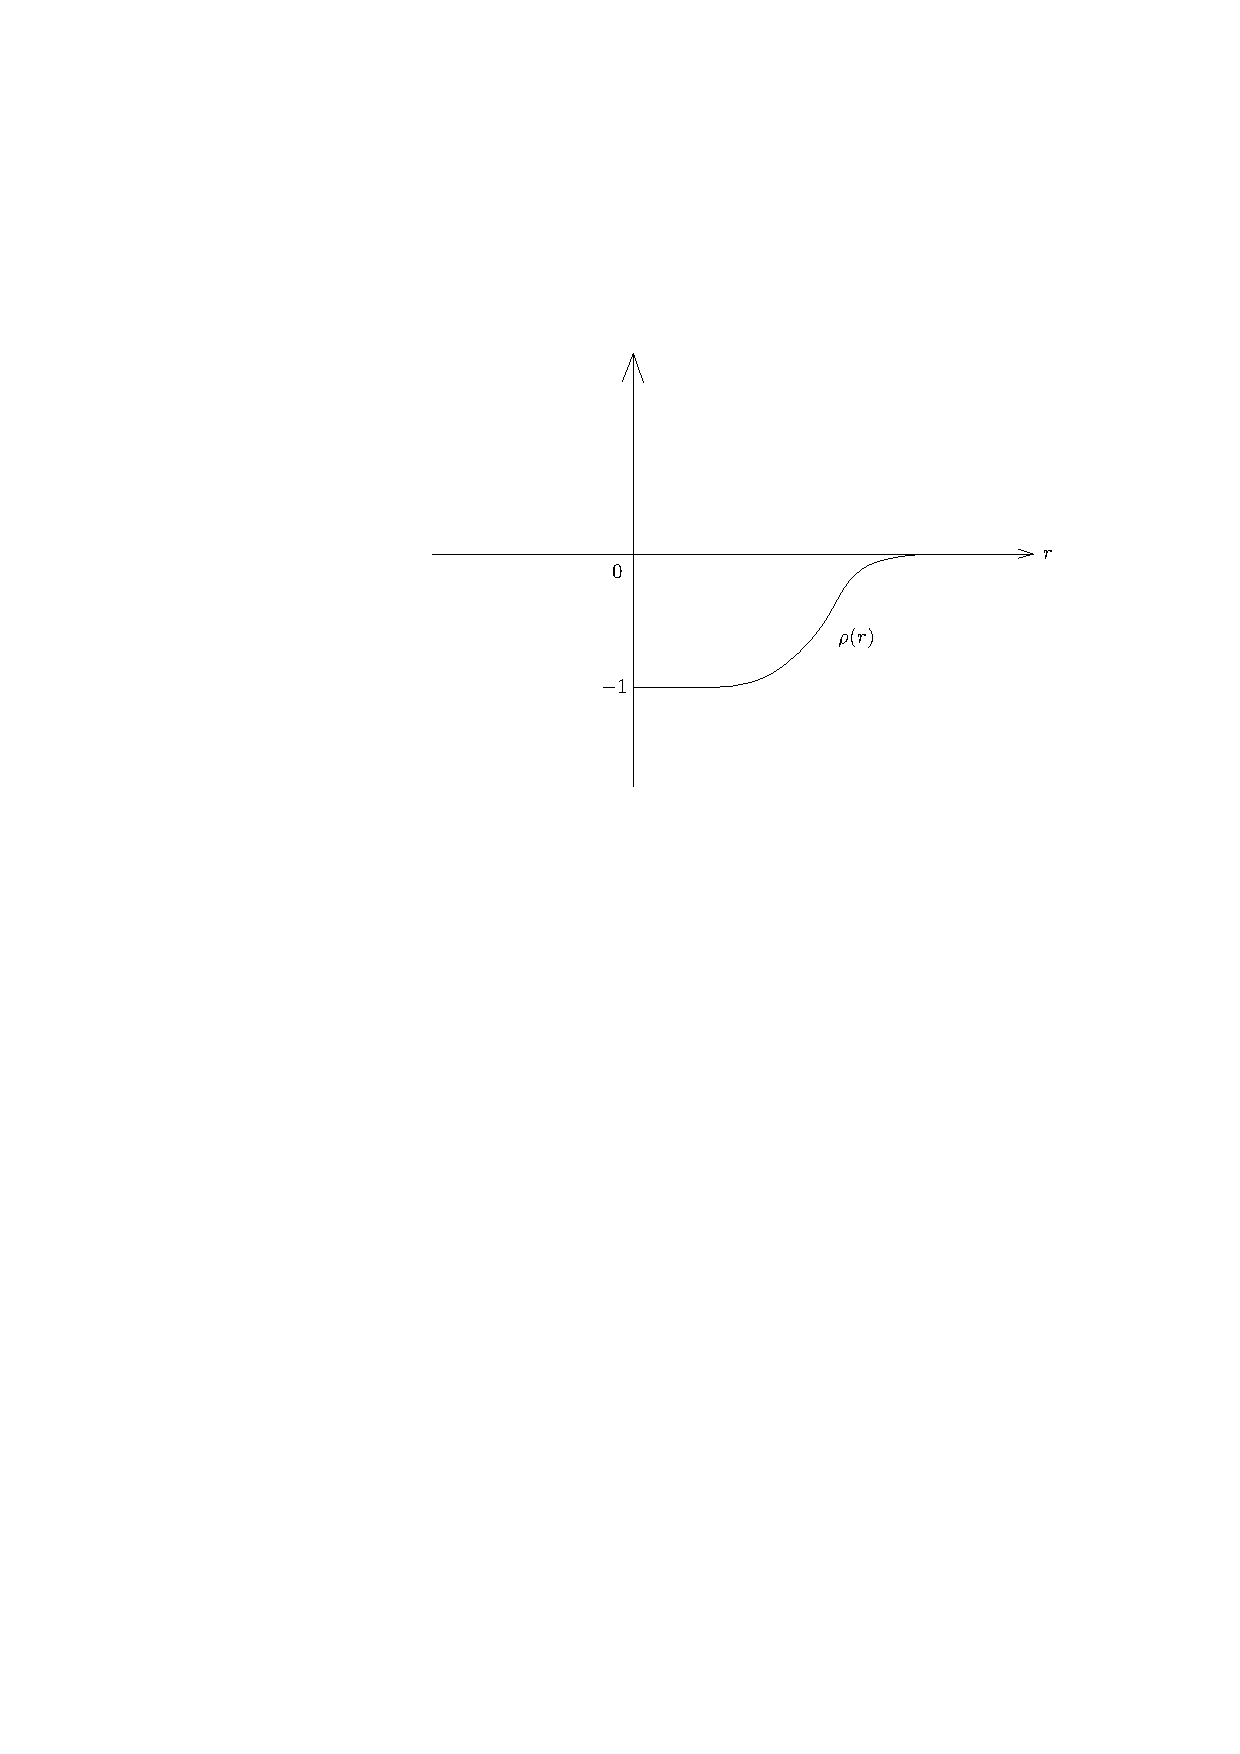
\includegraphics[width=0.5\textwidth]{pictures/Thom-iso-function}
\caption{The function $\rho(r)$.}
\label{Thom iso function rho(r)}
\end{figure}

Let $f:E^0\to S(E)$ be a deformation retraction of the complement of the zero section in $E$ onto the unit sphere bundle. If $\psi_S$ is the global angular form on $S(E)$, 
then $\psi=f^*\psi_S\in H^{k-1}(E^0)$ is the global angular form on $E^0$. It has the property that
\[d\psi=-\pi^*e.\]
where $e$ represents the Euler class of the bundle $E$.
\begin{proposition}
The cohomology class of
\[\Phi=d(\rho(r)\wedge\psi)\in\Omega^k_{cv}(E)\]
is the Thom class of the oriented vector bundle $E$.
\end{proposition}
\begin{proof}
Note that
\[\Phi=d\rho(r)\wedge\psi+\rho(r)\wedge d\psi=d\rho(r)\wedge\psi-\rho(r)\wedge\pi^*e.\]
By our choice of $\rho(r)$, it is easy to see $\Phi\in\Omega_{cv}(E)$ and it is closed. Its restriction to the fiber at $p$ is 
\[\iota_p^*(d(\rho(r)\wedge\psi))=d(\iota_p^*\rho(r)\wedge\iota_p^*\psi)=(d\rho(r))\wedge\iota_p^*\psi-\rho(r)\wedge\iota_p^*\pi^*e,\]
where $i_p:E_p\to E$ is the inclusion and $\iota_p^*$ gives a generator of $H^{k-1}(\R^k\setminus\{0\})=H^{k-1}(S^{k-1})$. From the diagram
\[\begin{tikzcd}
E_p\ar[r]\ar[d]&\{p\}\ar[d]\\
E\ar[r,"\pi"]&M
\end{tikzcd}\]
we see that $\iota_p^*\pi^*e=0$, therefore
\[\int_{\R^k}\iota_p^*\Phi=\int_{\R^k}(d\rho(r))\wedge\iota_p^*\psi=\int_{\R}d\rho(r)\int_{S^{k-1}}\iota_p^*\psi=1.\]
Thus by \cref{Thom iso} $\Phi$ is the Thom class of $E$.
\end{proof}
We now have our promised fact about the Thom class and the Euler class.
\begin{proposition}\label{Thom class pullback Euler class}
The pullback of the Thom class of an oriented rank $k$ vector undle via the zero section to the base manifold is the Euler class.
\end{proposition}
\begin{proof}
Let $s$ be the zero section of $E$. Use the formula of $\Phi$, we find that
\[s^*\Phi=s^*d(\rho(r)\wedge\psi)=s^*((d\rho(r))\wedge\psi-\rho(r)\pi^*e)=s^*d\rho(r)\wedge s^*\psi-s^*\rho(r)s^*\pi^*e=e.\]
Thus we get the claim.
\end{proof}
\begin{remark}
From the formula for the Thom class, it is clear that by making the support of $\rho(r)$ sufficiently close to $0$, the Thom class $\Phi$ can be made to have support 
arbitrarily close to the zero section of the vector bundle.
\end{remark}
\begin{remark}
In fact, any section will pull the Thom class back to the Euler class. Let $s$ be a section of the oriented vector bundle $E$ and $s^*:H_{cv}^*(E)\to H^*(M)$ the 
induced map in cohomology. Note that $s^*$ can be written as the composition of the natural maps $i:H^*_{cv}(E)\to H^*(E)$ and $\widebar{s}^*:H^*(E)\to H^*(M)$. 
As a map from $M$ into $E$, the section $s$ is homotopic to the zero section $s_0$. By the homotopy axiom for de Rham cohomology $\widebar{s}^*=\widebar{s}_0^*$. Hence, 
$s^*=s_0^*$.
\end{remark}
Using the description of the Euler class as the pullback of the Thom class, it is easy to prove the Whitney product formula.
\begin{proposition}[\textbf{Whitney Product Formula for the Euler Class}]
If $E$ and $F$ are two oriented vector bundles, then $e(E\oplus F)=e(E)\wedge e(F)$.
\end{proposition}
\begin{proof}
By \cref{Thom class disrect sum}, the Thorn class of $E\oplus F$ is
\[\Phi(E\oplus F)=\pi_1^*\Phi(E)\wedge\pi_2^*\Phi(F).\]
Let $s$ be the zero section of $E\oplus F$. Then $\pi_1\circ s$ sand $\pi_2\circ s$ are the zero sections of $E$ and $F$. By \cref{Thom class pullback Euler class},
\[e(E\oplus F)=s^*\Phi(E\oplus F)=s^*\pi_1^*\Phi(E)\wedge s^*\pi_2^*\Phi(F)=e(E)\wedge e(F).\]
\end{proof}
\paragraph{Euler class and the zero locus of a section}
Let $\pi:E\to M$ be a vector bundle and $S_0$ the image of the zero section in $E$. A section $s$ of $E$ is \textbf{transversal} if its image $S=s(M)$ intersects $S_0$ 
transversally.
\begin{proposition}\label{tran section normal bundle zero locus}
Let $\pi:E\to M$ be any vector bundle and $Z$ the zero locus of a transversal section. Then $Z$ is a submanifold of $M$ and its normal bundle in $M$ is $NZ=E|_Z$.
\end{proposition}
\begin{proof}
Write $S=s(M)$ for the image of the section $s$. Because $S$ intersects $S_0$ transversally, $S\cap S_0$ is a submanifold of $S$ by the transversality theorem. Under 
the diffeomorphism $s:M\to S$, $Z$ is mapped homeomorphically to $S\cap S_0$. So $Z$ can be made into a submanifold of $M$.\par
To compute the normal bundle of $Z$, we first note that because $E$ is locally trivial, its tangent bundle on $S_0$ has the following canonical decomposition
\[TE|_{S_0}=E|_{S_0}\oplus TS_0.\]
By the transversality of $S\cap S_0$,
\[TS+TS_0=TE=E\oplus TS_0.\]
Therefore we obtain
\[E=\frac{E\oplus TS_0}{TS_0}\cong\frac{TS+TS_0}{TS_0}\cong\frac{TS}{TS\cap TS_0}.\]
This then gives an exact sequence
\[\begin{tikzcd}
0\ar[r]&(TS\cap TS_0)|_Z\ar[r]&TS|_Z\ar[r]&E|_Z\ar[r]&0
\end{tikzcd}\]
Since $(TS\cap TS_0)|_Z=TZ$, we find that $NZ\cong E|_Z$.
\end{proof}
In the proposition above, if $E$ and $M$ are both oriented, then the zero locus $Z$ of a transversal section is naturally an oriented manifold, oriented in such a way 
that
\[E|_Z\oplus TZ=TM|_Z.\]
has the direct sum orientation.
\begin{proposition}
Let $\pi:E\to M$ be an oriented vector bundle over an oriented manifold $M$. Then the Euler class $e(E)$ is Poincar\'e dual to the zero locus of a transversal section.
\end{proposition}
\begin{proof}
We will identify $M$ with the image $S_0$ of the zero section. If $S$ is the image in $E$ of the transversal section $s:M\to E$, then the zero locus of $s$ is $Z=S\cap S_0$. 
$Z$ is a closed oriented submanifold of $M$ and by \cref{tran section normal bundle zero locus}, its normal bundle in $M$ is $NZ\cong E|_Z$. Since $S$ is 
diffeomorphic to $M$, the normal bundle of $Z$ in $S$ is also isomorphic to $E|_Z$. The normal bundles of $Z$ in $M$ and $S$, denoted by $N_MZ$ and $N_SZ$, will be 
identified with the tubular neighborhoods of $Z$ in $M$ and in $S$, respectively.\par
Choose the Thom class $\Phi$ of $E$ to have support so close to the zero section that $\Phi$ restricted to the tubular neighborhood $N_SZ$ in $S$ has compact support 
in the vertical direction. We will now show that $s^*\Phi$ is the Thom class of the tubular neighborhood $N_MZ$ in $M$.\par
Let $E_p$, $S_p$, and $M_p$ be the fibers of $E|_Z$, $N_SZ$, $N_MZ$ respectively above the point $p$ in $Z$. Because $\Phi$ has compact support in $S_p$, $s^*\Phi$ 
has compact support in $M_p$. Furthermore, after identifying $S_p$ and $M_p$ with their conterpart in the tubular neighborhoods, we have the following diffeomorphisms:
\[\begin{tikzcd}
M_p\ar[rd,swap,"\beta"]\ar[r,"s"]&S_p\ar[d,"\alpha"]\\
&E_p
\end{tikzcd}\]
Therefore we get
\begin{align*}
\int_{M_p}s^*\Phi=\int_{M_p}s^*\alpha^*\Phi=\int_{S_p}\alpha^*\Phi=\int_{E_p}\Phi=1.
\end{align*}
So $s^*\Phi$ is the Thom class of $N_MZ$. By \cref{Thom class pullback Euler class}, $s^*\Phi=e(E)$. Since by \cref{Thom class Poincare dual} the 
Thom class of $N_MZ$ is Poincare dual to $Z$ in $M$, the Euler class $e(E)$ is Poincare dual to $Z$ in $M$.
\end{proof}
\paragraph{Poincar\'e duality}
Let $M$ be a manifold of dimension $n$ and $\mathcal{U}=\{U_i\}$ any open cover of $M$. Define the coboundary operator
\[\delta:\bigoplus\Omega^*_c(U_{i_0\dots i_p})\to\bigoplus\Omega^*_c(U_{i_0\dots i_{p-1}})\]
by the formula
\[(\delta\omega)_{i_0\dots i_{p-1}}=\sum_{i}\omega_{i,i_0\dots i_{p-1}}.\]
where on the right-hand side we mean the extension by zero of $\omega_{i,i_0\dots i_{p-1}}$ to a form on $U_{i_0\dots i_{p-1}}$. To ensure that each component of $\delta\omega$ 
has compact support, the groups here are direct sums rather than direct products, so that $\omega$ by definition has only a finite number of nonzero components.
\begin{proposition}[\textbf{Generalized Mayer-Vietoris Sequence for Compact Supports}]\label{Generalized MV compact supp}
Suppose the open cover $\mathcal{U}$ of the manifold $M$ is locally finite. Then the sequence
\[\begin{tikzcd}
\cdots\ar[r]&\bigoplus\Omega^*_c(U_{i_0i_1})\ar[r]&\bigoplus\Omega^*_c(U_{i_0})\ar[r,"\text{sum}"]&\Omega^*_c(M)\ar[r]&0
\end{tikzcd}\]
is exact.
\end{proposition}
\begin{proof}
We first show $\delta^2=0$. Let $\omega$ be in $\bigoplus\Omega^*_c(U_{i_0\dots i_p})$. Then
\[(\delta^2\omega)_{i_0\dots i_{p-2}}=\sum_i(\delta\omega)_{i,i_0\dots i_{p-2}}=\sum_i\sum_j\omega_{j,i,i_0\dots i_{p-2}}=0.\]
(Here we use the alternating condition $\omega_{i_0\dots i\dots j\dots i_p}=-\omega_{i_0\dots j\dots i\dots i_p}$.) Now we define a homotopy from the identity to zero. 
Let $\{\rho_i\}$ be a partition of unity subordinate to the cover $\{U_i\}$. Define a map
\[K:\Omega^*_c(U_{i_0\dots i_p})\to\Omega^*_c(U_{i_0\dots i_{p+1}})\]
by the formula
\[(K\omega)_{i_0\dots i_{p+1}}=\sum_{j=0}^{p+1}(-1)^i\rho_{i_j}\omega_{i_0\dots\widehat{i_j}\dots i_{p+1}}.\]
Note that $(K\omega)_{i_0\dots i_{p+1}}$ has compact support. Moreover, there are only finitely many $(j,i_0,\dots,i_p)$ for which $\rho_j\omega_{i_0\dots i_p}\neq 0$, 
since $\omega_{i_0\dots i_p}\neq 0$ for finitely many $(i_0,\dots,i_p)$ and by the locally finiteness each $U_{i_0\dots i_p}\sub U_{i_0}$ intersects only finitely many 
$U_j$. With this definition, we have
\begin{align*}
(\delta K\omega)_{i_0\dots i_p}&=\sum_i(K\omega)_{i,i_0\dots i_{p}}=\sum_i\rho_{i}\omega_{i_0\dots i_{p}}+\sum_i\sum_{j=0}^{p}(-1)^{j+1}\rho_{i_j}\omega_{i,i_0\dots\widehat{i_{j}}\dots i_{p}}\\
&=\omega_{i_0\dots i_p}-\sum_{j=0}^{p}(-1)^j\rho_{i_j}\sum_i\omega_{i,i_0\dots\widehat{i_{j}}\dots i_{p}}\\
&=\omega_{i_0\dots i_p}-\sum_{j=0}^{p}(-1)^j\rho_{i_j}\sum_i\omega_{i,i_0\dots\widehat{i_{j}}\dots i_{p}}\\
&=\omega_{i_0\dots i_p}-\sum_{j=0}^{p}(-1)^j\rho_{i_j}(\delta\omega)_{i_0\dots\widehat{i_{j}}\dots i_{p}}\\
&=\omega_{i_0\dots i_p}-(K\delta\omega)_{i_0\dots i_p}.
\end{align*}
Therefore $\delta K+K\delta=\id$ and we conclude the claim.
\end{proof}
Consider the double complex $C^*(\mathcal{U},\Omega^*_c)$, where $\mathcal{U}$ is a locally finite cover. In this double complex the $\delta$-operator goes in the wrong 
direction, so we define a new complex
\[K^{-p,q}=C^p(\mathcal{U},\Omega^q_c).\]
Then by \cref{Generalized MV compact supp} and a spectral sequence argument, we get
\[H_{TC}^*(K)=H_c^*(M).\]
On the other hand, by definition we have
\[_{v}E_1^{-p,q}=C^p(\mathcal{U},\mathscr{H}_c^q)\]
where $\mathscr{H}_c^q$ is the covariant functor which associates to every open set $U$ the compact cohomology $H^q_c(U)$ and to every inclusion $i$, the extension by 
zero $i_*$; moreover, is $\mathcal{U}$ is a good cover, then
\[\mathscr{H}_c^q(U)=\begin{cases}
\R,&q=n;\\
0,&q\neq n.
\end{cases}\]
Therefore in this case the $_{v}E_1$ page has only one row, and therefore
\[H^*_{TC}(K)={_{v}E_2^{*-n,n}}=H_{n-*}(\mathcal{U},\mathscr{H}^n_c).\]
Here $H(\mathcal{U},\mathscr{H}^n_c)$ is the tech homology of the cover $\mathcal{U}$ with coefficients in the covariant functor $\mathscr{H}_c^{n}$.
\begin{proposition}
Let $M$ be a manifold of dimension $n$ and $\mathcal{U}$ any locally finite good cover of $M$. Here $M$ is not assumed to be orientable. Then
\[H^*_c(M)\cong H_{n-*}(\mathcal{U},\mathscr{H}^n_c),\]
where $\mathscr{H}^n_c$ is the covariant functor $\mathscr{H}^n_c(U)=H^n_c(U)$.
\end{proposition}
\subsection{Monodromy}
\paragraph{When is a locally constant presheaf constant}
In the preceding part we saw that the compact vertical cohomology $H^*_{cv}(E)$ of a vector bundle $E$ may be computed as the cohomology of the base with 
coefficients in the presheaf $\mathscr{H}_{cv}^n$. When the presheaf $\mathscr{H}_{cv}^n$ is the constant presheaf $\R^n$, $H^*_{cv}(E)$ is expressible in terms of the 
de Rham cohomology of the base manifold. In this case the problem of computing $H^*_{cv}(E)$ is greatly simplified. It is therefore important to 
determine the conditions under which a presheaf such as $\mathscr{H}_{cv}$ is constant.\par
We first introduce the notion of a presheaf on a cover. Let $X$ be a topological space and $\mathcal{U}=\{U_\alpha\}$ a cover of $X$. The presheaf $\mathscr{F}$ on 
$\mathcal{U}$ is defined to be a functor $\mathscr{F}$ on the subcategory of $\mathbf{Open}(X)$ consisting of all finite intersections $U_{i_0\dots i_p}$ of open sets in 
$\mathcal{U}$. Equivalently, if $N(\mathcal{U})$ is the nerve of $\mathcal{U}$, the presheaf $\mathscr{F}$ on $\mathcal{U}$ is the assignment of an appropriate group to 
the barycenter of each simplex in $N(\mathcal{U})$; for example, the group attached to the barycenter of the $2$-simplex representing $U\cap V\cap W$ is 
$\mathscr{F}(U\cap V\cap W)$. Each inclusion, say $U\cap V\hookrightarrow U$, becomes an arrow in the picture, $\mathscr{F}(U)\to\mathscr{F}(U\cap V)$, and the 
transitivity of the arrows says that Figure is a commutative diagram.

Two presheaves $\mathscr{F}$ and $\mathscr{G}$ are isomorphic relative to a cover $\mathcal{U}=(U_i)$ if for each $U_{i_0\dots i_p}$ there is an isomorphism
\[h_{i_0\dots i_p}:\mathscr{F}(U_{i_0\dots i_p})\to\mathscr{G}(U_{i_0\dots i_p})\]
compatible with all arrows. In other words, there is a natural equivalence of functors $\mathscr{F}\to\mathscr{G}$ where $\mathscr{F}$ and $\mathscr{G}$ are regarded as \
functors on the subcategory of $\mathbf{Open}(X)$ consisting of all finite intersections of open sets in $\mathcal{U}$. The constant presheaf with group $G$ on a good 
cover $\mathcal{U}$ is defined as usual, it associates to every open set the group of locally constant and hence constant functions: $U_{i_0\dots i_p}\to G$. Thus, for 
a constant presheaf on a cover, all the groups are $G$ and all the arrows are the identity map. We say that a presheaf $\mathscr{F}$ is \textbf{locally constant} 
on a cover $\mathcal{U}$ if all the groups are isomorphic and all the arrows are isomorphisms.\par
Of course, if two presheaves $\mathscr{F}$ and $\mathscr{G}$ are isomorphic on a cover $\mathcal{U}$, then the \v{C}ech cohomology groups $H^*(\mathcal{U},\mathscr{F})$ 
and $H^*(\mathcal{U},\mathscr{G})$ are isomorphic.\par
Let $\mathscr{F}$ be a locally constant presheaf with group $G$ on a cover $\mathcal{U}=(U_i)$. Fix isomorphisms $\phi_i:\mathscr{F}(U_i)\to G$. If $U_i$ and $U_j$ 
intersect, then from the diagram
\[\begin{tikzcd}
\mathscr{F}(U_i)\ar[d,"\phi_i"]\ar[r,"\rho^i_{ij}"]&\mathscr{F}(U_{ij})&\mathscr{F}(U_j)\ar[l,swap,"\rho^j_{ij}"]\ar[d,"\phi_j"]\\
G\ar[rr,dashed]&&G
\end{tikzcd}\]
we obtain an automorphism of $G$, namely $\phi_j\circ(\rho_{ij}^j)^{-1}\circ\rho^i_{ij}\circ\phi_i^{-1}$. Write $\rho^i_j:\mathscr{F}(U_i)\to\mathscr{F}(U_j)$ for the 
isomorphism $(\rho_{ij}^j)^{-1}\circ\rho^i_{ij}$. Choose some vertex $U_0$ as the base point of the nerve $N(\mathcal{U})$. For $U_0U_1\cdots U_rU_0$ a loop based at 
$U_0$ we get an automorphism of $G$ by following along the edges
\[\begin{tikzcd}
\mathscr{F}(U_0)\ar[d,"\phi_0"]\ar[r]&\mathscr{F}(U_1)\ar[d,"\phi_1"]\ar[r]&\cdots\ar[r]&\mathscr{F}(U_r)\ar[d,"\phi_r"]\ar[r]&\mathscr{F}(U_0)\ar[d,"\phi_0"]\\
G\ar[r]&G\ar[r]&\cdots\ar[r]&G\ar[r]&G
\end{tikzcd}\]
This gives a map from loops at $U_0$ to $\Aut(G)$. By the transitivity of the transition map, we claim that if a loop bounds a $2$-chain in $N(\mathcal{U})$, then the 
associated automorphism of $G$ is the identity. Hence there is a Homomorphism
\[\rho:\pi_1(N(\mathcal{U}))=\frac{\text{loops}}{\text{bounding loops}}\to\Aut(G).\]
called the \textbf{monodromy representation} of the presheaf $\mathscr{F}$. Here $\pi_1(N(\mathcal{U}))$ denotes the edge path group of the simplicial complex $N(\mathcal{U})$.
\begin{theorem}
Let $\mathcal{U}$ be a cover on a connected topological space $X$ and $N(\mathcal{U})$ its nerve. If $\pi_1(N(\mathcal{U}))=0$, then every locally constant presheaf on 
$\mathcal{U}$ is constant.
\end{theorem}
\begin{proof}
For each open set $U_i$, choose a path from $U_0$ to $U_i$, say $U_0U_{i_1}\cdots U_{i_r}U_i$ and define 
\[\psi_i=\phi_0\circ(\rho^{i_r}_i\circ\cdots\circ\rho^{i_1}_{i_2}\circ\rho^0_{i_1})^{-1}:\mathscr{F}(U_i)\to G.\]
$\psi_i$ is well-defined independent of the chosen path, because $\rho$ is trivial. Now carry out the barycentric subdivision of the nerve $N(\mathcal{U})$ to get a 
new simplictal complex $K$ so that every open set $U_{i_0\dots i_p}$ corresponds to a vertex of $K$. Clearl $\pi_1(K)=\pi_1(N(\mathcal{U}))=0$. By the same procedure as 
in the preceding paragraph we can define isomorphisms $\psi_{i_0\dots i_p}:\mathscr{F}(U_{i_0\dots i_p})\to G$. The maps $\psi_{i_0\dots i_p}$ give an isomorphism of 
the presheaf $\mathscr{F}$ to the constant presheaf $G$ on the cover $\mathcal{U}$.
\end{proof}
By a good cover on a topological space we shall mean an open cover for which all finite intersections are contractible.
\begin{theorem}
Suppose the topological space $X$ has a good cover $\mathcal{U}$. Then the fundamental group of $X$ is isomorphic to the fundamental group $\pi_1(N(\mathcal{U}))$ of the 
nerve of the good cover.
\end{theorem}
\begin{corollary}
Let $\mathcal{U}$ be a good cover on a simply connected topological space $X$. Then any locally constant sheaf on $\mathcal{U}$ is constant.
\end{corollary}
\begin{corollary}
Any locally constant sheaf on a simply connected manifold is constant.
\end{corollary}
\subsection{The spectral sequence of a fiber bundle}
Let $\pi:E\to M$ be a fiber bundle with fiber $F$ over a manifold $M$. Applying spectral sequence gives a general method for computing the cohomology of $E$ from that 
of $F$ and $M$. Indeed, given a good cover $\mathcal{U}$ of $M$, $\pi^{-1}(\mathcal{U})$ is a cover on $E$ and we can form the double complex 
$C^*(\pi^{-1}(\mathcal{U}),\Omega^*)$, whose $E_1$ term is
\[E_1^{p,q}=\prod H^q(\pi^{-1}(U_{i_0\dots i_p}))=C^p(\pi^{-1}(\mathcal{U}),\mathscr{H}^q).\]
where $\mathscr{H}^q$ is the presheaf $\mathscr{H}^q(U)=H^q(\pi^{-1}(U))$ on $M$. For emphasis we sometimes write the presheaf $\mathscr{H}^q$ as $\mathscr{H}^q(F)$. 
Since $\mathcal{U}$ is a good cover, $E|_{U_i}$ is trivial and thus $\mathscr{H}^q$ is a locally constant presheaf on $\mathcal{U}$ with group $H^q(F)$. Since $d_1=\delta$ 
on $E_1$, the $E_2$ term is
\[E_2^{p,q}=H^p(\mathcal{U},\mathscr{H}^q).\]
By the generalized Mayer-Vietoris principle $H^*_{TC}(C^*(\pi^{-1}(\mathcal{U}),\Omega^*))$ is equal to $H^*(E)$, because $\pi^{-1}(\mathcal{U})$ is a cover on $E$. 
In the case that $\mathscr{H}^q$ is constant and $H^q(F)$ is finite-dimensional, the $E_2$ term is isomorphic as a vector space to the tensor product $H^p(M)\otimes H^q(F)$, 
since
\[E_2^{p,q}=H^p(\mathcal{U},\R^{\dim H^q(F)})=H^p(\mathcal{U},\R)\otimes H^q(F)=H^p(M)\otimes H^q(F).\]
Therefore we have proved the following.
\begin{proposition}[\textbf{Leray's Theorem for de Rham Cohomology}]
Given a fiber bundle $\pi:E\to M$ with fiber $F$ over a manifold $M$ and a good cover $\mathcal{U}$ of $M$, there is a spectral sequence $\{E_r\}$ converging to the 
cohomology of the total space $H^*(E)$ with
\[E_2^{p,q}=H^p(\mathcal{U},\mathscr{H}^q).\]
where $\mathscr{H}^q$ is the locally constant presheaf $\mathscr{H}^q(U)=H^q(\pi^{-1}(U))$ on $\mathcal{U}$. If $\mathscr{H}^q$ is constant (for example, if $M$ is 
simply connected) and $H^q(F)$ is finite-dimensional, then
\[E_2^{p,q}=H^p(M)\otimes H^q(F).\]
\end{proposition}
\begin{example}[\textbf{The K\"unneth formula and the Leray-Hirsch theorem}]
We now give a spectral sequence proof of the K\"unneth formula. Let $M$ and $F$ be two manifolds and $\mathcal{U}$ a good cover of $M$. Suppose $F$ has 
finite-dimensional cohomology. By Leray's theorem, the spectral sequence of the trivial bundle $F\to M\times F\to M$ has $E_2$ term
\[E_2^{p,q}=H^p(\mathcal{U},\mathscr{H}^q).\]
Because $M\times F$ is a trivial bundle over $M$, the presheaf $\mathscr{H}^q(F)$ is constant, so that
\[E_2^{p,q}=H^p(\mathcal{U},\R)\otimes H^q(F)=H^p(M)\otimes H^q(F).\]
The differential $d_r$ measures the extent to which an element of $C^*(\pi^{-1}(\mathcal{U}),\Omega^*)$ that lives to $E_r$ fails to be extended one step further to a 
$D$-cocycle. Since every element of the $E_2$ term is already a global form on $M\times F$. So $E_2=E_{\infty}$. Therefore we get the K"unneth formula
\[H^*(M\times F)=H^*(M)\otimes H^*(F).\]
The proof of the Leray-Hirsch theorem is analogous.
\end{example}
\begin{example}[\textbf{Orientability and the Euler class of a sphere bundle}]\label{Orientability of sphere bundle spectral seq}
Let $\pi:E\to M$ be an $S^k$-bundle over a manifold $M$ and let $\mathcal{U}$ be a good cover of $M$. The spectral sequence of this fiber bundle has
\[E_1^{p,q}=C^p(\mathcal{U},\mathscr{H}^q(S^k))=\begin{cases}
C^p(\mathcal{U},\R),&q=0,k;\\
0,&\text{otherwise}
\end{cases}.\]
Let $\sigma$ be the element of $E_1^{0,k}$ corresponding to the local angular forms on the sphere bundle $E$. From the description of the differential $d_r$ as the $\delta$ 
of the tail of a zig-zag, we see that $E$ is orientable if and only if $d_1\sigma=0$. For an orientable $S^k$-bundle then, such a $\sigma$ lives to $E_k$:
\[E_k=E_2=H^*(\mathcal{U},\mathscr{H}^*(S^k)).\]
Up to a sign $d_k\sigma$ in $H^{k+1}(\mathcal{U},\mathscr{H}^0(S^k))=H^{k+1}(\mathcal{U},\R)=H^{k+1}(M)$ is the Euler class of the sphere bundle. It measures the extent 
to which $\sigma$ fails to be extended to a $D$-cocycle, i.e., a global closed $k$-form on the sphere bundle.
\end{example}
\begin{example}[\textbf{Orientability of a simply connected manifold}]
Let $M$ be a simply connected manifold of dimension $n$ and $S(TM)$ its unit tangent bundle. The spectral sequence of the fiber bundle
\[\begin{tikzcd}
S^{k-1}\ar[r]&S(TM)\ar[r]&M
\end{tikzcd}\]
has $E_2$ term
\[E_2=H^*(\mathcal{U},\mathscr{H}^*(S^k)).\]
Since each restricted bundle on $U_{i_0\dots i_p}$ is trivial, $\mathscr{H}^0(S^k)$ and $\mathscr{H}^k(S^k)$ is contant on it. Therefore
\[E_2^{p,q}=H^p(\mathcal{U},\mathscr{H}^q(S^{n-1}))=\begin{cases}
H^p(\mathcal{U},\R)&q=0,n-1\\
0&\text{otherwise}
\end{cases}\]
Moreover, by the isomorphism $H^*(M)=H^*(\mathcal{U},\R)$ and the simply connected condition, we further have
\[E_2^{1,0}=E_2^{1,n-1}=0.\]
This, together with \cref{Orientability of sphere bundle spectral seq}, shows that there is an element in $C^0(\pi^{-1}(\mathcal{U}),\mathscr{H}^{n-1})$ which 
can be extended one step down toward being a $D$-cocycle. Therefore $S(TM)$ and also $M$ are orientable. This gives an alternative proof of the orientability of a simply 
connected manifold.
\end{example}
\begin{example}[\textbf{The cohomology of the complex projective space}]\label{cohomology CP^n}
Consider the sphere $S^{2n+1}$ in $\C^{n+1}$. Let $S^1$ act on $S^{2n+1}$ by
\[\lambda\cdot (z_0,\dots,z_n)=(\lambda z_0,\dots,\lambda z_n).\]
where $\lambda$ in $S^1$ is a complex number of absolute value $1$. The quotient of $S^{2n+1}$ by this action is the complex projective space $\CP^n$. This gives $S^{2n+1}$ 
the structure of a circle bundle over $\CP^n$:
\[\begin{tikzcd}
S^1\ar[r]&S^{2n+1}\ar[r]&\CP^n
\end{tikzcd}\]
As we will see from the homotopy exact sequence to be discussed later, $\CP^n$ is simply connected. Thus
\[E_2^{p,q}=H^p(\CP^n)\otimes H^q(S^1).\]
So $E_2$ has only two nonzero rows, $q=0,1$, and the two rows are identical, both being $H^*(\CP^n)$. Because $\CP^n$ has dimension $2n$, we have $H^p(\CP^n)=0$ for 
$p>2n$. In the spectral seuqnece we have $d_r=0$ for $r>2$, therefore $E_3=E_4=\cdots=E_{\infty}=H^*(S^{2n+1})$. Therefore $E_3$ is
\[\begin{tikzcd}[column sep=0.8em,row sep=0.8em]
0&0&0&\cdots&\R\\
\R&0&0&\cdots&0\\
\end{tikzcd}
\]
From this we can chase the maps in $E_2$. Since $E_2^{0,0}=E_2^{0,1}=\R$ and $E_2^{p,0}=E_2^{p,1}$, we finally conclude that $E_2$ has the form
\[\begin{tikzcd}[column sep=0.8em,row sep=0.8em]
\R\ar[rrd]&0&\R\ar[rrd]&0&\cdots&\R\ar[rrd]&0&\R\\
\R&0&\R&0&\cdots&\R&0&\R\\
\end{tikzcd}\]
Further, from this spectral sequence we can get the product structure of $H^*(\CP^n)$:
\[\begin{tikzcd}[column sep=0.8em,row sep=0.8em]
a\ar[rrd]&&ax\ar[rrd]&&ax^2&\cdots&ax^{n-1}\ar[rrd]&&ax^{n}\\
1&&x&&x^2&\cdots&x^{n-1}&&x^{n}
\end{tikzcd}\]
Therefore
\[H^*(\CP^n)=\R[x]/(x^{n+1}),\quad \dim x=2.\]

Note that $S^{2n-1}$ is a circle bundle on $\CP^n$, so we can compute its Euler class. By definition, the Euler class is given by the diagram
\[\begin{tikzcd}
\sigma\ar[r]&{}&\\
&\ar[r,"\delta"]\ar[u]&d_2(\sigma)=-\pi^*\eps
\end{tikzcd}\]
where $\sigma$ is a generator of $E_2^{0,1}$. By our choice of $a$ and $x$, it is clear that $x=-e$, therefore the Euler class of $S^{2n-1}$ generates the cohomology ring of $\CP^n$.
\end{example}
\paragraph{The Gysin sequence}
The spectral sequence of a fiber bundle is essentially a way of describing the complicated algebraic relations among the cohomology of the base space, the fiber, and 
the total space of the bundle, In certain special situations the spectral sequence simplifies to a long exact sequence, One such special case is the cohomology of a 
sphere bundle. The resulting sequence is called the \textbf{Gysin sequence}, which we now derive.
Let $\pi:E\to M$ be an oriented sphere bundle with fiber $S^k$. By the orientability assumption, for any good cover $\mathcal{U}$ on $M$, the locally constant presheaf 
$\mathscr{H}^k$ has no monodromy and is the constant presheaf $\R$. Therefore the $E_2$ term of the spectral sequence only has two nonzero rows:
\[E_2^{p,q}=H^p(M)\otimes H^q(S^k).\]
This then means $E_2=E_3=\cdots=E_{k+1}$, and we get an exact seuqnece:
\begin{equation}\label{Gysin seq-1}
\begin{tikzcd}
0\ar[r]&E_{\infty}^{p-k,k}\ar[r]&E_2^{p-k,k}\ar[r,"d_{k+1}"]&E_2^{p+1,0}\ar[r]&E_{\infty}^{p+1,0}\ar[r]&0\\
&&H^{p-k}(M)\ar[u,equal]&H^{p+1}(M)\ar[u,equal]&&
\end{tikzcd}
\end{equation}
Because of the shape of the $E_2$ term, the filtration on $H^*(E)$ becomes
\[H^p(E)\sups E^{p,0}_{\infty}\sups 0,\quad H^p(E)/E^{p,0}\cong E^{p-k,k}_{\infty}.\]
In other words, there is an exact sequence
\begin{equation}\label{Gysin seq-2}
\begin{tikzcd}
0\ar[r]&E^{p,0}_{\infty}\ar[r]&H^p(E)\ar[r]&E_\infty^{p-k,k}\ar[r]&0
\end{tikzcd}
\end{equation}
The two sequences $(\ref{Gysin seq-1})$ and $(\ref{Gysin seq-2})$ may be combined into a single long exact sequence
\[\begin{tikzcd}
\cdots\ar[r]&H^p(E)\ar[r,"\alpha"]&H^{p-k}(M)\ar[r,"d_{k+1}"]&H^{p+1}(M)\ar[r,"\beta"]&H^{p+1}(E)\ar[r]&\cdots
\end{tikzcd}\]
This is the \textbf{Gysin sequence} of the sphere bundle.\par
It remains to identify the maps in the Gysin sequence. Let $\mathcal{U}$ be a good cover on $M$. The map $\alpha$ is the composition
\[\begin{tikzcd}[column sep=1.2em]
H^p(E)\ar[r]&E_{\infty}^{p-k,k}\ar[r,hook]&E_2^{p-k,k}=H^{p-k}(\pi^{-1}(\mathcal{U}),\mathscr{H}^k)\cong H^{p-k}(M)\otimes H^k(S^k)\cong H^{p-k}(M)
\end{tikzcd}\]
In this sequence of maps the first three are the identity on the level of forms and the last one sends a generator of $H^k(S^k)$ to $1$ by integration. Therefore $\alpha$ 
is integration along the fiber.\par
Next consider $d_{k+1}$. By representing an element of $E_2^{p-k,k}=H^{p-k}(M)\otimes H^k(S^k)$ by $(\pi^*\omega)\wedge(-\psi)$, where $\omega$ is a closed form on $M$ 
and $\psi$ is the global angular form on $E$ (note that $\psi$ is locally closed), the map $d_{k+1}$ is defined to be
\begin{align*}
d_{k+1}(\omega)&:=d_{k+1}((\pi^*\omega)\wedge(-\psi))\\
&=d((\pi^*\omega)\wedge(-\psi))=d(\pi^*\omega)\wedge(-\psi)+(-1)^{p-k}(\pi^*\omega)\wedge d(-\psi)\\
&=(-1)^{pxs-k}\pi^*\omega\wedge\pi^* e=(-1)^{p-k}\pi^*(\omega\wedge e).
\end{align*}
Hence, up to a sign $d_{k+1}:H^{p-k}(M)\to H^{p+1}(M)$ is multiplication by the Euler class $e$.\par
Finally the map $\beta$ is the composition
\[\begin{tikzcd}[column sep=1.2em]
H^{p+1}(M)=H^{p+1}(\mathcal{U},\mathscr{H}^0)\ar[r,"\pi^*"]\ar[r,swap,"\cong"]&H^{p+1}(\pi^{-1}(\mathcal{U}),\mathscr{H}^0)=E_2^{p+1,0}\ar[r]&E_{\infty}^{p+1,0}\ar[r,hook]&H^{p+1}(E)
\end{tikzcd}\]
So $\beta:H^{p+1}(M)\to H^{p+1}(E)$ is the natural pullback map $\pi^*$.\par
We summarize this discussion as follows.
\begin{theorem}
Let $\pi:E\to M$ be an oriented sphere bundle with fiber $S^k$. Then there is a long exact sequence
\[\begin{tikzcd}
\cdots\ar[r]&H^p(E)\ar[r,"\pi_*"]&H^{p-k}(M)\ar[r,"\wedge e"]&H^{p+1}(M)\ar[r,"\pi^*"]&H^{p+1}(E)\ar[r]&\cdots
\end{tikzcd}\]
where $e$ is the Euler class of $E$.
\end{theorem}
\paragraph{Leray's construction}
We consider now more generally not a fiber bundle but any map $f:X\to Y$ from one manifold to another, and study how the cohomology groups of $X$ relate to those of $Y$. 
Let $\mathcal{U}$ be any cover for $Y$, not necessarily a good cover. Then $\pi^{-1}(\mathcal{U})$ is a cover for $X$. By the Mayer-Vietoris principle
\[H^*(X)=H^*_{TC}(C^*(\pi^{-1}(\mathcal{U}),\Omega^*).\]
The spectral sequence of this double complex has
\[E_2^{p,q}=H^p(\mathcal{U},\mathscr{H}^q),\]
where $\mathscr{H}^q$ is the presheaf on $Y$ defined by $\mathscr{H}^q(U)=H^q(f^{-1}(U))$.
The main difference between this situation and that of a fiber bundle is that the presheaf $\mathscr{H}^q$ is no longer locally constant on $U$; indeed the groups 
$H^q(f^{-1}(U))$ will in general be different for different contractible open sets $U$.
\begin{example}
Let $f:X\to Y$ be any smooth map between manifolds and $\mathcal{U}$ a finite good cover of $Y$. Then from the spectral sequence we have
\begin{align*}
\dim H^n(X)&=\sum_{p+q=n}\dim E_{\infty}^{p,q}=\cdots=\sum_{p+q=n}\dim E_{1}^{p,q}=\sum_{p+q=n}\dim C^p(\mathcal{U},\mathscr{H}^q)\\
&=\sum_{p+q=n}\sum_{i_0\dots i_p}\dim H^q(f^{-1}(U_{i_0\dots i_p})).
\end{align*}
This then implies
\[\chi(X)=\sum_n(-1)^n\sum_{p+q=n}\sum_{i_0\dots i_p}\dim H^q(f^{-1}(U_{i_0\dots i_p})).\]
If in particular $\pi:X\to Y$ is a fiber bundle with fiber $F$, $Y$ admits a finite good cover and $F$ has finite-dimensional cohomology, then
\begin{align*}
\chi(X)&=\sum_n(-1)^n\sum_{p+q=n}\sum_{i_0\dots i_p}\dim H^q(\pi^{-1}(U_{i_0\dots i_p}))\\
&=\sum_n(-1)^n\sum_{p+q=n}\sum_{U_{i_0\dots i_p}\neq\emp}\dim H^q\\
&=\sum_{p+q=n}(-1)^n\dim C^p(\mathcal{U},Y)\cdot \dim H^q(F)\\
&=\chi(Y)\chi(F).
\end{align*}
\end{example}
\subsection{Spectral sequence for singular cohomology}
\paragraph{The Mayer-Vietoris sequence for singular chains}
Let $U=\{U_i\}$ be an open cover of the topological space $X$. Just as for differential forms on a manifold, the sequence of inclusions
\[\begin{tikzcd}
X&\coprod_iU_i\ar[l]&\coprod_{i,j}U_{ij}\ar[l]&\cdots\ar[l]
\end{tikzcd}\]
induces a Mayer-Vietoris sequence. However, we must consider here the group $C^{\mathcal{U}}(X)$ of $\mathcal{U}$-small chains in $X$; these are chains made up of 
simplices each of which lies in some open set of the cover $\mathcal{U}$. The inclusion
\[i:C^{\mathcal{U}}_*(X)\to C_*(X)\]
is a homotopy equivalence, hence induces an isomorphism on homology groups.\par
Now we define a boundary operator
\[\delta:\bigoplus C_q(U_{i_0\dots i_p})\to \bigoplus C_q(U_{i_0\dots i_{p-1}})\]
by the alternating sum formula
\[(\delta c)_{i_0\dots i_p}=\sum_ic_{i,i_0\dots i_{p-1}}.\]
Here, as always, we adopt the alternating convention for chains. The fact that $\delta^2=0$ is proved as in \cref{Generalized MV compact supp}. The boundary 
operator $\delta$ on $\bigoplus C_q(U_i)\to C_q(X)$ is simply the sum; we denote this by $\eps$.
\begin{proposition}
The following sequence is exact
\[\begin{tikzcd}
0&C_*^{\mathcal{U}}\ar[l]&\bigoplus C_*(U_i)\ar[l]&\bigoplus C_*(U_{ij})\ar[l]&\cdots\ar[l]
\end{tikzcd}\]
\end{proposition}
Applying the functor $\Hom(-,\Z)$ to the Mayer-Vietoris sequence for singular chains we obtain the Mayer-Vietoris sequence for singular cochains
\[\begin{tikzcd}
0\ar[r]&C^*_{\mathcal{U}}(X)\ar[r]&\prod C^*(U_i)\ar[r]&\prod C^*(U_{i_0 i_1})\ar[r]&\cdots
\end{tikzcd}\]
Since the functor $\Hom(-,\Z)$ preserves the exactness of a sequence of free $\Z$-modules, the Mayer-Vietoris sequence for singular cochains is exact.\par
Once we have the Mayer-Vietoris sequence we can set up the double complex $C^*(\mathcal{U},C^*)$. Just as in the de Rham theory the double complex computes the singular 
cohomology of $X$:
\[H^*_{TC}(C^*(\mathcal{U},C^*))=H^*(X).\]
If $\mathcal{U}$ is a good cover of a topological space $X$, then by the same argument as in the \v{C}ech-de Rham case, we get
\[H^*_{TC}(C^*(\mathcal{U},C^*))=H^*(\mathcal{U},\Z).\]
Suppose $X$ triangularizable. Since the good covers are cofinal in the set of all covers of $X$, we have
\[H^*(X,\Z)=H^*(\mathcal{U},\Z),\]
where $H^*(X,\Z)$ is the \v{C}ech cohomology of $X$ with coefficients in the constant presheaf $\Z$. Therefore,
\begin{theorem}
The singular cohomology of a triangularizable space $X$ is isomorphic to its \v{C}ech cohomology with coefficients in the constant presheaf $\Z$. If $\mathcal{U}$ is a 
good cover of $X$, then
\[H^*(X)\cong H^*(X,\Z)\cong H*(\mathcal{U},\Z).\]
\end{theorem}
Let $\pi:E\to X$ be a fiber bundle with fiber $F$ over a triangularizable topological space $X$. Just as in Theorem 14.18, from the double complex $C^*(\pi^{-1}(\mathcal{U}),C^*)$ 
on $E$ we obtain a spectral sequence converging to the singular cohomology $H^*(E)$ whose $E_2$ term is
\[E_2^{p,q}=H^p(\mathcal{U},\mathscr{H}^q(F)).\]
If $\mathscr{H}^q(F)$ happens to be the constant presheaf $\Z^n$ on $\mathcal{U}$, then
\[E_2^{p,q}=H^p(\mathcal{U},\Z^n)=H^p(X)\otimes H^q(F).\]

By a similar arguments there is also a Mayer-Vietoris sequence for singular cochains with coefficients in a commutative ring $R$. Using the cup product in place of the 
wedge product, the spectral sequence of the Cech-singular complex $C^*(\mathcal{U},C^*)$ can be given a product structure. The arguments before carry over mutatis 
mutandis. Hence the results on spectral sequences remain true for singular cohomology with coefficients in $R$. However, note that the $E_2$ term of a fiber bundle 
$\pi:E\to X$ with fiber $F$ over a simply connected base space $M$ is the tensor product $H^*(X;\R)\otimes H^*(F;R)$ only if the cohomology of $F$ is a free $R$-module. 
In summary we have the following.
\begin{theorem}[\textbf{Leray's Theorem for Singular Cohomology with Coefficients $\bm{R}$}]
Let $\pi:E\to X$ be a fiber bundle with fiber $F$ over a topological space $X$ and $\mathcal{U}$ an open cover of $X$. Then there is a spectral sequence converging to 
$H^*(E;R)$ with $E_2$ term
\[E_2^{p,q}=H^p(\mathcal{U},\mathscr{H}^q(F;R)).\]
Each $E_r$ in the spectral sequence can be given a product structure relative to which the differential $d_r$ is an antiderivation. If $X$ is simply connected and has
a good cover, then
\[E_2^{p,q}=H^p(X,H^q(F;R)).\]
Ifin addition $H^*(F;R)$ is a finitely generated free $R$-module, then
\[E_2=H^*(X;R)\otimes H^*(F;R)\]
as $R$-algebras.
\end{theorem}
\section{Characteristic classes}
\subsection{Chern classes of a complex vector bundle}
In this part we will study the characteristic classes of a complex vector bundle. To begin with we define the first Chern class of a complex line bundle as the Euler 
class of its underlying real bundle. Applying the Leray-Hirsch theorem, we then compute the cohomology ring of the projectivization $P(E)$ of a complex vector bundle $E$ 
and define the Chern classes of $E$ in terms of the ring structure of $H^*(P(E))$. We conclude with a list of the main properties of the Chern classes.
\paragraph{The first Chern class of a complex line bundle}
Recall that a complex vector bundle of rank $n$ is a fiber bundle with fiber $\C^n$ and structure group $\GL(n,\C)$. A complex vector bundle of rank $1$ is also called 
a complex line bundle. Just as the structure group of a real vector bundle can be reduced to the orthogonal group $\O(n)$, by the Hermitian analogue the structure group 
of a rank $n$ complex vector bundle can be reduced to the unitary group $\U(n)$. Every complex vector bundle $E$ of rank $n$ has an underlying real vector bundle $E_\R$ 
of rank $2n$, obtained by discarding the complex structure on each fiber. By the isomorphism of $\U(1)$ with $\SO(2)$, this sets up a one-to-one correspondence between 
the complex line bundles and the oriented rank $2$ real bundles. We define the first Chern class of a complex line bundle $L$ over a manifold $M$ to be the Euler class 
of its underlying real bundle $L_{\R}$: $c_1(L)=e(L_{\R})\in H^2(M)$.\par
If $L$and $L'$ are complex line bundles with transition functions $\{\tau_{\alpha\beta}\}$ and $\{\tau'_{\alpha\beta}\}$,
\[\tau_{\alpha\beta},\tau'_{\alpha\beta}:U_\alpha\cap U_\beta\to\C^*.\]
then their tensor product $L\otimes L'$ is the complex line bundle with transition functions $\{\tau_{\alpha\beta}\cdot\tau'_{\alpha\beta}\}$. By the formula 
$(\ref{Euler class rank 2 transition})$ which gives the Euler class in terms of the transition functions, we have
\begin{align}\label{Chern first tensor prod}
c_1(L\otimes L')=c_1(L)+c_1(L').
\end{align}

Let $L^*$ be the dual of $L$. Since the line bundle $L\otimes L^*=\Hom(L,L)$ has a nowhere vanishing section given by the identity map, $L\otimes L^*$ is a trivial 
bundle. By $(\ref{Chern first tensor prod})$, $c_1(L)+c_1(L^*)=c_1(L\otimes L^*)=0$. Therefore, $c_1(L^*)=-c_1(L)$.
\begin{example}[\textbf{Tautological bundles on a projective space}]
Let $V$ be a complex vector space of dimension $n$ and $\mathbb{P}(V)$ its projectivization:
\[\mathbb{P}(V)=\{\text{$1$-dimensional subspaces of $V$}\}.\]
On $\mathbb{P}(V)$ there are several God-given vector bundles: the product bundle $\widehat{V}=\mathbb{P}(V)\times V$, the universal subbundle $S$, which is the 
subbundle of $V$ defined by
\[S=\{(\ell,v)\in\mathbb{P}(V)\times V:v\in\ell\}.\]
and the \textbf{universal quotient bundle} $Q$, defined by the exact sequence
\[\begin{tikzcd}
0\ar[r]&S\ar[r]&\widehat{V}\ar[r]&Q\ar[r]&0
\end{tikzcd}\]
The fiber of $S$ above each point $\ell$ in $\mathbb{P}(V)$ consists of all the points in $\ell$, where $\ell$ is viewed as a line in the vector space $V$. The sequence above 
is called the \textbf{tautological exact sequence} over $\mathbb{P}(V)$, and $S^*$ the \textbf{hyperplane bundle}.\par
We now compute the cohomology of $\mathbb{P}(V)$. Endow $V$ with a Hermitian metric and let $E$ be the unit sphere bundle of the universal subbundle $S$:
\[E=\{(\ell,v):v\in\ell,\|v\|=1\}.\]
Since the complement of the zero section $S^0$ is diffeomorphic to $V\setminus\{0\}$, we see the map $\pi:E\to\mathbb{P}(V)$ gives a fibering
\[S^1\to S^{2n-1}\to \mathbb{P}(V).\]
By a computation similar to \cref{cohomology CP^n}, the cohomology ring $H^*(\mathbb{P}(V))$ is seen to be generated by the Euler class of the circle bundle $E$, i.e., the first Chern class 
of the universal subbundle $S$. It is customary to take $x=c_1(S^*)=-c_1(S)$ to be the generator and write
\[H^*(\mathbb{P}(V))=\R[x]/(x^n),\quad n=\dim_\C V.\]
We then see that the Poincar\'e series of the projective space $\mathbb{P}(V)$ is
\[P_t(\mathbb{P}(V))=1+t^2+\cdots+t^{2(n-1)}=\frac{1-t^{2n}}{1-t^2}.\]
\end{example}
\paragraph{The projectivization of a vector bundle}
Let $\rho:E\to M$ be a complex vector bundle with transition functions $\tau_{\alpha\beta}:U_\alpha\cap U_\beta\to\GL(n,\C)$. We write $E_p$ for the fiber over $p$ and 
$\PGL(n,\C)$ for the projective general linear group $\GL(n,\C)/\{\text{scalar matrices}\}$. The projectivization of $E$, $\pi:\mathbb{P}(E)\to M$, is by definition the 
fiber bundle whose fiber at a point $p$ in $M$ is the projective space $\mathbb{P}(E_p)$ and whose transition functions 
$\tau_{\alpha\beta}:U_{\alpha}\cap U_\beta\to\PGL(n,\C)$ are induced from $\tau_{\alpha\beta}$. Thus a point of $\mathbb{P}(E)$ is a line $\ell_p$ in the fiber $E_p$.\par
As on the projectivization of a vector space, on $\mathbb{P}(E)$ there are several tautological bundles: the pullback $\pi^*E$, the universal subbundle $S$, and the 
universal quotient bundle $Q$.
\[\begin{tikzcd}[column sep=0.8em]
0\ar[r]&S\ar[r]&\pi^*E\ar[d]\ar[r]&Q\ar[r]&0&&&E\ar[d,"\rho"]\\
&&\mathbb{P}(E)\ar[rrrrr,"\pi"]&&&&&M
\end{tikzcd}\]
The pullback bundle $\pi^*E$ is the vector bundle over $\mathbb{P}(E)$ whose fiber at $\ell_p$ is $E_p$. When restricted to the fiber $\pi^{-1}(p)$ it becomes the 
trivial bundle,
\[\pi^*E|_{\pi^{-1}(p)}=\mathbb{P}(E)_p\times E_p.\]
since $\rho:E_p\to\{p\}$ is a trivial bundle. The universal subbundle $S$ over $\mathbb{P}(E)$ is defined by
\[S=\{(\ell_p,v)\in\pi^*E:v\in\ell_p\}.\]
Its fiber at $\ell_p$ consists of all the points in $\ell_p$. The universal quotient bundle $Q$ is determined by the tautological exact sequence
\[\begin{tikzcd}
0\ar[r]&S\ar[r]&\pi^*E\ar[r]&Q\ar[r]&0
\end{tikzcd}\]
Set $x=c_1(S^*)$, then $x$ is a cohomology class in $H^2(\mathbb{P}(E))$. Since the restriction of the universal subbundle $S$ on $\mathbb{P}(E)$ to a fiber 
$\mathbb{P}(E_p)$ is the universal subbundle $S$ of the projective space $\mathbb{P}(E)$, by the naturality property of the first Chern class, it follows that $c_1(S)$ 
is the restriction of $-x$ to $\mathbb{P}(E_p)$. Hence the cohomology classes $1,x,\dots,x^{n-1}$ are global classes on $\mathbb{P}(E)$ whose restrictions to each fiber 
$\mathbb{P}(E_p)$ freely generate the cohomology of the fiber. By the Leray-Hirsch theorem the cohomology $H^*(\mathbb{P}(E))$ is a free module over $H^*(M)$ with basis 
$\{1,x,\dots,x^{n-1}\}$. So $x^n$ can be written uniquely as a linear combination of $1,x,\dots,x^{n-1}$ with coefficients in $H^*(M)$; these coefficients are by 
definition the \textbf{Chern classes} of the complex vector bundle $E$:
\begin{align}\label{Chern class def}
x^n+c_1(E)x^{n-1}+\dots+c_n(E)=0,\quad c_i(E)\in H^{2i}(M).
\end{align}
In this equation by $c_i(E)$ we really mean $\pi^*c_i(E)$. We call $c_i(E)$ the $i$-th Chern class of $E$ and
\[c(E)=1+c_1(E)+\dots+c_n(E)\in H^*(M)\]
its \textbf{total Chern class}. With this definition of the Chern classes, we see that the ring structure of the cohomology of $\mathbb{P}(E)$ is given by
\[H^*(\mathbb{P}(E))=H^*(M)[x]/(x^n+c_1(E)x^{n-1}+\dots c_n(E)),\]
where $x=c_1(S^*)$ and $n$ is the rank of $E$. Since additively
\[H^*(\mathbb{P}(E))=H^*(M)\otimes H^*(\CP^{n-1})\]
the Poincar\'e series of $\mathbb{P}(E)$ is
\[P_t(\mathbb{P}(E))=P_t(M)\frac{1-t^{2n}}{1-t^2}.\]
We now have two definitions of the first Chern class of a line bundle $L$: as the Euler class of $L_{\R}$, and as a coefficient in $(\ref{Chern class def})$. To check 
that these two definitions agree we will temporarily reserve the notation $c_1$ for the second definition. What must be shown is that $e(L_{\R})=c_1(L)$.\par
For a line bundle $L$, $\mathbb{P}(L)=M$, $\pi^*L=L$ and the universal subbundle $S$ on $\mathbb{P}(L)$ is $L$ itself. Therefore, $x=e(S^*)=-e(S_{\R})=-e(L_{\R})$. So 
the relation $(\ref{Chern class def})$ is $x+e(L_{\R})=0$, which proves that $c_1(L)=e(L_{\R})$.\par
If $E$ is the trivial bundle $M\times V$ over $M$, then $\mathbb{P}(E)=M\times\mathbb{P}(V)$, so $x^n=0$. Hence all the Chern classes of a trivial bundle are zero. In 
this sense the Chern classes measure the twisting of a complex vector bundle.
There is an alternate description of the ring structure $H^*(\mathbb{P}(E))$ which is sometimes very useful. We write $H^*(M)[c(S),c(Q)]$ for $H^*(M)[c_1(S),c_1(Q),\dots,c_{n-1}(Q)]$, 
where $S$ and $Q$ are the universal subbundle and quotient bundle on $\mathbb{P}(E)$.
\[\begin{tikzcd}[column sep=0.8em]
0\ar[r]&S\ar[r]&\pi^*E\ar[d]\ar[r]&Q\ar[r]&0&&&E\ar[d,"\rho"]\\
&&\mathbb{P}(E)\ar[rrrrr,"\pi"]&&&&&M
\end{tikzcd}\]
\begin{proposition}\label{cohomology P(E) description}
$H^*(\mathbb{P}(E))=H^*(M)[c(S),c(Q)]/(c(S)c(Q)=\pi^*c(E))$.
\end{proposition}
\begin{proof}
The idea is to eliminate the generators $c_1(Q),\dots,c_{n-1}(Q)$ by using the relation $c(S)c(Q)=\pi^*(E)$. Let $x=c_1(S^*)$, $y_i=c_i(Q)$ and $c_i=\pi^*c_i(E)$. 
Equating the terms of equal degrees in
\[(1-x)(1+y_1+\cdots+y_n)\]
we get
\begin{flalign*}
y_1-x&=c_1,\\
y_2-xy_1&=c_2,\\
&\ \ \vdots\\
y_{n-1}-xy_{n-2}&=c_{n-1},\\
-xy_{n-1}&=c_n.
\end{flalign*}
By the first $n-1$ equations, $y_1,\dots,y_{n-1}$ can be expressed in terms of $x$ and elements of $H^*(M)$, and so can be eliminated as generators of $H^*(M)[c(S),c(Q)]/(c(S)c(Q)=\pi^*c(E))$. 
The last equation $-xy_{n-1}=c_{n}$ translates into
\[x^n+c_1x^{n-1}+\cdots+x_n=0.\]
Hence $H^*(M)[c(S),c(Q)]/(c(S)c(Q)=\pi^*c(E))$ is isomorphic to the polynomial ring over $H^*(M)$ with the single generator $x$ and the single relation above.
\end{proof}
\paragraph{Main properties of the Chern classes}
Now we collect together some basic properties of the Chern classes.
\begin{proposition}
If $f$ is a map from $N$ to $M$ and $E$ is a complex vector bundle over $M$, then $c(f^*E)=f^*c(E)$.
\end{proposition}
\begin{proof}
Basically this property follows from the functoriality of all the constructions in the definition of the Chern class. To be precise, the first Chern class of a line 
bundle is functorial. Write $S_E$ for the universal subbundle over $\mathbb{P}(E)$. Now $f^*\mathbb{P}(E)=\mathbb{P}(f^*E)$ and $f^*(S_E^*)=S^*_{f^*E}$ so if 
$x_E=c_1(S^*_E)$, then
\[x_{f^*E}=c_1(S^*_{f^*E})=c_1(f^*S^*_E)=f^*c_1(E)=f^*x_E.\]
Applying $f^*$ to the relation $(\ref{Chern class def})$, we get
\[x^n_{f^*E}+f^*c_1(E)x^{n-1}_{f^*E}+\cdots+f^*c_n(E)=0.\]
Hence $c_i(f^*E)=f^*c_i(E)$.
\end{proof}
It follows from the naturality of the Chern class that if $E$ and $F$ are isomorphic vector bundles over $X$, then $c(E)=c(F)$.
\begin{proposition}
Let $V$ be a complex vector space. If $S^*$ is the hyperplane bundle over $\mathbb{P}(V)$, then $c_1(S^*)$ generates the algebra $H^*(\mathbb{P}(V))$.
\end{proposition}
\begin{proposition}
If $E$ has rank $n$ as a complex vector bundle, then $c_1(E)=0$ for $i>n$.
\end{proposition}
\begin{proposition}
If $E$ has a nonvanishing section, then the top Chern class $c_n(E)$ is zero.
\end{proposition}
\begin{proof}
Such a section $s$ induces a section $\widetilde{s}$ of $\mathbb{P}(E)$ as follows. At a point $p$ in $M$, the value of $\widetilde{s}$ is the line in $E_p$ through the 
origin and $s(p)$.
\[\begin{tikzcd}
\mathbb{P}(E)\ar[d,shift left=0.2em,"\pi"]\\
M\ar[u,shift left=0.2em,"\widetilde{s}"]
\end{tikzcd}\]
Then $\widetilde{s}^*S_E$ is a line bundle over $M$ whose fiber at $p$ is the line in $E_p$ spanned by $s(p)$. Since every line bundle with a nonvanishing section is
isomorphic to the trivial bundle, we conclude that $\widetilde{s}^*S_E$ is trivial. It follows from the naturality of the Chern class that
\[\widetilde{s}^*c_1(S_E)=0\]
which implies that $\widetilde{s}^*x=0$. Applying $\widetilde{s}^*$ to the relation $(\ref{Chern class def})$, we get
\[\widetilde{s}^*c_n=0.\]
By our abuse of notation this really means $\widetilde{s}^*\pi^*c_n=0$. Therefore $c_n=0$.
\end{proof}
\subsection{The splitting principle and flag manifolds}
In this part we prove the Whitney product formula and compute a few Chern classes. The proof and the computations are based on the splitting principle, which, roughly 
speaking, states that if a polynomial identity in the Chern classes holds for direct sums of line bundles, then it holds for general vector bundles. In the course of 
establishing the splitting principle we introduce the flag manifolds. We conclude by computing the cohomology ring of a flag manifold.
\paragraph{The splitting principle}
Let $\rho:E\to M$ be a smooth complex vector bundle of rank $n$ over a manifold $M$. Our goal is to construct a space $F(E)$ and a map $\sigma:F(E)\to M$ such that:
\begin{itemize}
\item the pullback of $E$ to $F(E)$ splits into a direct sum of line bundles: $\sigma^*E=L_1\oplus\cdots\oplus L_n$.
\item $\sigma^*$ embeds $H^*(M)$ in $H^*(F(E))$.
\end{itemize}
Such a space $F(E)$, which is in fact a manifold by construction, is called a \textbf{split manifold} of $E$.\par
If $E$ has rank $1$, there is nothing to prove. If $E$ has rank $2$, we can take as a split manifold $F(E)$ the projective bundle $\mathbb{P}(E)$, for on $\mathbb{P}(E)$ 
there is the exact sequence
\[\begin{tikzcd}
0\ar[r]&S_E\ar[r]&\pi^*E\ar[r]&Q_E\ar[r]&0
\end{tikzcd}\]
and therefore $\pi^*E=S_E\oplus Q_E$, which is a direct sum of line bundles.\par
Now suppose $E$ has rank $3$. Over $\mathbb{P}(E)$ the line bundle $S_E$ splits off as before. The quotient bundle $Q_E$ over $\mathbb{P}(E)$ has rank $2$ and so can be 
split into a direct sum of line bundles when pulled back to $\mathbb{P}(Q_E)$.
\[\begin{tikzcd}
E\ar[d]&S_E\oplus Q_E\ar[d]&\beta^*S_E\oplus S_{Q_E}\oplus Q_{Q_E}\ar[d]\\
M&\mathbb{P}(E)\ar[l,"\alpha"]&\mathbb{P}(Q_E)\ar[l,"\beta"]
\end{tikzcd}\]
Thus we may take $\mathbb{P}(Q_E)$ to be a split manifold $F(E)$. Let $x_1=\beta^*c_1(S_E^*)$ and $x_2=c_1(S_{Q_E}^*)$. By the result on the cohomology of a projective 
bundle,
\[H^*(F(E))=H^*(M)[x_1,x_2]/(x_1^3+c_1(E)x_1^2+c_2(E)x_1+c_3(E),x_2^2+c_1(Q_E)x_2+c_2(Q_E))\]
Therefore $H^*(M)$ is embedded in $H^*(F(E))$.\par
The pattern is now clear; we split off one subbundle at a time by pulling back to the projectivization of a quotient bundle.
\begin{equation}\label{split manifold construction}
\begin{tikzcd}
E\ar[d]&S_1\oplus Q_1\ar[d]&S_1\oplus S_{2}\oplus Q_{2}\ar[d]&\cdots\ar[d]&S_1\oplus\cdots\oplus S_{n-1}\oplus Q_{n-1}\ar[d]\\
M&\mathbb{P}(E)\ar[l]&\mathbb{P}(Q_1)\ar[l]&\cdots\ar[l]&\mathbb{P}(Q_{n-2})=F(E)\ar[l]
\end{tikzcd}
\end{equation}
So for a bundle $E$ of any rank $n$, a split manifold $F(E)$ exists and is given explicitly by $(\ref{split manifold construction})$. Its cohomology $H^*(F(E))$ is a 
free $H^*(M)$-module having as a basis all monomials of the form
\[x_1^{\alpha_1}x_2^{\alpha_2}\cdots x_{n-1}^{\alpha_{n-1}},\quad 0\leq\alpha_i\leq n-i\]
where $x_i=c_1(S_i^*)$ in the notation of the diagram. Using \cref{cohomology P(E) description} and an induction, we see the cohomology ring of 
$H^*(F(E))$ can also be written into
\[H^*(F(E))=H^*(M)[x_1,\dots,x_n]/(\prod_{i=1}^{n}(1+x_i)=\pi^*c(E)).\]

More generally, by iterating the construction above we see that given any number of vector bundles $E_1,\dots,E_r$ over $M$, there is a manifold $N$ and a map $\sigma:N\to M$ 
such that the pullbacks of $E_1,\dots,E_r$ to $N$ are all direct sums of line bundles and that $H^*(M)$ injects into $H^*(N)$ under $\sigma^*$. The manifold $N$ is a 
\textbf{split manifold} for $E_1,\dots,E_r$.\par
Because of the existence of the split manifolds we can formulate the following general principle.
\begin{proposition}[\textbf{The Splitting Principle}]
To prove a polynomial identity in the Chern classes of complex vector bundles, it suffices to prove it under the assumption that the vector bundles are direct sums of 
line bundles.
\end{proposition}
For example, suppose we want to prove a certain polynomial relation $P(c(E),c(F),c(E\otimes F))=0$ for vector bundles $E$ and $F$ over a manifold $M$. Let $\sigma:N\to M$ 
be a split manifold for the pair $E,F$. By the naturality of the Chern classes
\[\sigma^*P(c(E),c(F),c(E\otimes F))=P(c(\sigma^*E),c(\sigma^*F),c((\sigma^*E)\otimes(\sigma^*F))),\]
where $\sigma^*E$ and $\sigma^*F$ are direct sums of line bundles. So if the identity holds for direct sums of line bundles, then
\[\sigma^*P(c(E),c(F),c(E\otimes F))=0,\]
and the injectivity of $\sigma^*$,
\[P(c(E),c(F),c(E\otimes F))=0.\]
\paragraph{Whitney product formula and the top Chern class}
\begin{proposition}[\textbf{Whitney Product Formula}]
Let $E$ and $E'$ be smooth complex vector bundles, then $c(E\oplus E')=c(E)c(E')$.
\end{proposition}
\begin{proof}
We consider first the case of a direct sum of line bundles:
\[E=L_1\oplus\cdots\oplus L_n.\]
By abuse of notation we write $\pi^*E=L_1\oplus\cdots\oplus L_n$ for the pullback of $E$ to the projectivization $\mathbb{P}(E)$. Over $\mathbb{P}(E)$, the universal 
subbundle $S$ splits off from $\pi^*E$.
\[\begin{tikzcd}
E\ar[d]&S\sub\pi^*E\ar[d]&\\
M&\mathbb{P}(E)\ar[l,"\pi"]
\end{tikzcd}\]

For each $i$, let $s_i:S\to L_i$ be the projection map, then $s_i$ is a section of $\Hom(S,L_i)=S^*\otimes L_i$. Since at every point $y$ of $\mathbb{P}(E)$, the fiber $S_y$ is 
a $1$-dimensional subspace of $(\pi^*E)_y$, the projections $s_1,\dots,s_n$ cannot be simultaneously zero. It follows that the open sets
\[U_i=\{y\in\mathbb{P}(E):s_i(y)\neq 0\}\]
form an open cover of $\mathbb{P}(E)$. Over each $U_i$ the bundle $(S^*\otimes L_i)|_{U_i}$ has a nowhere-vanishing section, namely $s_i$; so $(S^*\otimes L_i)|_{U_i}$ is 
trivial. Let $\xi_i$ be a closed global $2$-form on $\mathbb{P}(E)$ representing $c_1(S^*\otimes L_i)$. Then $\xi_i|_{U_i}=d\omega_i$ for some $1$-form $\omega_i$ on 
$U_i$. The crux of the proof is to find a global form on $\mathbb{P}(E)$ that represents $c_1(S^*\otimes L_i)$ and that vanishes on $U_i$; because $\omega_i$ is not a global form on $\mathbb{P}(E)$, 
$e_i-d\omega_i$ won't do. However. by shrinking the open cover $\{U_i\}$ slightly we can extend $e_i-d\omega_i$ to a global form. To be precise we will need the 
following lemma.
\begin{lemma}[\textbf{The Shrinking Lemma}]
Let $X$ be a normal topological space and $\{U_i\}$ a finite open cover of $X$. Then there is an open cover $\{V_i\}$ with $\widebar{V}_i\sub U_i$.
\end{lemma}
It follows from that on $\mathbb{P}(E)$ there exists an open cover $\{V_i\}$ and smooth functions $\rho_i$ satisfying
\begin{itemize}
\item $\widebar{V}_i\sub U_i$.
\item $\rho_i$ is $1$ on $\widebar{V}_i$ and is $0$ outside $U_i$.
\end{itemize}
Now $\rho_i\omega_i$ is a global form which agrees with $\omega_i$ on $V_i$ so that 
\[\xi_i-d(\rho_i\omega_i)\]
is a global form representing $c_1(S^*\otimes L_i)$ and vanishing on $V_i$. In summary, there is an open cover $\{V_i\}$ of $\mathbb{P}(E)$ such that $c_i(S^*\otimes L_i)$ 
may be represented by a global form which vanishes on $V_i$.\par
Since $\{V_i\}$ covers $\mathbb{P}(E)$, $\prod_{i=1}^{n}c_1(S^*\otimes L_i)=0$. Writing $x=c_1(S^*)$, this gives
\[\prod_{i=1}^{n}(x+c_1(L_i))=x^n+\sigma_1x^{n-1}+\cdots+\sigma_n=0\]
where $\sigma_i$ is the $i$-th elementary symmetric polynomial of $c_1(L_1),\dots,c_1(L_n)$. But this equation is precisely the defining equation of $c(E)$. Thus $\sigma_i=c_i(E)$ and
\[c(E)=\prod_{i=1}^{n}(1+c_1(L_i))=\prod_{i=1}^{n}c(L_i).\]
So the Whitney product formula holds for a direct sum of line bundles.\par
By the splitting principle it holds for any complex vector bundle. As an illustration of the splitting principle we will go through the argument in detail. Let $E$ and 
$E'$ be two complex vector bundles of rank $n$ and $m$ respectively and let $\pi:F(E)\to M$ and $\pi':F(\pi^*E')\to F(E)$ be the splitting constructions.
Both bundles split completely when pulled back to $F(\pi^*E')$ as indicated in the diagram below.
\[\begin{tikzcd}
E\otimes E'\ar[d]&L_1\oplus\cdots\oplus L_n\oplus\pi^*E'\ar[d]&L_1\oplus\cdots\oplus L_n\oplus L_1'\oplus\cdots\oplus L_m'\ar[d]\\
M&F(E)\ar[l,"\pi"]&F(\pi^*E')\ar[l,"\pi'"]
\end{tikzcd}\]
Let $\sigma=\pi'\circ\pi$. Then
\begin{align*}
\sigma^*c(E\oplus E')&=c(\sigma^*(E\oplus E'))=c(L_1\oplus\cdots\oplus L_n\oplus L_1'\oplus\cdots\oplus L'_n)\\
&=\prod c(L_i)c(L_i')=\sigma^*c(E)\sigma^*c(E')=\sigma^*c(E)c(E').
\end{align*}
Since $\sigma^*$ is injective, $c(E\oplus E')=c(E)c(E')$. This concludes the proof.
\end{proof}
\begin{corollary}
Let
\[\begin{tikzcd}
0\ar[r]&A\ar[r]&B\ar[r]&C\ar[r]&0
\end{tikzcd}\]
be an exact sequence of smooth complex vector bundles, then $c(B)=c(A)c(C)$.
\end{corollary}
As an application of the existence of the split manifold and the Whitney product formula, we will prove now the relation between the top Chern class and the Euler class.
\begin{proposition}
The top Chern class of a complex vector bundle $E$ is the Euler class of its realization:
\[c_n(E)=e(E_{\R}),\quad n=\rank E.\]
\end{proposition}
\begin{proof}
Let $E$ be a rank $n$ complex vector bundle and $\sigma:F(E)\to E$ its split manifold. Write $\sigma^*E=L_1\oplus\cdots\oplus L_n$, where the $L_i$'s are line bundles 
on the split manifold $F(E)$. Then
\begin{align*}
\sigma^*c_n(E)&=c_n(\sigma^*E)=c_1(L_1)\cdots c_1(L_n)=e((L_1)_{\R})\cdots e((L_n)_{\R})\\
&=e((L_1)_{\R}\oplus\cdots\oplus(L_n)_{\R})=e((\sigma^*E)_{\R})\\
&=\sigma^*e(E_\R).
\end{align*}
By the injectivity of $\sigma^*$ on cohomology, $c_n(E)=e(E_\R)$.
\end{proof}
\paragraph{Computation of some Chern classes}
Given a rank $n$ complex vector bundle $E$ we may write formally
\[c(E)=\prod_{i=1}^{n}(1+x_i)\]
where the $x_i$'s may be thought of as the first Chern class of the line bundles into which $E$ splits when pulled back to the splitting manifold $F(E)$. Since the 
Chern classes $c_1(E),\dots,c_n(E)$ are the elementary symmetric functions of $x_1,\dots,x_n$, by the symmetric function theorem any symmetric polynomial in $x_1,\dots,x_n$ 
is a polynomial in $c_1(E),\dots,c_n(E)$; a similar result holds for power series.
\begin{example}[\textbf{Exterior powers, symmetric powers, and tensor products}]
Recall that if $V$ is a vector space with basis $\{v_1,\dots,v_n\}$, then the exterior power $\bigwedge^pV$ is the vector space with basis 
$\{v_{i_1}\wedge\cdots \wedge v_{i_p}:1\leq i_1<\cdots<i_p\leq n\}$. So if $E$ is the direct sum of line bundles $E=L_1\oplus\cdots\oplus L_n$, then
\[\bigwedge\nolimits^pE=\bigoplus_{1\leq i_1<\cdots<i_p\leq n}(L_{i_1}\oplus\cdots\oplus L_{i_p}).\]
Hence
\[c(\bigwedge\nolimits^pE)=\prod_{1\leq i_1<\cdots<i_p\leq n}(1+c_1(L_{i_1}\oplus\cdots\oplus L_{i_n}))=\prod_{1\leq i_1<\cdots<i_p\leq n}(1+x_{i_1}+\cdots+x_{i_n}).\]
Since the right-hand side is symmetric in $x_1,\dots,x_n$, it is expressible as a polynomial of $c_1(E),\dots,c_n(E)$, so
\[c(\bigwedge\nolimits^pE)=Q(c_1(E),\dots,c_n(E)).\]
By the splitting principle this formula holds for every rank $n$ vector bundle, whether it is a direct sum or not.\par
Similarly, if $V$ and $W$ are vector spaces with bases $\{v_1,\dots,v_n\}$ and $\{w_1,\dots,w_m\}$ respectively, then the $p$-th symmetric power $\Sigma^pV$ of $V$ is 
the vector space with basis $\{v_{i_1}\otimes\cdots\otimes v_{i_p}:1\leq i_1\leq\cdots\leq i_p\leq n\}$ and the tensor product $V\otimes W$ is the vector space with 
basis $\{v_i\otimes v_j\}$. By the same discussion as above, if $E$ is a rank $n$ vector bundle with $c(E)=\prod_{i=1}^{n}(1+x_i)$ and $F$ is a rank $m$ vector bundle 
with $c(F)=\prod_{j=1}^{m}(1+y_j)$, then
\[c(\Sigma^pV)=\bigoplus_{1\leq i_1\leq\cdots\leq i_p\leq n}(1+x_{i_1}+\cdots+x_{i_p})\]
and
\[c(E\otimes F)=\prod(1+x_i+y_j).\]
In particular if $L$ is a complex line bundle with first Chern class $y$, then
\[c(E\otimes L)=\prod_{i=1}^{n}(1+y+x_i)=\sum_{i=0}^{n}c_i(E)(1+y)^{n-i}\]
where by convention we set $c_0(E)=1$.
\end{example}
\begin{example}[\textbf{The L-class and the Todd class}]\label{L-class and Todd class}
In the notation of the preceding example the power series
\[\prod_{i=1}^{n}\frac{\sqrt{x_i}}{\tanh\sqrt{x_i}}\]
is symmetric in $x_1,\dots,x_i$, hence is some power series $L$ in $c_i(E),\dots,c_n(E)$. This power series $L(E)=L(c_1(E),\dots,c_n(E))$ is called the $L$-class of $E$. 
By the splitting principle the $L$-class automatically satisfies the product formula
\[L(E\oplus F)=L(E)L(F).\]
Similarly,
\[\prod_{i=1}^{n}\frac{x_i}{1-e^{-x_i}}=\mathrm{Td}(c_1(E),\dots,c_n(E)=\mathrm{Td}(E)\]
defines the Todd class of $E$. By the splitting principle the Todd class also automatically satisfies the product formula. The $L$-class and the Todd class turn out to 
be of fundamental importance in the Hirzebruch signature formula and the Riemann-Roch theorem.
\end{example}
\begin{example}\label{Chern dual bundle}
Consider a direct sum of line bundles
\[E=L_1\oplus\cdots\oplus L_n\]
By the Whitney product formula
\[c(E)=c(L_1)\cdots c(L_n)=(1+c_1(L_1))\cdots(1+c_1(L_n)).\]
On the other hand
\[E^*=L^*\otimes\cdots\otimes L_n^*\]
and so
\[c(E^*)=c(L_1^*)\cdots c(L_n^*)=(1-c_1(L_1))\cdots(1-c_1(L_n)).\]
Therefore
\[c_i(E^*)=(-1)^ic_i(E).\]
By the splitting principle this result holds for all complex vector bundles $E$.
\end{example}
\begin{example}[\textbf{The Chern classes of the complex projective space}]\label{Chern class CP^n}
By analogy with the definition of a differentiable manifold, we say that a second countable, Hausdorff space $M$ is a complex manifold of dimension $n$ if every point 
has a neighborhood $U$ homeomorphic to some open ball in $\C^n$ such that the transition functions are holomorphic. Smooth maps and smooth vector bundles have obvious
analogues in the holomorphic category. The holomorphic tangent bundle of $M$ is a complex vector bundle of rank $n$. The \textbf{Chern class of a complex manifold} is defined 
to be the Chern class of its holomorphic tangent bundle.\par
The complex projective space $\C^n$ is an example of a complex manifold, since the transition functions $g_{ji}$ relative to the standard open cover are given by 
multiplication by $z_i/z_j$, which are holomorphic functions on $U_i\cap U_j$. Recall that there is a tautological exact sequence on $\CP^n$
\[\begin{tikzcd}
0\ar[r]&S\ar[r]&\C^{n+1}\ar[r]&Q\ar[r]&0
\end{tikzcd}\]
where $\C^{n+1}$ denotes the trivial bundle of rank $n+1$ over $\CP^n$. A tangent vector to $\CP^n$ at a line $\ell$ in $\C^{n+1}$ may be regarded as an infinitesimal 
motion of the line. Such a motion corresponds to a linear map from $\ell$ to the quotient space $\C^{n+1}/\ell$, which may be represented by the complementary subspace 
of $\ell$ in $\C^{n+1}$ (relative to some metric). Thus, denoting the holomorphic tangent bundle by $T$, we have
\[T\cong \Hom(S,Q)=S^*\otimes Q.\]
We will compute the Chern class of $T$ in two ways.
\begin{itemize}
\item[$(1)$] Tensoring the tautological sequence with $S^*$, we get
\[\begin{tikzcd}
0\ar[r]&\C\ar[r]&S^*\otimes\C^{n+1}\ar[r]&S^*\otimes Q\ar[r]&0
\end{tikzcd}\]
By the Whitney product formula
\[c(T)=c(S^*\otimes Q)=c(S^*\otimes\C^{n+1})=c(S^*\otimes\cdots\otimes S^*)=(1+x)^{n+1}.\]
where $x=c_1(S^*)$.
\item[$(2)$] From the tautological exact sequence and the Whitney product formula
\[Q=\frac{1}{c(S)}=\frac{1}{1-x}=1+x+\cdots+x^n\]
since $x^{n+1}=0$ in $H^*(\CP^n)$. By 
\begin{align*}
c(T)&=c(S^*\otimes Q)=\sum_{i=0}^{n}c_i(Q)(1+x)^{n-i}=\sum_{i=0}^{n}x^i(1+x)^{n-i}\\
&=(1+x)^n\sum_{i=0}^{n}\Big(\frac{x}{1+x})^{i}\\
&=(1+x)^{n+1}\Big[1-\Big(\frac{x}{1+x}\Big)^{n+1}\Big]\\
&=(1+x)^{n+1}-x^{n+1}\\
&=(1+x)^{n+1}.
\end{align*}
\end{itemize}
\end{example}

\subsection{Pontrjagin classes}
Although the Chern classes are invariants of a complex bundle, they can be used to define invariants of a real vector bundle, called the Pontrjagin classes. In this part 
we define the Pontrjagin classes, compute a few examples, and as an application obtain an embedding criterion for differentiable manifolds.
\paragraph{Conjugate bundles}
Let $V$ be a complex vector space. If $z\in\C$ and $v\in V$, the formula $z\cdot v:=\widebar{z}v$ defines an action of $\C$ on $V$. The underlying additive group of $V$ 
with this action as scalar multiplication is called the conjugate vector space of $V$, denoted $\widebar{V}$. The conjugate space $\widebar{V}$ may be thought of as $V$ 
with the opposite complex structure; as a vector space, $V$ is anti-isomorphic to $V$. A linear map $T:V\to W$ of two complex vector spaces $V$ and $W$ is also a linear 
map of the conjugate vector spaces $T:V\to W$; we denote both by $T$ as they are represented by the same matrix.\par
Given a complex vector bundle $E$ with trivialization $\varPhi_\alpha:E|_{U_\alpha}\to U_\alpha\times\C^n$, we construct the conjugate vector bundle $E$ by replacing 
each fiber of $E$ by its conjugate. The trivialization of $E$ is given by
\[\widebar{\varPhi}_\alpha:\widebar{E}|_{U_\alpha}\to U_\alpha\times\widebar{C}^n,\]
which is the composition
\[\begin{tikzcd}
\widebar{E}|_{U_\alpha}\ar[r,"\varPhi_\alpha"]&U_\alpha\times\widebar{\C}^n\ar[rr,"\text{conjugate}"]&&U_\alpha\times\C^n
\end{tikzcd}\]
In terms of transition functions, if the cocycle $\{\tau_{\alpha\beta}\}$ defines $E$, then
\begin{align*}
\widebar{\varPhi}_\alpha\circ\widebar{\varPhi}_\beta^{-1}(p,v)=\widebar{\varPhi}_\alpha\circ\widebar{\varPhi}_\beta^{-1}(p,\bar{v})=(p,\overline{\tau_{\alpha\beta}\bar{v}})=(p,\widebar{\tau}_{\alpha\beta}v).
\end{align*}
Therefore $\{\widebar{\tau}_{\alpha\beta}\}$ defines $\widebar{E}$.\par
By endowing a complex vector bundle on a manifold with a Hermitian metric, we can reduce its structure group to the unitary group. Since unitary matrices $\tau_{\alpha\beta}$ 
satisfy $\widebar{\tau}_{\alpha\beta}=(\tau_{\alpha\beta}^t)^{-1}$, we see that the conjugate bundle $\widebar{E}$ and the dual bundle $E^*$ have the same transition 
functions and hence are isomorphic. So by \cref{Chern dual bundle}, if $c(E)=\prod(1+x_i)$, then $c(\widebar{E})=\prod(1-x_i)$.

\paragraph{Realization and complexification}
By simply forgetting the complex structure, we can regard a linear map of complex vector spaces $L:\C^n\to\C^n$ with coordinates $z_1,\dots,z_n$ as a linear map of the 
underlying real vector spaces $L_{\R}:\R^{2n}\to\R^{2n}$ with coordinates $x_1,\dots,x_2$ where $z_k=x_{2k-1}+iy_{2k}$. Conversely, via the natural embedding of $\R^{n}$ 
in $\C^n$, a linear map of real vector spaces $L:\R^n\to\R^n$ gives rise to a map $L\otimes\C:\C^n\to\C^n$. The first operation is called \textbf{realization} and the 
second, \textbf{complexification}.\par
The complexification of a real matrix is the matrix itself, but with the entries viewed as complex numbers. The realization of a complex matrix is given by 
\[\begin{pmatrix}
a^1_1+ib^1_1&\cdots&a^1_n+ib^1_n\\
\vdots&&\vdots\\
a^n_1+ib^n_1&\cdots&a^n_n+ib^n_n
\end{pmatrix}_{\R}
:=\begin{pmatrix}
\begin{array}{cc}
a^1_1&-b^1_1\\
b^1_1&a^1_1
\end{array}&\cdots&\begin{array}{cc}
a^1_n&-b^1_n\\
b^1_n&a^1_n
\end{array}\\
\vdots&&\vdots\\
\begin{array}{cc}
a^n_1&-b^n_1\\
b^n_1&a^n_1
\end{array}&\cdots&\begin{array}{cc}
a^n_n&-b^n_n\\
b^n_n&a^n_n
\end{array}
\end{pmatrix}
\]
\begin{lemma}\label{complexification matrix}
Let $A$ be an $n\times n$ complex matrix. There is a $2n\times 2n$ matrix $B$, independent of $A$, such that $A_{\R}\otimes\C$ is similar to 
$(\begin{smallmatrix}
A&0\\
0&\widebar{A}
\end{smallmatrix})$ 
via $B$.
\end{lemma}
\begin{proof}
In the case $n=1$, we need to diagonalize the matrix
\[\begin{pmatrix}
\alpha&-\beta\\
\beta&\alpha
\end{pmatrix}\]
Corresponding to the eigenvalues $\alpha+i\beta$ and $\alpha-i\beta$ are the eigenvectors $(1,-i)^T$ and $(1,i)^T$. Therefore, 
$(\begin{smallmatrix}
1&1\\
-i&i
\end{smallmatrix})$.\par
For the general case, we can take $B$ to be
\[\begin{pmatrix}
 1&  &      &  &1& &      & \\
-i&  &      &  &i& &      & \\
  & 1&      &  & &1&      & \\
  &-i&      &  & &i&      & \\
  &  &\ddots&  & & &\ddots& \\
  &  &      & 1& & &      &1\\
  &  &      &-i& & &      &i\\
\end{pmatrix}\]
\end{proof}
If $E$ is a complex vector bundle of rank $n$ with transition functions $\{\tau_{\alpha\beta}\}$, then $E_{\R}\otimes\C$ is the complex vector bundle of rank $2n$ with 
transition functions $\{(\tau_{\alpha\beta})_{\R}\otimes\C\}$. By \cref{complexification matrix},
\[E_{\R}\otimes\C\cong E\oplus\widebar{E}\]
This result may be seen alternatively as follows. On the complex vector space $E_{\R}\otimes\C$, multiplication by $i$ is a linear transformation $J$ satisfying 
$J^2=-\id$. Therefore, the eigenvalues of $J$ are $\pm i$ and $E_{\R}\otimes\C$ accordingly decomposes into a direct sum
\[E_{\R}\otimes\C=E_{i}\oplus E_{-i}.\]
On the $i$-eigenspace, $J$ acts as multiplication by $i$, hence $E\sub E_{i}$. Similarly, $\widebar{E}\sub E_{-i}$. It follows by reasons of dimension that 
\[E_{\R}\otimes\C=E\oplus\widebar{E}.\]
\paragraph{The Pontrjagin classes of a real vector bundle}
By their naturality property the Chern classes of a smooth complex vector bundle are invariants of the bundle. For a real vector bundle $E$ similar invariants may be 
obtained by considering the Chern classes of its complexification $E\otimes_\R\C$; these are the \textbf{Pontrjagin classes} of $E$. More precisely, if $E$ is a rank $n$ 
real vector bundle over $M$, then its total Pontrjagin class is
\[p(E)=1+p_1(E)+\cdots+p_n(E)=1+c_1(E\otimes\C)+\cdots+c_n(E\otimes\C)\in H^*(M).\]
The \textbf{Pontrjagin class of a manifold} is defined to be that of its tangent bundle.
\begin{remark}
Let $E$ be a real vector bundle. Because the transition functions of $E\otimes\C$ are the same as those of $E$, they are real-valued, and therefore $E\otimes\C$ is 
isomorphic to its conjugate $E\otimes\C$. It follows that $c_i(E\otimes\C)=c_i(\widebar{E\otimes\C})=(-1)^ic_i(E\otimes\C)$. For an odd $i$, then, $2c_i(E\otimes\C)=0$. 
Thus the odd Pontrjagin classes, as we have defined them, are zero in the de Rham cohomology, and torsion of order $2$ in the integral cohomology. The usual definition 
of the Pontrjagin classes in the literature ignores these odd Chern classes and defines $p(E)$ to be $(-1)^ic_{2i}(E\otimes\C)$
\end{remark}
\begin{example}[\textbf{The Pontrjagin class of the sphere}]
Since the sphere $S^n$ is orientable, its normal bundle $N$ in $\R^{n+1}$ is trivial. From the exact sequence
\[\begin{tikzcd}
0\ar[r]&TS^n\ar[r]&T\R^{n+1}|_{S^n}\ar[r]&NS^n\ar[r]&0
\end{tikzcd}\]
we see by the Whitney product formula that
\[p(S^n)p(NS^n)=p(T\R^{n+1}|_{S^n}).\]
Therefore $p(S^n)=1$.
\end{example}
\begin{example}[\textbf{The Pontrjagin class of a complex manifold}]\label{Pontrjagin class complex mani}
The Pontrjagin class of a complex manifold $M$ is defined to be that of the underlying real manifold $M_{\R}$. Let $T$ be the holomorphic tangent bundle to $M$. Then 
the tangent bundle to $M_\R$ is the realization of $T$ and
\[p(M)=p(T_{\R})=c(T_{\R}\otimes\C)=c(T\oplus\widebar{T})=c(T)c(\widebar{T}).\]
So if the total Chern class of the complex manifold $M$ is $c(M)=\prod(1+x_i)$, then the Pontrjagin class is $p(M)=\prod(1-x_i^2)$.
\end{example}
\begin{remark}
If we had followed the usual sign convention for the Pontrjagin classes, the Pontrjagin class of a complex manifold would be $p(M)=\prod(1+x_i)$, where the $x_i$'s are 
defined as above. To have only positive terms in this formula is one of the reasons for the sign in $(-1)^ic_{2i}(E\otimes\C)$ in the usual definition of the Pontrjagin 
class.
\end{remark}
\begin{remark}
Let $M$ be a compact oriented manifold of dimension $4n$. By Poincar\'e duality the wedge product $\wedge:H^{2n}(M)\otimes H^{2n}(M)\to\R$ is a nondegenerate symmetric 
bilinear form and hence has a signature; this is called the signature of $M$. Hirzebruch proved that the signature is expressible in terms of the Pontrjagin classes.
\[\sgn(M)=(-1)^n\int_ML(p_1(M),\dots,p_n(M)).\]
where $L$ is the polynomial defined in \cref{L-class and Todd class}.
\end{remark}
\paragraph{Application to the embedding of a manifold in a Euclidean space}
\begin{example}[\textbf{Decide if $\bm{\CP^n}$ can be differentiably embedded in $\bm{\R^m}$}]
By \cref{Chern class CP^n} and \cref{Pontrjagin class complex mani} the Pontrjagin class of $\CP^n$ is
\[p(\CP^n)=c(T\CP^n)c(\overline{T\CP^n})=(1+x)^{n+1}(1-x)^{n+1}=(1-x^2)^{n+1}.\]
If $\CP^n$ can be differentiably embedded in $\R^m$, then there is an exact sequence
\[\begin{tikzcd}
0\ar[r]&(T\CP^n)_{\R}\ar[r]&T\R^{m}\ar[r]&N\ar[r]&0
\end{tikzcd}\]
where $(T\CP^n)_{\R}$ is the realization of the holomorphic tangent bundle $T\CP^n$ and $N$ is the normal bundle of $\CP^n$ in $\R^m$. By the Whitney product formula
\[1=p(T\R^m)=p((T\CP^n)_{\R})p(N).\]
Therefore
\[p(N)=\frac{1}{p((T\CP^n)_{\R})}=\frac{1}{(1-x^2)^{n+1}}=1+a_1x^2+\cdots+a_{[\frac{n}{2}]}x^{2[\frac{n}{2}]}.\]
Since $N$ is a real vector bundle of rank $m-2n$, the top component of $p(N)$ should be in $H^{2(m-2n)}(\CP^n)$. From the fact that $x^{2[\frac{n}{2}]}$ is nonzero 
in $H^*(\CP^n)$, we conclude that
\[2(m-2n)\geq\deg(x^{2[\frac{n}{2}]})=4[\frac{n}{2}],\]
which is
\[m\geq 2n+2[\frac{n}{2}].\]
Therefore there is no embedding of $\CP^n$ into $\R^m$ provided $m<2n+2[n/2]$.
\end{example}
